\chapter{Determinants} \label{ch 4}

The \emph{determinant}, which has played a prominent role in the theory of linear algebra, is a special \emph{scalar-valued function} defined \emph{on} the set of \emph{square matrices}.
Although it still has a place in the study of linear algebra and its applications, its role is less central than in former times.
Yet no linear algebra book would be complete without a systematic treatment of the determinant, and we present one here.
However, \emph{the main use of determinants in this book is to compute and establish the properties of \textbf{eigenvalues}}, which we discuss in \CH{5}.

Although the determinant is \emph{not} a linear transformation on \(M_{n x n}(F)\) for \(n > 1\),
(see \RMK{4.1.1})
it does \textbf{possess a kind of linearity} (called \(n\)-linearity) as well as other properties that are examined in this chapter.
In \SEC{4.1}, we consider the determinant on the set of \(2 \X 2\) matrices and derive its important properties and develop an efficient computational procedure.
To illustrate the important role that determinants play \textbf{in geometry}, we also include optional material that explores the applications of the determinant to the study of \textbf{area and orientation}.
In \SEC{4.2} and \SEC{4.3}, we extend the definition of the determinant to all square matrices and derive its important properties and develop an efficient computational procedure.
For the reader who prefers to treat determinants lightly, \SEC{4.4} contains the essential properties that are needed in later chapters.
Finally, \SEC{4.5}, which is optional, offers an \textbf{axiomatic approach} to determinants by showing how to characterize the determinant in terms of \emph{three key properties}.

\begin{note}
上面最後一點我們會看到,一個從\ square matrices 打到對應\ field 的函數,只要滿足三個性質,他就是行列式函數。
\end{note}

\section{Determinants of Order 2} \label{sec 4.1}

In this section, we define the determinant of a \(2 \X 2\) matrix and investigate its \emph{geometric significance} in terms of \emph{area and orientation}.

\begin{definition} \label{def 4.1}
If
\[
    A = \begin{pmatrix} a & b \\ c & d \end{pmatrix}
\]
is a \(2 \X 2\) matrix with entries from a field \(F\), then we define the \textbf{determinant} of \(A\), denoted \(\det(A)\) or \(\abs{A}\), to be the scalar \(ad - be\).
\end{definition}

\begin{example} \label{example 4.1.1}
For the matrices
\[
    A = \left(\begin{array}{ll} 1 & 2 \\ 3 & 4 \end{array}\right)
    \text{ and }
    B = \left(\begin{array}{ll} 3 & 2 \\ 6 & 4 \end{array}\right)
\]
in \(M_{2 \X 2}(\SET{R})\), we have
\[
    \det(A) = 1 \cdot 4 - 2 \cdot 3 = -2
    \text{ and }
    \det(B) = 3 \cdot 4 - 2 \cdot 6 = 0.
\]
\end{example}

\begin{remark} \label{remark 4.1.1}
For the matrices \(A\) and \(B\) in \EXAMPLE{4.1.1}, we have
\[
  A + B = \left(\begin{array}{ll} 4 & 4 \\ 9 & 8 \end{array}\right)
\]
and so
\[
    \det(A + B) = 4 \cdot 8 - 4 \cdot 9 = -4.
\]
Since \(\det(A + B) \ne \det(A) + \det(B)\), the function \(\det: M_{2 \X 2}(\SET{R}) \to \SET{R}\) is \emph{not} a linear transformation.
\end{remark}

\begin{theorem} \label{thm 4.1}
The function \(\det: M_{2 \X 2}(F) \to F\) is a \emph{linear} function \emph{of each row} of a \(2 \X 2\) matrix \emph{when the other row is held fixed}.
That is, if \(u, v\), and \(w\) are in \(F^2\) and \(k\) is a scalar, then
(we can represent \(\begin{pmatrix} u + kv \\ w \end{pmatrix}\), \(\begin{pmatrix} u \\ w \end{pmatrix}\) and so on as \(2 \X 2\) matrices, and)
\[
    \det\left(\begin{array}{c} u + kv \\ w \end{array}\right)
    = \det\left(\begin{array}{c} u \\ w \end{array}\right)
    + k \det\left(\begin{array}{c} v \\ w \end{array}\right)
\]
and
\[
    \det\left(\begin{array}{c} w \\ u + k v \end{array}\right)
    = \det\left(\begin{array}{l} w \\ u \end{array}\right)
    + k \det\left(\begin{array}{l} w \\ v \end{array}\right).
\]
\end{theorem}

\begin{proof}
Let \(u = (a_1, a_2), v = (b_1, b_2)\), and \(w = (c_1, c_2)\) be in \(F^2\) and \(k\) be a scalar.
Then
\begin{align*}
    \det\begin{pmatrix} u + kv \\ w \end{pmatrix}
        & = \det\begin{pmatrix} a_1 + k b_1 & a_2 + k b_2 \\ c_1 & c_2 \end{pmatrix} \\
        & = (a_1 + k b_1) c_2 - (a_2 + k b_2) c_1 & \text{by \DEF{3.1}} \\
        & \RED{ = } a_1 c_2 - a_2 c_1 + k(b_1 c_2 - b_2 c_1) \\
        & = \det\begin{pmatrix} a_1 & a_2 \\ c_1 & c_2 \end{pmatrix} + k \det\begin{pmatrix} b_1 & b_2 \\ c_1 & c_2 \end{pmatrix} & \text{again by \DEF{3.1}} \\
        & = \det\begin{pmatrix} u \\ w \end{pmatrix} + k \det\begin{pmatrix} v \\ w \end{pmatrix}.
\end{align*}
A similar calculation show that
\[
    \det\left(\begin{array}{c} w \\ u + k v \end{array}\right)
    = \det\left(\begin{array}{l} w \\ u \end{array}\right)
    + k \det\left(\begin{array}{l} w \\ v \end{array}\right).
\]
\end{proof}

\begin{note}
For the \(2 \X 2\) matrices \(A\) and \(B\) in \EXAMPLE{4.1.1}, it is easily checked that \(A\) is invertible but \(B\) is not. Note that \(\det(A) \ne 0\) but \(\det(B) = 0\).
We now show that this property is \emph{true in general}.
\end{note}

\begin{theorem} \label{thm 4.2}
Let \(A \in M_{2 \X 2}(F)\).
Then the determinant of \(A\) is nonzero if and only if \(A\) is invertible.
Moreover, if \(A\) is invertible, then
\[
    A^{-1} = \frac{1}{\det(A)}\left(\begin{array}{rr}
                A_{22} & -A_{12} \\
                -A_{21} & A_{11}
            \end{array}\right).
\]
\end{theorem}

\begin{proof}
If \(\det(A) \ne 0\), then we can define a matrix
\[
    M = \frac{1}{\det(A)}\left(\begin{array}{rr}
            A_{22} & -A_{12} \\
            -A_{21} & A_{11}
        \end{array}\right).
\]
A straightforward calculation shows that \(AM = MA = I\), and so \(A\) is invertible and \(M = A^{-1}\).

Conversely, suppose that \(A\) is invertible.
By \RMK{3.2.1} shows that the rank of
\[
    A = \begin{pmatrix} A_{11} & A_{12} \\ A_{21} & A_{22} \end{pmatrix}
\]
must be \(2\).
Hence it's impossible that both \(A_{11}\) and \(A_{21}\) are zero, hence \(A_{11} \ne 0\) or \(A_{21} \ne 0\).
\begin{itemize}
    \item If \(A_{11} \ne 0\), add \(-\frac{A_{21}}{A_{11}}\) times row \(1\) of \(A\) to row \(2\) to obtain the matrix
    \[
        \begin{pmatrix}
            A_{11} & A_{12} \\
            0 & A_{22} - \frac{A_{12}A_{21}}{A_{11}}.
        \end{pmatrix}.
    \]
    Because e.r.o.s are rank-preserving by \CORO{3.4.1}, it follows that the second row of this matrix cannot be zero row.
    That is,
    \[
        A_{22} - \frac{A_{12}A_{21}}{A_{11}} \ne 0.
    \]
    In particular, \(A_{11} A_{22} - A_{12}A_{21} \ne 0\);
    that is, \(\det(A) \ne 0\).
    
    \item On the other hand, if \(A_{21} \ne 0\), we see that \(\det(A) \ne 0\) by adding \(-\frac{A_{11}}{A_{21}}\) times row \(2\) of \(A\) to row \(1\) and applying a similar argument.
\end{itemize}
Thus, in either case, \(\det(A) \ne 0\).
\end{proof}

\begin{remark} \label{remark 4.1.2}
In \SEC{4.2} and \SEC{4.3}, we \emph{extend the definition} of the determinant to \(n \X n\) matrices and show that \THM{4.2} remains true in this more general context.
In the remainder of this section, which can be omitted if desired, we explore the geometric significance of the determinant of a \(2 \X 2\) matrix.
In particular, we show the importance of the \emph{sign} of the value of the determinant in the study of (geometric) orientation.
\end{remark}

\subsection{The Area of a Parallelogram}

\begin{additional definition} \label{adef 4.1}
By the \textbf{angle} between two vectors in \(\SET{R}^2\), we mean the angle with measure \(\theta\) (\(0 \le \theta < \pi\))
that is formed by the vectors \emph{having the same magnitude and direction} as the given vectors \emph{but emanating from the origin}. (See Figure 4.1.)

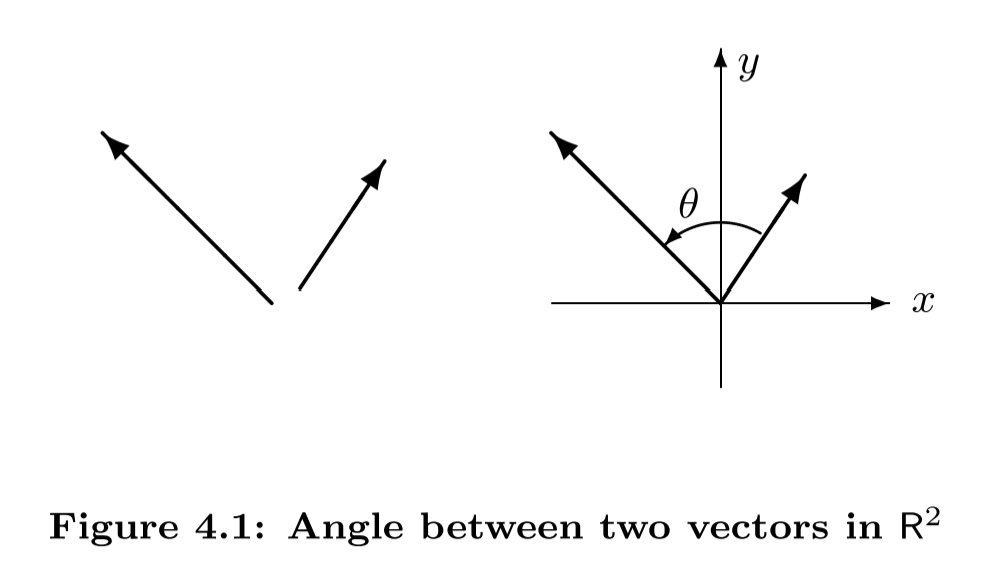
\includegraphics[width=12cm]{images/figure-4-1.png}

If \(\beta = \{ u, v \}\) is an ordered basis for \(\SET{R}^2\), we define the \textbf{orientation} of \(\beta\) to be the \emph{real number}
\[
    \mathcal{O} \begin{pmatrix} u \\ v \end{pmatrix}
    = \frac {\det\begin{pmatrix} u \\ v \end{pmatrix}} {\left| \det\begin{pmatrix} u \\ v \end{pmatrix} \right| }.
\]
(The denominator of this fraction is nonzero by \THM{4.2}.)
Clearly,
\[
    \mathcal{O} \begin{pmatrix} u \\ v \end{pmatrix} = \pm 1.
\]
\end{additional definition}

\begin{additional definition} \label{adef 4.2}
Notice that
\[
    \mathcal{O} \begin{pmatrix} e_1 \\ e_2 \end{pmatrix} = 1.
    \text{ and }
    \mathcal{O} \begin{pmatrix} e_1 \\ \RED{-e_2} \end{pmatrix} = -1.
\]
Recall that a coordinate system \(\{ u, v \}\) is called \textbf{right-handed} if \(u\) can be \emph{rotated in a counterclockwise} direction through an angle \(\theta\) \((0 < \theta < \pi\))to coincide with \(v\).
Otherwise \(\{ u, v \}\) is called a \textbf{left-handed system}.
(See Figure 4.2.)

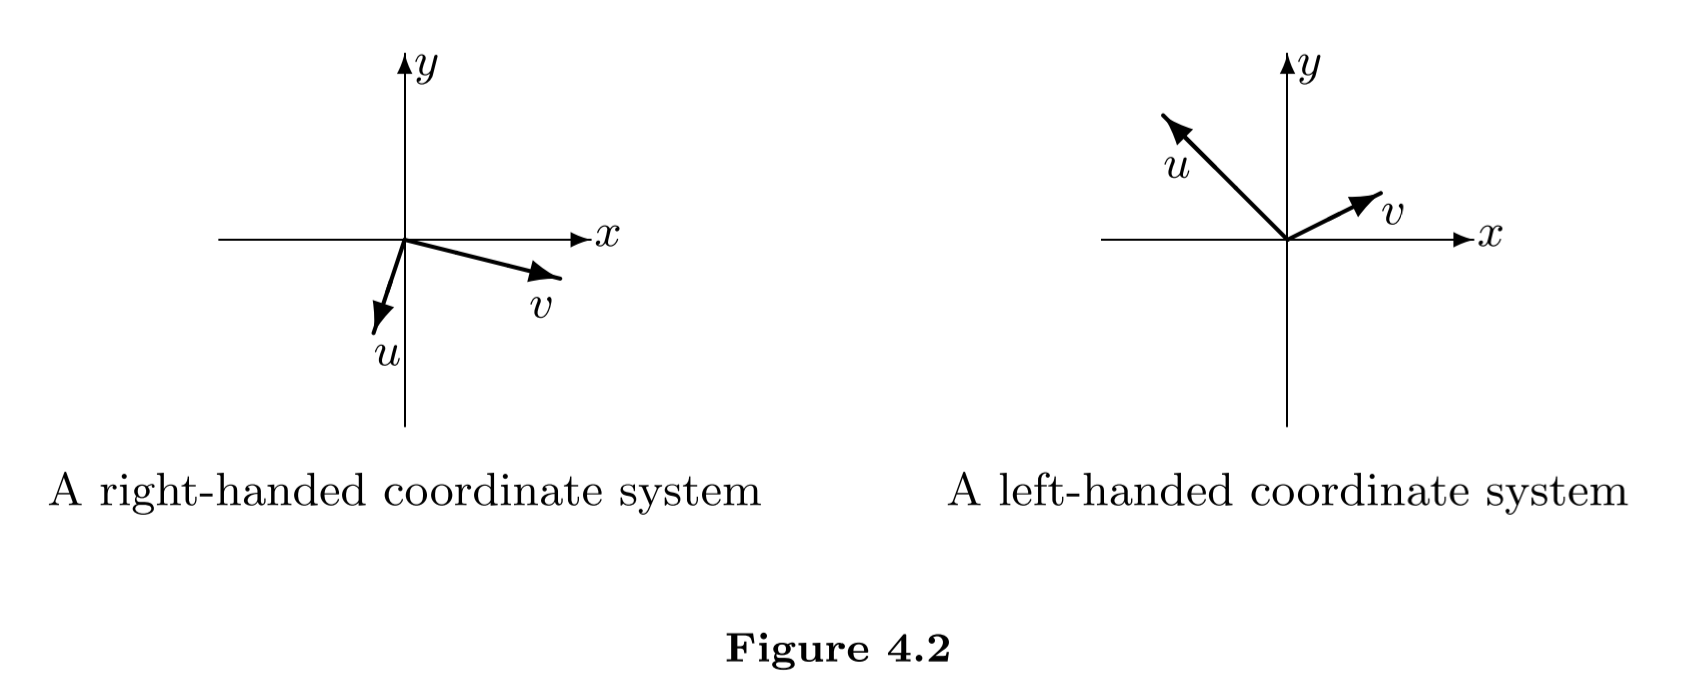
\includegraphics[width=16cm]{images/figure-4-2.png}

In general (see \EXEC{4.1.13}),
\[
    \mathcal{O} \begin{pmatrix} u \\ v \end{pmatrix} = 1.
\]
if and only if the ordered basis \(\{ u, v \}\) forms a right-banded coordinate system.
\end{additional definition}

\begin{remark} \label{remark 4.1.3}
For convenience, we also define
\[
    \mathcal{O} \begin{pmatrix} u \\ v \end{pmatrix} = 1.
\]
if \(\{ u, v \}\) is linearly \textbf{dependent}.
\end{remark}

Any ordered set \(\{ u, v \}\) in \(\SET{R}^2\) determines a parallelogram in the following manner.
Regarding \(u\) and \(v\) as arrows emanating from the origin of \(\SET{R}^2\), we call the \textbf{parallelogram} having \(u\) and \(v\) as \emph{adjacent sides} the \textbf{parallelogram
determined by \(u\) and \(v\)}.
(See Figure 4.3.)

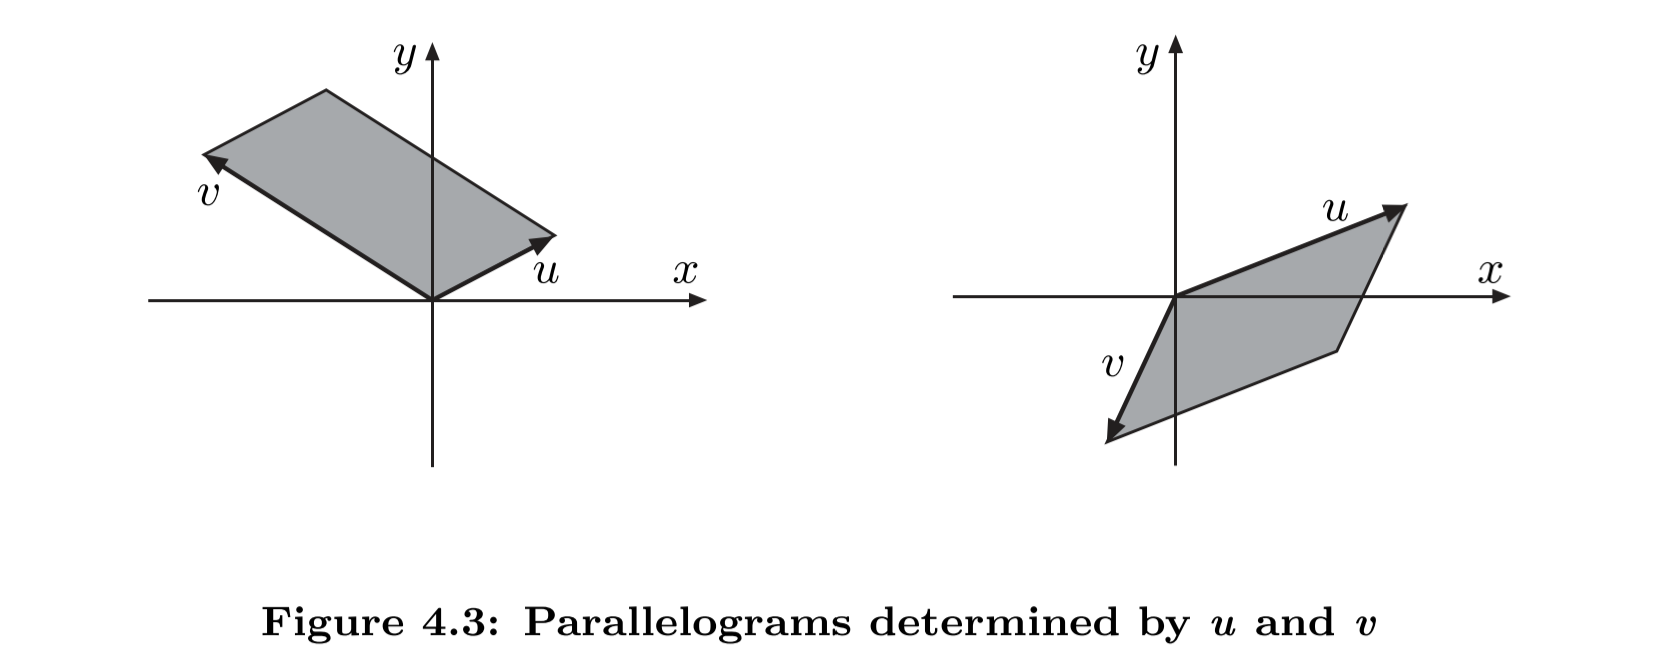
\includegraphics[width=16cm]{images/figure-4-3.png}

\begin{remark} \label{remark 4.1.4}
Observe that if the set \(\{ u, v \}\) is linearly \textbf{dependent} (i.e., if \(u\) and \(v\) are \emph{parallel}),
then the ``parallelogram'' determined by \(u\) and \(v\) is \emph{actually a line segment}, which we consider to be a
\href{https://www.wikiwand.com/en/Degeneracy_(mathematics)}{\textbf{degenerate}} parallelogram having area zero.
\end{remark}

\begin{additional theorem} \label{athm 4.1}
We have
\[
    \mathcal{A}\begin{pmatrix} u \\ v \end{pmatrix}
    = \left| \det \begin{pmatrix} u \\ v \end{pmatrix} \right|.
\]
Where \(\mathcal{A}\begin{pmatrix} u \\ v \end{pmatrix}\) denotes the area of the parallelogram determined by \(u\) and \(v\).
The proof is in the long and messy discussion below.
\end{additional theorem}

\begin{proof}
Since
\[
    \det \begin{pmatrix} u \\ v \end{pmatrix}
\]
may be negative, we cannot expect that
\[
    \mathcal{A}\begin{pmatrix} u \\ v \end{pmatrix} = \det \begin{pmatrix} u \\ v \end{pmatrix}.
\]
But \textbf{we can prove that}
\begin{equation} \label{area.formula}
    \mathcal{A}\begin{pmatrix} u \\ v \end{pmatrix} = \mathcal{O}\begin{pmatrix} u \\ v \end{pmatrix} \cdot \det \begin{pmatrix} u \\ v \end{pmatrix}
\end{equation}
from which it clearly follows that
\begin{equation} \label{simplified.area.formula}
    \mathcal{A}\begin{pmatrix} u \\ v \end{pmatrix} = \left| \det \begin{pmatrix} u \\ v \end{pmatrix} \right|.
\end{equation}
Our argument that \ref{area.formula} is correct employs a technique that, although somewhat indirect, can be \emph{generalized to \(\SET{R}^n\)}.
(Hence we will employ a similar argument in \SEC{4.2} and \SEC{4.3}.)

First, since
\[
    \mathcal{O} \begin{pmatrix} u \\ v \end{pmatrix} = \pm 1,
\]
we may multiply both sides of \ref{area.formula} by
\[
    \mathcal{O} \begin{pmatrix} u \\ v \end{pmatrix}
\]
to obtain the equivalent form
\[
    \mathcal{O}\begin{pmatrix} u \\ v \end{pmatrix} \mathcal{A}\begin{pmatrix} u \\ v \end{pmatrix} = \left(\mathcal{O}\begin{pmatrix} u \\ v \end{pmatrix}\right)^2 \cdot \det \begin{pmatrix} u \\ v \end{pmatrix} =
    1 \cdot \det \begin{pmatrix} u \\ v \end{pmatrix} =
    \det \begin{pmatrix} u \\ v \end{pmatrix},
\]
that is,
\begin{equation} \label{equivalent.area.formula}
    \det \begin{pmatrix} u \\ v \end{pmatrix}
    = \mathcal{O}\begin{pmatrix} u \\ v \end{pmatrix} \mathcal{A}\begin{pmatrix} u \\ v \end{pmatrix}.
\end{equation}
Hence \ref{equivalent.area.formula} is true if and only if \ref{area.formula} is true.
So we prove \ref{equivalent.area.formula} instead.

But first we \textbf{define} the function
\begin{equation} \label{def.delta}
    \delta \begin{pmatrix} u \\ v \end{pmatrix}
    = \mathcal{O}\begin{pmatrix} u \\ v \end{pmatrix}
      \cdot \mathcal{A}\begin{pmatrix} u \\ v \end{pmatrix}.
\end{equation}
And we will verify that \ref{def.delta} satisfies the three conditions of \EXEC{4.1.11}, and hence by \EXEC{4.1.11}, \(\delta\) is actually equal to \(\det\);
that is, \ref{equivalent.area.formula} is correct. (hence \ref{area.formula} is correct.)

\begin{note}
I recommend read \EXEC{4.1.11} first and go back to this very long and messy proof.
\end{note}

So we prove that \(\delta\) satisfies the three conditions in \EXEC{4.1.11} below:
\begin{enumerate}
\item For the first condition in \EXEC{4.1.11}, we need to show the four equations(given appropriate \(u, v, u_1, u_2, v_1, v_2, c\)):
\begin{align*}
    \delta \begin{pmatrix} u \\ cv \end{pmatrix}
    & = c \cdot \delta \begin{pmatrix} u \\ v \end{pmatrix} \\
    \delta \begin{pmatrix} cu \\ v \end{pmatrix}
    & = c \cdot \delta \begin{pmatrix} u \\ v \end{pmatrix} \\
    \delta \begin{pmatrix} u \\ v_1 + v_2 \end{pmatrix}
    & = \delta \begin{pmatrix} u \\ v_1 \end{pmatrix}
      + \delta \begin{pmatrix} u \\ v_2 \end{pmatrix} \\
    \delta \begin{pmatrix} u_1 + u_2 \\ v \end{pmatrix}
    & = \delta \begin{pmatrix} u_1 \\ v \end{pmatrix}
      + \delta \begin{pmatrix} u_2 \\ v \end{pmatrix}
\end{align*}
We begin by showing that for any real number \(c\)
\[
    \delta \begin{pmatrix} u \\ cv \end{pmatrix}
    = c \cdot \delta \begin{pmatrix} u \\ v \end{pmatrix}.
\]
Observe that this equation is valid if \(c = 0\) because
\begin{align*}
    \delta \begin{pmatrix} u \\ cv \end{pmatrix}
        & = \delta \begin{pmatrix} u \\ 0 \end{pmatrix} & \text{of course} \\
        & = \mathcal{O}\begin{pmatrix} u \\ 0 \end{pmatrix} \cdot \mathcal{A}\begin{pmatrix} u \\ v \end{pmatrix} & \text{by def in \ref{def.delta}} \\
        & = 1 \cdot \mathcal{A}\begin{pmatrix} u \\ v \end{pmatrix} & \text{by \RMK{4.1.3}} \\
        & = 1 \cdot 0 & \text{by \RMK{4.1.4}} \\
        & = 0 & \text{of course} \\
        & = 0 \cdot \delta \begin{pmatrix} u \\ v \end{pmatrix} & \text{of course} \\
        & = c \cdot \delta \begin{pmatrix} u \\ v \end{pmatrix}.
\end{align*}
So assume that \(c \ne 0\).
Regarding \(cv\) as the \emph{base of the parallelogram} determined by \(u\) and \(cv\), (by geometry formula) we see that
\begin{align*}
    \mathcal{A}\begin{pmatrix}
        u \\ cv
    \end{pmatrix}
    & = \text{(base of \(cv\) and \(u\))} \X \text{(altitude of \(cv\) and \(u\))} & \text{by geometry formula} \\
    & = \abs{c} \cdot (\text{length of } v) \X (\text{altitude of \(cv\) and \(u\)}) \\
    & = \abs{c} \cdot (\text{length of } v) \X (\text{altitude \textbf{of \(v\) and \(u\)}}) \\
    & \text{\ \ \ \ \ \ (since the altitude of these parallelograms are)} \\
    & \text{\ \ \ \ \ \ (the same; see Figure 4.4.)} \\
    & = \abs{c} \mathcal{A}\begin{pmatrix}
        u \\ v
    \end{pmatrix}. & \text{by geometry formula}
\end{align*}
So we have
\[
    \mathcal{A}\begin{pmatrix}
        u \\ cv
    \end{pmatrix}
    = \abs{c} \mathcal{A}\begin{pmatrix}
        u \\ v
    \end{pmatrix}. \text{ -- \MAROON{(a.1)}}
\]

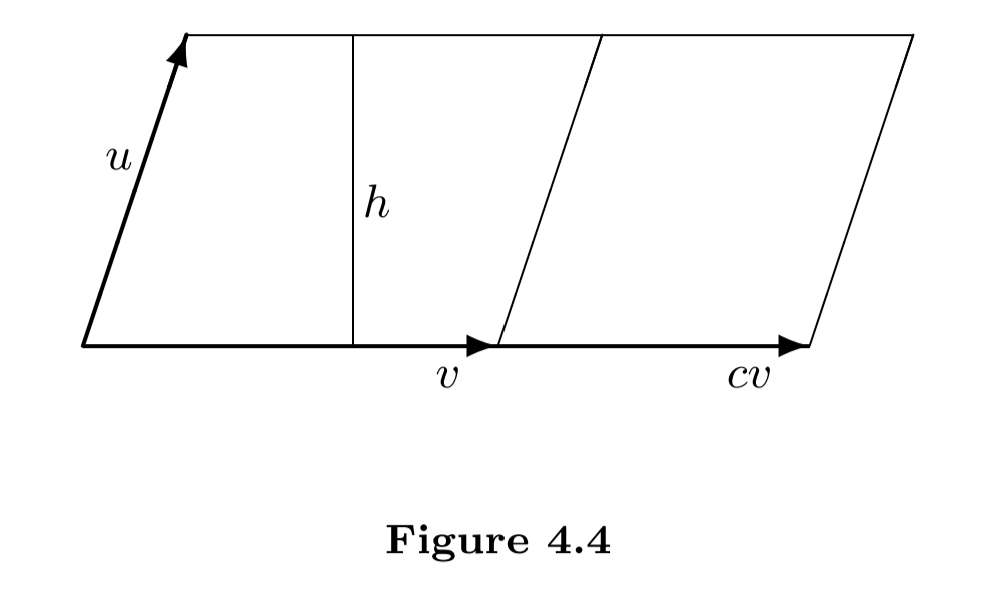
\includegraphics[width=10cm]{images/figure-4-4.png}

Hence
\begin{align*}
    \delta \begin{pmatrix}
        u \\ cv
    \end{pmatrix}
    & = \mathcal{O}\begin{pmatrix} u \\ cv \end{pmatrix} \cdot \mathcal{A}\begin{pmatrix} u \\ cv \end{pmatrix} & \text{by def in \ref{def.delta}} \\
    & = \left[\frac{c}{\abs{c}} \mathcal{O}\begin{pmatrix} u \\ v \end{pmatrix}\right] \mathcal{A}\begin{pmatrix} u \\ cv \end{pmatrix} & \text{need to prove but trivial by def of \(\mathcal{O}\)} \\
    & = \left[\frac{c}{\abs{c}} \mathcal{O}\begin{pmatrix} u \\ v \end{pmatrix}\right] \left[\abs{c} \mathcal{A}\begin{pmatrix} u \\ v \end{pmatrix}\right] & \text{by \MAROON{(a.1)}} \\
    & = c \cdot \mathcal{O}\begin{pmatrix} u \\ v \end{pmatrix} \cdot \mathcal{A}\begin{pmatrix} u \\ v \end{pmatrix} & \text{of course} \\
    & = c \cdot \delta \begin{pmatrix}
        u \\ v
    \end{pmatrix}. & \text{by def in \ref{def.delta}}
\end{align*}
A similar argument shows
\[
    \delta \begin{pmatrix}
        cu \\ v
    \end{pmatrix}
    = c \cdot \delta \begin{pmatrix}
        u \\ v
    \end{pmatrix}.
\]

So currently we have shown that
\[
    \delta \begin{pmatrix}
        u \\ cv
    \end{pmatrix}
    = c \cdot \delta \begin{pmatrix}
        u \\ v
    \end{pmatrix}.
    \text{ and }
    \delta \begin{pmatrix}
        cu \\ v
    \end{pmatrix}
    = c \cdot \delta \begin{pmatrix}
        u \\ v
    \end{pmatrix}. \text{ -- \BLUE{(1)}}
\]

Now before we prove the remaining two equations, we first prove that
\[
    \delta \begin{pmatrix}
        u \\ a\RED{u} + bw
    \end{pmatrix}
    = b \cdot \delta \begin{pmatrix}
        u \\ w
    \end{pmatrix}
\]
for any \(u, w \in \SET{R}^2\).
Because the parallelograms determined by \(u\) and \(w\) and by \(u\) and \(u + w\) \emph{have a common base} \(u\) and the same altitude (see Figure 4.5), (by geometry) it follows that
\[
    \mathcal{A} \begin{pmatrix}
        u \\ w
    \end{pmatrix}
    = \mathcal{A} \begin{pmatrix}
        u \\ \RED{u} + w
    \end{pmatrix}
\]
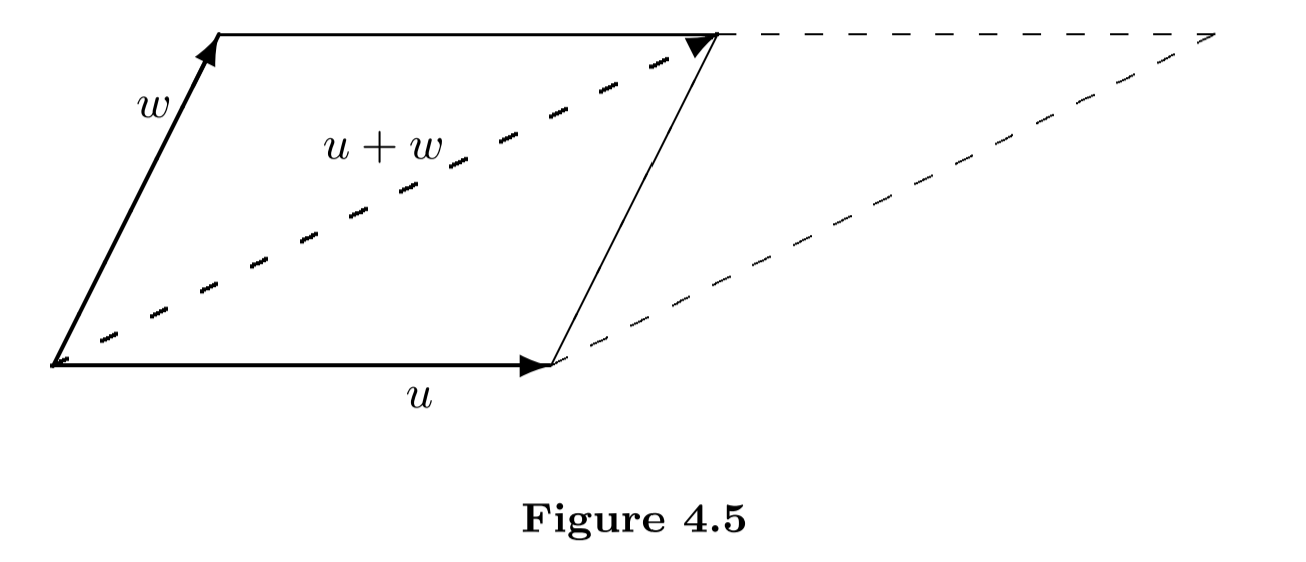
\includegraphics[width=14cm]{images/figure-4-5.png}

If \(a = 0\), then
\begin{align*}
    \delta \begin{pmatrix} u \\ au + bw \end{pmatrix}
    = \delta \begin{pmatrix} u \\ 0 + bw \end{pmatrix}
    & = \delta \begin{pmatrix} u \\ bw \end{pmatrix} \\
    & = b \cdot \delta \begin{pmatrix} u \\ w \end{pmatrix}. & \text{by \BLUE{(1)}}
\end{align*}
Otherwise, if \(a \ne 0\), then
\begin{align*}
    \delta \begin{pmatrix}
        u \\ au + bw
    \end{pmatrix}
    & = \delta \begin{pmatrix}
        u \\ a(u + \frac{b}{a}w)
    \end{pmatrix} & \text{of course} \\
    & = a \cdot \delta \begin{pmatrix}
        u \\ u + \frac{b}{a}w
    \end{pmatrix} & \text{by \BLUE{(1)}} \\
    & = a \cdot \delta \begin{pmatrix}
        u \\ \frac{b}{a}w
    \end{pmatrix} & \text{(indirectly) by Figure 4.5} \\
    & = a \left( \frac{b}{a} \right) \cdot \delta \begin{pmatrix}
        u \\ w
    \end{pmatrix} & \text{by \BLUE{(1)} again} \\
    & = b \cdot \delta \begin{pmatrix}
        u \\ w
    \end{pmatrix} & \text{of course}.
\end{align*}
So in all cases, we have
\[
    \delta \begin{pmatrix}
        u \\ au + bw
    \end{pmatrix}
    = b \cdot \delta \begin{pmatrix}
        u \\ w
    \end{pmatrix}. \text{ -- \BLUE{(2)}}
\]
Finally, we now are able to show that
\[
    \delta \begin{pmatrix}
        u \\ v_1 + v_2
    \end{pmatrix}
    = \delta \begin{pmatrix}
        u \\ v_1
    \end{pmatrix}
    + \delta \begin{pmatrix}
        u \\ v_2
    \end{pmatrix}
\]
for all \(u, v_1, v_2 \in \SET{R}^2\).
Since the result is immediate if \(u = 0\)
(that will cause every term to be zero, since the area of the corresponding parallelogram will we zero),
we assume that \(u \ne 0\).
Choose any vector \(w \in \SET{R}^2\) such that \(\{ u, w \}\) is \emph{\LID{}}.
Then for any vectors \(v_1, v_2 \in \SET{R}^2\) there exist (unique) scalars \(a_i\) and \(b_i\) such that
\[
    v_i = a_i u + b_i w \ \  (i = 1, 2). \text{ -- \MAROON{(a.2)}}
\]
Thus
\begin{align*}
    \delta \begin{pmatrix}
        u \\ v_1 + v_2
    \end{pmatrix}
    & = \delta \begin{pmatrix}
            u \\ (a_1 + a_2) \RED{u} + (b_1 + b_2) w
        \end{pmatrix} & \text{by \MAROON{(a.2)}} \\
    & = (b_1 + b_2) \delta \begin{pmatrix}
            u \\ w
        \end{pmatrix} & \text{by \BLUE{(2)}} \\
    & = b_1 \delta \begin{pmatrix}
            u \\ w
        \end{pmatrix}
      + b_2 \delta \begin{pmatrix}
            u \\ w
        \end{pmatrix} & \text{of course} \\
    & = \delta \begin{pmatrix}
            u \\ a_1 u + b_1 w
        \end{pmatrix}
      + \delta \begin{pmatrix}
            u \\ a_2 u + b_2 w
        \end{pmatrix} & \text{again by \BLUE{(2)}} \\
    & = \delta \begin{pmatrix}
            u \\ v_1
        \end{pmatrix}
      + \delta \begin{pmatrix}
            u \\ v_2
        \end{pmatrix} & \text{by \MAROON{(a.2)}}
\end{align*}
A similar argument shows that
\[
    \delta \begin{pmatrix}
        u_1 + u_2 \\ v
    \end{pmatrix}
    = \delta \begin{pmatrix}
            u_1 \\ v
        \end{pmatrix}
      + \delta \begin{pmatrix}
            u_2 \\ v
        \end{pmatrix}
\]
for all \(u_1, u_2, v \in \SET{R}^2\).

So finally, we have proved that the four equations in the first condition of \EXEC{4.1.11} are satisfied by definition of \(\delta\) in \ref{def.delta}.

\item
Since (by geometry) \(\mathcal{A} \begin{pmatrix} u \\ u \end{pmatrix} = 0\), it follows that
\begin{align*}
    \delta \begin{pmatrix} u \\ u \end{pmatrix}
    & = \mathcal{O} \begin{pmatrix} u \\ u \end{pmatrix} \cdot \mathcal{A} \begin{pmatrix} u \\ u \end{pmatrix} & \text{by def in \ref{def.delta}} \\
    & = 0
\end{align*}
for any \(u \in \SET{R}^2\).

\item
Because (by geometry) the parallelogram determined by \(e_1\) and \(e_2\) is the \emph{unit square},
\begin{align*}
    \delta(I_2)
    & = \delta \begin{pmatrix} e_1 \\ e_2 \end{pmatrix} \\
    & = \mathcal{O} \begin{pmatrix} e_1 \\ e_2 \end{pmatrix} \cdot \mathcal{A} \begin{pmatrix} e_1 \\ e_2 \end{pmatrix} & \text{by def in \ref{def.delta}} \\
    & = 1 \cdot \mathcal{A} \begin{pmatrix} e_1 \\ e_2 \end{pmatrix} & \text{of course (by calculation)} \\
    & = 1 \cdot 1 & \text{since the parallelogram is the unit square} \\
    & = 1.
\end{align*}
\end{enumerate}

Therefore, \(\delta\) defined in \ref{def.delta} satisfies the three conditions of \EXEC{4.1.11}, and hence \(\delta = \det\).
Hence \ref{equivalent.area.formula}, \ref{area.formula} and \ref{simplified.area.formula} are correct;
that is,
\[
    \mathcal{A}\begin{pmatrix} u \\ v \end{pmatrix}
    = \mathcal{O}\begin{pmatrix} u \\ v \end{pmatrix} \cdot \det \begin{pmatrix} u \\ v \end{pmatrix}
    = \left| \det \begin{pmatrix} u \\ v \end{pmatrix} \right|.
\]
\end{proof}

Thus we see, for example, that the area of the parallelogram determined by \(u = (-1, 5)\) and \(v = (4, -2)\) is
\[
    \left| \det \begin{pmatrix}
        u \\ v
    \end{pmatrix} \right|
    = \left| \det \begin{pmatrix}
        -1 & 5 \\ 4 & -2
    \end{pmatrix} \right|
    = 18.
\]

\exercisesection

\begin{exercise} \label{exercise 4.1.1}
Label the following statements as true or false.
\begin{enumerate}
\item The function \(\det : M_{2 \X 2}(F) \to F\) is a linear transformation.
\item The determinant of a \(2 \X 2\) matrix is a linear function of each row of the matrix when the other row is held fixed.
\item If \(A \in M_{2 \X 2}(F)\) and \(\det(A) = 0\), then \(A\) is invertible.
\item If \(u\) and \(v\) are vectors in \(\SET{R}^2\) emanating from the origin, then the area of the parallelogram having \(u\) and \(v\) as adjacent sides is
\[
    \det \begin{pmatrix} u \\ v \end{pmatrix}.
\]
\item A coordinate system is \emph{right-handed} if and only if its orientation equals \(1\).
\end{enumerate}
\end{exercise}

\begin{proof} \ 

\begin{enumerate}
\item False by \RMK{4.1.1}.
\item True by \THM{4.1}.
\item False, by \THM{4.2}, \(A\) is \emph{not} invertible.
\item False, by \ATHM{4.1}, the areas is
\[
    \left| \det \begin{pmatrix} u \\ v \end{pmatrix} \right|.
\]
\item True by \EXEC{4.1.13}.
\end{enumerate}
\end{proof}

\begin{exercise} \label{exercise 4.1.2}
Compute the determinants of the following matrices in  \(M_{2 \X 2}(\SET{R})\).

(a) \(\left(\begin{array}{rr} 6 & -3 \\ 2 & 4 \end{array}\right)\)
(b) \(\left(\begin{array}{rr} -5 & 2 \\ 6 & 1 \end{array}\right)\)
(c) \(\left(\begin{array}{rr} 8 & 0 \\ 3 & -1 \end{array}\right)\)
\end{exercise}

\begin{proof} \ 

\begin{enumerate}
\item
\[
    \det \left(\begin{array}{rr} 6 & -3 \\ 2 & 4 \end{array}\right) = 6 \cdot 4 - (-3) \cdot 2 = 30.
\]
\item
\[
    \det \left(\begin{array}{rr} -5 & 2 \\ 6 & 1 \end{array}\right) = -5 \cdot 1 - 2 \cdot 6 = -17.
\]
\item
\[
    \det \left(\begin{array}{rr} 8 & 0 \\ 3 & -1 \end{array}\right) = 8 \cdot (-1) - 0 \cdot 3 = -8.
\]
\end{enumerate}
\end{proof}

\begin{exercise} \label{exercise 4.1.3}
Compute the determinants of the following matrices in  \(M_{2 \X 2}(\SET{C})\).

(a) \(\left(\begin{array}{rr} -1 + \iu & 1 - 4\iu \\ 3 + 2\iu & 2 - 3\iu \end{array}\right)\)
(b) \(\left(\begin{array}{rc} 5 - 2\iu & 6 + 4\iu \\ -3 + \iu & 7\iu \end{array}\right)\)
(c) \(\left(\begin{array}{rr} 2\iu & 3 \\ 4 & 6\iu \end{array}\right)\)
\end{exercise}

\begin{proof} \ 

\begin{enumerate}
\item
\[
    \det \left(\begin{array}{rr} -1 + \iu & 1 - 4\iu \\ 3 + 2\iu & 2 - 3\iu \end{array}\right)
    = (-1 + \iu) \cdot (2 - 3\iu) - (1 - 4\iu) \cdot (3 + 2\iu)
    = -10 + 15\iu.
\]
\item
\[
    \det \left(\begin{array}{rc} 5 - 2\iu & 6 + 4\iu \\ -3 + \iu & 7\iu \end{array}\right)
    = (5 - 2\iu) \cdot (7\iu) - (6 + 4\iu) \cdot (-3 + \iu)
    = -8 + 29\iu.
\]
\item
\[
    \det \left(\begin{array}{rr} 2\iu & 3 \\ 4 & 6\iu \end{array}\right)
    = 2\iu \cdot 6\iu - 3 \cdot 4
    = -24.
\]
\end{enumerate}
\end{proof}

\begin{exercise} \label{exercise 4.1.4}
For each of the following pairs of vectors \(u\) and \(v\) in \(\SET{R}^2\), compute the area of the parallelogram determined by \(u\) and \(v\).
\begin{enumerate}
\item \(u = (3, -2)\) and \(v = (2, 5)\).
\item \(u = (1, 3)\) and \(v = (-3, 1)\).
\item \(u = (4, -1)\) and \(v = (-6, -2)\).
\item \(u = (3, 4)\) and \(v = (2, -6)\).
\end{enumerate}
\end{exercise}

\begin{proof} \ 

\begin{enumerate}
\item
\[
    \left| \det \begin{pmatrix} 3 & -2 \\ 2 & 5
\end{pmatrix} \right| = |3 \cdot 5 - (-2) \cdot 2| = 19.
\]

\item
\[
    \left| \det \begin{pmatrix} 1 & 3 \\ -3 & 1
\end{pmatrix} \right| = |1 \cdot 1 - 3 \cdot (-3)| = 10.
\]

\item
\[
    \left| \det \begin{pmatrix} 4 & -1 \\ -6 & -2
\end{pmatrix} \right| = |4 \cdot (-2) - (-1) \cdot (-6)| = 14.
\]

\item
\[
    \left| \det \begin{pmatrix} 3 & 4 \\ 2 & -6
\end{pmatrix} \right| = |3 \cdot (-6) - 4 \cdot 2| = 26.
\]
\end{enumerate}
\end{proof}

\begin{exercise} \label{exercise 4.1.5}
Prove that if \(B\) is the matrix obtained by \emph{interchanging} the rows of a \(2 \X 2\) matrix \(A\), then \(\det(B) = -\det(A)\).
\end{exercise}

\begin{proof}
Let
\[
    A = \begin{pmatrix} A_{11} & A_{12} \\ A_{21} & A_{22} \end{pmatrix}
    \text{, then }
    B = \begin{pmatrix} A_{21} & A_{22} \\ A_{11} & A_{12} \end{pmatrix}.
\]
So by \DEF{4.1}, \(\det(A) = A_{11} A_{22} - A_{12} A_{21}\), and \(\det(B) = A_{21} A_{12} - A_{22} A_{11} = A_{12} A_{21} - A_{11} A_{22} = -(A_{11} A_{22} - A_{12} A_{21}) = -\det(A)\), as desired.
\end{proof}

\begin{exercise} \label{exercise 4.1.6}
Prove that if the two \emph{columns} of \(A \in M_{2 \X 2}(F)\) are identical, then \(\det(A) = 0\).
\end{exercise}

\begin{proof}
If columns of \(A\) are identical, then (by \CH{3}) \(A\) is not invertible, and by \THM{4.2}, \(\det(A) = 0\).
\end{proof}

\begin{exercise} \label{exercise 4.1.7}
Prove that \(\det(A^\top) = \det(A)\) for any \(A \in M_{2 \X 2}(F)\).
\end{exercise}

\begin{proof}
Let
\[
    A = \begin{pmatrix} A_{11} & A_{12} \\ A_{21} & A_{22} \end{pmatrix}
\]
then
\[
    A^\top = \begin{pmatrix} A_{11} & A_{21} \\ A_{12} & A_{22} \end{pmatrix}
\]
So by \DEF{4.1}, \(\det(A) = A_{11} A_{22} - A_{12} A_{21}\), and \(\det(A^\top) = A_{11} A_{22} - A_{21} A_{12} = A_{11} A_{22} - A_{12} A_{21} = \det(A)\), as desired.
\end{proof}

\begin{exercise} \label{exercise 4.1.8}
Prove that if \(A \in M_{2 \X 2}(F)\) is \emph{upper triangular}, then \(\det(A)\) equals the \emph{product of the diagonal} entries of \(A\).
\end{exercise}

\begin{proof}
Since \(A\) is upper triangular, \(A\) has the form
\[
    A^\top = \begin{pmatrix} A_{11} & A_{12} \\ \RED{0} & A_{22} \end{pmatrix}
\]
And by \DEF{4.1}, \(\det(A) = A_{11} A_{22} - A_{12} \cdot 0 = A_{11} A_{22}\), which is the product of the diagonal entries of \(A\).
\end{proof}

\begin{exercise} \label{exercise 4.1.9}
Prove that \(\det(AB) = \det(A) \cdot \det(B)\) for any \(A, B \in M_{2 \X 2}(F)\).
\end{exercise}

\begin{proof}
Let
\[
    A = \begin{pmatrix} a_1 & a_2 \\ a_3 & a_4 \end{pmatrix},
    B = \begin{pmatrix} b_1 & b_2 \\ b_3 & b_4 \end{pmatrix}.
\]
Then (by calculation)
\[
    AB = \begin{pmatrix}
        a_1 b_1 + a_2 b_3 & a_1 b_2 + a_2 b_4 \\
        a_3 b_1 + a_4 b_3 & a_3 b_2 + a_4 b_4
    \end{pmatrix}.
\]
So by \DEF{4.1},
\begin{align*}
    \det(A) & = a_1 a_4 - a_2 a_3, \\
    \det(B) & = b_1 b_4 - b_2 b_3, \\
    \det(A)\det(B) & = (a_1 a_4 - a_2 a_3)(b_1 b_4 - b_2 b_3) \\
                   & = (a_1 a_4 b_1 b_4 - a_1 a_4 b_2 b_3 - a_2 a_3 b_1 b_4 + a_2 a_3 b_2 b_3) \text{ -- \MAROON{(1)}}, \\
    \det(AB) & = (a_1 b_1 + a_2 b_3)(a_3 b_2 + a_4 b_4) - (a_1 b_2 + a_2 b_4)(a_3 b_1 + a_4 b_3) \\
             & = (\GREEN{a_1 b_1 a_3 b_2} + a_1 b_1 a_4 b_4 + a_2 b_3 a_3 b_2 + \BLUE{a_2 b_3 a_4 b_4}) \\
             & \ \ \ \  \RED{-} (\GREEN{a_1 b_2 a_3 b_1} + a_1 b_2 a_4 b_3 + a_2 b_4 a_3 b_1 + \BLUE{a_2 b_4 a_4 b_3}) \\
             & = (a_1 b_1 a_4 b_4 + a_2 b_3 a_3 b_2) - (a_1 b_2 a_4 b_3 + a_2 b_4 a_3 b_1) \\
             & = (a_1 a_4 b_1 b_4 + a_2 a_3 b_2 b_3) - (a_1 a_4 b_2 b_3 + a_2 a_3 b_1 b_4) \\
             & = \MAROON{(1)} = \det(A)\det(B),
\end{align*}
as desired.
\end{proof}

\begin{exercise} \label{exercise 4.1.10}
The \textbf{classical adjoint} of a \(2 \X 2\) matrix \(A \in M_{2 \X 2}(F)\) is the matrix
\[
    C = \begin{pmatrix} A_{22} & -A_{12} \\ -A_{21} & A_{11} \end{pmatrix}.
\]
Prove that
\begin{enumerate}
\item \(CA = AC = [\det(A)]I\).
\item \(\det(C) = \det(A)\).
\item The classical adjoint of \(A^\top\) is \(C^\top\).
\item If \(A\) is invertible, then \(A^{-1} = [\det(A)]^{-1}C\).
\end{enumerate}
\end{exercise}

\begin{proof} \ 

\begin{enumerate}
\item
\begin{align*}
    AC & =
        \begin{pmatrix}
            A_{11} & A_{12} \\
            A_{21} & A_{22}
        \end{pmatrix}
        \begin{pmatrix}
            A_{22} & -A_{12} \\
            -A_{21} & A_{11}
        \end{pmatrix} \\
      & = \begin{pmatrix}
            A_{11} A_{22} - A_{12} A_{21} & -A_{11} A_{12} + A_{12} A_{11} \\
            A_{21} A_{22} - A_{22} A_{21} & - A_{21} A_{12} + A_{22} A_{11}
        \end{pmatrix}
      & = \begin{pmatrix}
          \det(A) & 0 \\
          0 & \det(A)
      \end{pmatrix}
      & = \det(A) \cdot I_2.
\end{align*}
and
\begin{align*}
   CA & =
        \begin{pmatrix}
            A_{22} & -A_{12} \\
            -A_{21} & A_{11}
        \end{pmatrix}
        \begin{pmatrix}
            A_{11} & A_{12} \\
            A_{21} & A_{22}
        \end{pmatrix} \\
      & = \begin{pmatrix}
            A_{22} A_{11} - A_{12} A_{21} & A_{22} A_{12} - A_{12} A_{22} \\
            -A_{21} A_{11} + A_{11} A_{21} & - A_{21} A_{12} + A_{11} A_{22}
        \end{pmatrix}
      & = \begin{pmatrix}
          \det(A) & 0 \\
          0 & \det(A)
      \end{pmatrix}
      & = \det(A) \cdot I_2. 
\end{align*}

\item
We have
\[
    \det(C) = A_{22}A_{11} - (-A_{12})(-A_{21}) = A_{22} A_{11} - A_{12} A_{21} = \det(A).
\]

\item First,
\[
    A^\top = \begin{pmatrix}
        A_{11} & A_{21} \\
        A_{12} & A_{22}
    \end{pmatrix}
\]
so by def, the adjoint matrix of \(A^\top\) is
\[
    \begin{pmatrix}
        A_{22}^\top & -A_{12}^\top \\
        -A_{21}^\top & A_{11}^\top    
    \end{pmatrix}
\]
which by definition of transpose (of each entry) is
\[
    \begin{pmatrix}
        A_{22} & -A_{21} \\
        -A_{12} & A_{11}
    \end{pmatrix}
\]
which by definition of transpose again is \(C^\top\).

\item
We have
\begin{align*}
    A ([\det(A)]^{-1} C)
    & = [\det(A)]^{-1} (AC) & \text{of course, or by \THM{2.12}(b)} \\
    & = [\det(A)]^{-1} [\det(A)] I & \text{by part(a)} \\
    & = I.
\end{align*}
And by \ATHM{2.38}, ``one-sided'' inverse is a ``two-sided'' inverse, we have \(A^{-1} = [\det(A)]^{-1} C\).
\end{enumerate}
\end{proof}

\begin{exercise} \label{exercise 4.1.11}
Let \(\delta: M_{2 \X 2}(F) \to F\) be a function with the following three properties.
\begin{enumerate}
\item[(i)] \(\delta\) is a linear function of each row of the matrix when the other row is held fixed.
\item[(ii)] If the two rows of \(A \in M_{2 \X 2}(F)\) are identical, then \(\delta(A) = 0\).
\item[(iii)] If \(I\) is the \(2 \X 2\) identity matrix, then \(\delta(I) = 1\).
\end{enumerate}

Then
\begin{enumerate}
\item Prove that \(\delta(E) = \det(E)\) for all \textbf{elementary} matrices \(E \in M_{2 \X 2}(F)\).
\item Prove that \(\delta(EA) = \delta(E)\delta(A)\) for all \(A \in M_{2 \X 2}(F)\) and all \textbf{elementary} matrices \(E \in M_{2 \X 2}(F)\).
\end{enumerate}
\end{exercise}

\begin{proof} \ 

\begin{enumerate}
\item
We prove by cases of each type of elementary matrix.
For type 1, there are only one matrix:
\[
    E_1 = \begin{pmatrix}
        0 & 1 \\
        1 & 0
    \end{pmatrix}.
\]
It's clear that \(\det(E_1) = -1\).
Now by definition(ii) of \(\delta\), we have
\[
    \delta \begin{pmatrix} 1 & 0 \\ 1 & 0 \end{pmatrix}
    = \delta \begin{pmatrix} 0 & 1 \\ 0 & 1 \end{pmatrix}
    = \delta \begin{pmatrix} 1 & 1 \\ 1 & 1 \end{pmatrix}
    = 0 \text{ -- \MAROON{(1)}}
\]
Since each matrix above has identical rows respectively.
Then
\begin{align*}
    0 & = \delta \begin{pmatrix} 1 & 1 \\ 1 & 1 \end{pmatrix} & \text{by \MAROON{(1)}} \\
      & = \delta \begin{pmatrix} 1 & 0 \\ 1 & 1 \end{pmatrix}
          + \delta \begin{pmatrix} 0 & 1 \\ 1 & 1 \end{pmatrix} & \text{by def (i) of \(\delta\), fix row \(2\)} \\
      & = \left( \delta \begin{pmatrix} 1 & 0 \\ 1 & 0 \end{pmatrix} + \delta \begin{pmatrix} 1 & 0 \\ 0 & 1 \end{pmatrix} \right)
          + \delta \begin{pmatrix} 0 & 1 \\ 1 & 1 \end{pmatrix} & \text{by def (i) of \(\delta\), fix row \(1\)} \\
      & = (0 + 1) + \delta \begin{pmatrix} 0 & 1 \\ 1 & 1 \end{pmatrix} & \text{by \MAROON{(1)} and by def (iii) of \(\delta\)} \\
      & = 1 + \delta \begin{pmatrix} 0 & 1 \\ 1 & 1 \end{pmatrix} & \text{of course} \\
      & = 1 + \left( \delta \begin{pmatrix} 0 & 1 \\ 0 & 1 \end{pmatrix} + \delta \begin{pmatrix} 0 & 1 \\ 1 & 0 \end{pmatrix} \right) & \text{by def (i) of \(\delta\), fix row \(1\)} \\
      & = 1 + \left( 0 + \delta \begin{pmatrix} 0 & 1 \\ 1 & 0 \end{pmatrix} \right) & \text{by \MAROON{(1)}} \\
      & = 1 + \delta \begin{pmatrix} 0 & 1 \\ 1 & 0 \end{pmatrix} \\
      & = 1 + \delta(E_1)
\end{align*}
which implies \(\delta(E_1) = -1\) \MAROON{(a.1)}, which is equal to \(\det(E_1)\).

Now if \(E_2\) is a type 2 elementary matrix, we can represent \(E_2\) as
\[
    E_2 = \begin{pmatrix} c & 0 \\ 0 & 1
    \end{pmatrix}
    \text{ or }
    E_2 = \begin{pmatrix} 1 & 0 \\ 0 & c
    \end{pmatrix}
\]
We show the case of the first form; the second form is similar.
It's clear that \(\det(E_2) = c\).
And
\begin{align*}
    \delta(E_2) & = \delta \begin{pmatrix} c & 0 \\ 0 & 1 \end{pmatrix} \\
                & = c \delta \begin{pmatrix} 1 & 0 \\ 0 & 1 \end{pmatrix} & \text{by def (i) of \(\delta\), fix row \(2\)} \\
                & = c 1 & \text{by def (iii) of \(\delta\)} \\
                & = c = \det(E_2).
\end{align*}

Finally, if \(E_3\) is a type 3 elementary matrix, we can represent \(E_3\) as
\[
    E_2 = \begin{pmatrix} 1 & 0 \\ c & 1
    \end{pmatrix}
    \text{ or }
    E_2 = \begin{pmatrix} 1 & c \\ 0 & 1
    \end{pmatrix}
\]
We show the case of the first form; the second form is similar.
It's clear that \(\det(E_3) = 1\).
And
\begin{align*}
    \delta(E_3) & = \delta \begin{pmatrix} 1 & 0 \\ c & 1 \end{pmatrix} \\
                & = \delta \begin{pmatrix} 1 & 0 \\ c & 0 \end{pmatrix} + \delta \begin{pmatrix} 1 & 0 \\ 0 & 1 \end{pmatrix} & \text{by def (i) of \(\delta\), fix row \(1\)} \\
                & = c \delta \begin{pmatrix} 1 & 0 \\ 1 & 0 \end{pmatrix} + \delta \begin{pmatrix} 1 & 0 \\ 0 & 1 \end{pmatrix} & \text{by def (i) of \(\delta\), fix row \(1\)} \\
                & = c \cdot 0 + \delta \begin{pmatrix} 1 & 0 \\ 0 & 1 \end{pmatrix} & \text{by def (ii) of \(\delta\)} \\
                & = \delta \begin{pmatrix} 1 & 0 \\ 0 & 1 \end{pmatrix} & \text{of course} \\
                & = 1 & \text{by def (iii) of \(\delta\)} \\
                & = \det(E_3).
\end{align*}
So we have shown that \(\det(E) = \delta(E)\) for any \emph{elementary} matrix \(E\).

\item
Let arbitrary \(2 \X 2\) matrix
\[
    A = \begin{pmatrix}
        a_1 & a_2 \\ a_3 & a_4
    \end{pmatrix}.
\]
Then
\begin{align*}
    \delta(A) & = \delta \begin{pmatrix} a_1 & a_2 \\ a_3 & a_4 \end{pmatrix} \\
              & = \delta \begin{pmatrix} a_1 & a_2 \\ a_3 & 0 \end{pmatrix}
                + \delta \begin{pmatrix} a_1 & a_2 \\ 0 & a_4 \end{pmatrix} & \text{by (i), fix row \(1\)} \\
              & = \left(
                    \delta \begin{pmatrix} a_1 & 0 \\ a_3 & 0 \end{pmatrix}
                    + \delta \begin{pmatrix} 0 & a_2 \\ a_3 & 0 \end{pmatrix}
                \right)
                + \left(
                    \delta \begin{pmatrix} a_1 & 0 \\ 0 & a_4 \end{pmatrix}
                    + \delta \begin{pmatrix} 0 & a_2 \\ 0 & a_4 \end{pmatrix}
                \right) & \text{by (i), fix row \(1\)} \\
              & = a_1 a_3 \delta \begin{pmatrix} 1 & 0 \\ 1 & 0 \end{pmatrix}
                + a_2 a_3 \delta \begin{pmatrix} 0 & 1 \\ 1 & 0 \end{pmatrix}
                + a_1 a_4 \delta \begin{pmatrix} 1 & 0 \\ 0 & 1 \end{pmatrix}
                + a_2 a_4 \delta \begin{pmatrix} 0 & 1 \\ 0 & 1 \end{pmatrix} \\
              & \text{\ \ \ \ \  (by applying (i) multiple times)} \\
              & = a_1 a_3 \cdot 0
                + a_2 a_3 \delta \begin{pmatrix} 0 & 1 \\ 1 & 0 \end{pmatrix}
                + a_1 a_4 \delta \begin{pmatrix} 1 & 0 \\ 0 & 1 \end{pmatrix}
                + a_2 a_4 \cdot 0 & \text{by (ii)} \\
              & = a_2 a_3 \cdot (-1) + a_1 a_4 \cdot 1 & \text{by \MAROON{(a.1)} and (iii)} \\
              & = a_1 a_4 - a_2 a_3 \\
              & = \det(A).
\end{align*}
So we have \(\delta(A) = \det(A)\) \MAROON{(b.1)}.
And by \EXEC{4.1.9} we have \(\det(EA) = \det(E)\det(A)\).
But
\begin{align*}
    \det(E)\det(A) & = \delta(E)\det(A) & \text{by part(a)} \\
                   & = \delta(E)\delta(A) &  \text{by \MAROON{(b.1)}}
\end{align*}
So we have \(\det(EA) = \delta(E)\delta(A)\).
And by \MAROON{(b.1)} again we have \(\det(EA) = \delta(EA)\), so all in all, we have \(\delta(EA) = \delta(E)\delta(A)\), as desired.
\end{enumerate}
\end{proof}

\begin{exercise} \label{exercise 4.1.12}
Let \(\delta: M_{2 \X 2}(F) \to F\) be a function with properties (i), (ii), and (iii) in \EXEC{4.1.11}.
Use that exercise to prove that \(\delta(A) = \det(A)\) \textbf{for all} \(A \in M_{2 \X 2}(F)\).
(That is, \(\delta = \det\).)
(This result is generalized in \SEC{4.5}.)
\end{exercise}

\begin{proof}
This has been shown in the \MAROON{(b.1)} of \EXEC{4.1.11}.
\end{proof}

\begin{exercise} \label{exercise 4.1.13}
Let \(\{ u, v \}\) be an ordered basis for \(\SET{R}^2\).
Prove that
\[
    \mathcal{O} \begin{pmatrix} u \\ v \end{pmatrix} = 1
\]
if and only if \(\{ u, v \}\) forms a \emph{right-handed} coordinate system.
Hint: Recall the \emph{definition of a rotation} given in \EXAMPLE{2.1.2}.
\end{exercise}

\begin{proof}
Since by \ADEF{4.1},
\[
    \mathcal{O} \begin{pmatrix} u \\ v \end{pmatrix}
    = \frac
        {\det \begin{pmatrix}
            u \\ v
        \end{pmatrix}}
        {\left| \det \begin{pmatrix}
            u \\ v
        \end{pmatrix} \right|},
\]
clearly we have
\begin{center}
    \(\mathcal{O} \begin{pmatrix} u \\ v \end{pmatrix} = 1\) if and only if \(\det \begin{pmatrix} u \\ v \end{pmatrix} > 0\) -- \MAROON{(1)}.
\end{center}

On the other hand, (by the recall in \ADEF{4.2}) \( \{u, w \}\) forms a right-handed coordinate system if and only if \(u\) can be rotated by an angle \(\theta\) in a counterclockwise direction to coincide with \(w\).

Now, let's recall the definition of the rotation given in the \EXAMPLE{2.1.2}.
If \(u = (a_1, a_2)\), and \(w\) is obtained by \emph{rotating} \(u\) by an angle \(0 < \theta < \pi\) in a counterclockwise direction,
then the vector \(w\) has coordinates \(w = (a_1 \cos \theta -  a_2 \sin \theta, a_1 \sin \theta + a_2 \cos \theta )\) \MAROON{(2)}.
So we have
\begin{align*}
    \det \begin{pmatrix} u \\ w \end{pmatrix}
        & = \det
            \begin{pmatrix}
                a_1 & a_2 \\
                a_1 \cos \theta - a_2 \sin \theta & a_1 \sin \theta + a_2 \cos \theta
            \end{pmatrix} & \text{by \MAROON{(2)}} \\
        & = a_1(a_1 \sin \theta + a_2 \cos \theta) - a_2(a_1 \cos \theta - a_2 \sin \theta) \\
        & = a_1^2 \sin \theta + a_1 a_2 \cos \theta - a_2 a_1 \cos \theta + a_2^2 \sin \theta \\
        & = a_1^2 \sin \theta + a_2^2 \sin \theta \\
        & = (a_1^2 + a_2^2) \sin \theta.
\end{align*}
since \(\{ u, w \}\) is a basis, \(u\) cannot be zero vector, that is, \(a_1, a_2\) cannot be both zero;
and of course \(a_1^2 \ge 0\) and \(a_2^2 \ge 0\), so we have \(a_1^2 + a_2^2 > 0\).
And since \(0 < \theta < 2\pi\), we have \(\sin \theta > 0\), so all in all, we have \((a_1^2 + a_2^2) \sin \theta > 0\).
So \(\det \begin{pmatrix} u \\ w \end{pmatrix} > 0\).

So we have \(\{ u, v \}\) forms a right-handed side coordinate system if and only if \(\det \begin{pmatrix} u \\ w \end{pmatrix} > 0\) \MAROON{(1)}.

Hence by \MAROON{(1)(2)}, we have \(\mathcal{O} \begin{pmatrix} u \\ v \end{pmatrix} = 1\) if and only if \(\{ u, v \}\) forms a right-handed coordinate system.
\end{proof}

\begin{remark} \label{remark 4.1.5}
Since this section deals with \(2 \X 2\) matrices in particular, I do not list the exercises as additional theorems.
\end{remark}
\section{Determinants of Order \(n\)} \label{sec 4.2}

In this section, we extend the definition of the determinant to \(n \X n\) matrices for \(n \le 3\).
For this definition, it is convenient to \emph{introduce the following notation}:
Given \(A \in M_{n \X n}(F)\), for \(n \ge 2\), denote \(\tilde{A}_{ij}\) as the \((n - 1) \X (n - 1)\) matrix obtained from \(A\) by \textbf{deleting} row \(i\) and column \(j\).
Thus for
\[
    A = \begin{pmatrix} 1 & 2 & 3 \\ 4 & 5 & 6 \\ 7 & 8 & 9 \end{pmatrix} \in M_{3 \X 3}(\SET{R}),
\]
we have
\[
    \tilde{A}_{11} = \left(\begin{array}{cc}
        5 & 6 \\
        8 & 9
    \end{array}\right), \quad \tilde{A}_{13} = \left(\begin{array}{ll}
        4 & 5 \\
        7 & 8
    \end{array}\right),
    \quad \text { and } \quad \tilde{A}_{32} = \left(\begin{array}{ll}
        1 & 3 \\
        4 & 6
    \end{array}\right),
\]
and for
\[
    B = \left(\begin{array}{rrrr}
        1 & -1 & 2 & -1 \\
        -3 & 4 & 1 & -1 \\
        2 & -5 & -3 & 8 \\
        -2 & 6 & -4 & 1
    \end{array}\right) \in M_{4 \X 4}(\SET{R})
\]
we have
\[
    \tilde{B}_{23} = \left(\begin{array}{rrr}
        1 & -1 & -1 \\
        2 & -5 & 8 \\
        -2 & 6 & 1
    \end{array}\right)
    \quad \text { and } \quad
    \tilde{B}_{42} = \left(\begin{array}{rrr}
        1 & 2 & -1 \\
        -3 & 1 & -1 \\
        2 & -3 & 8
    \end{array}\right).
\]

\begin{definition} \label{def 4.2}
Let \(A \in M_{n \X n}(F)\).
If \(n = 1\), so that \(A = (A_{11})\), we define \(\det(A) = A_{11}\).
For \(n \ge 2\), we define \(\det(A)\) \emph{recursively} as
\[
    \det(A) = \sum_{j = 1}^n (-1)^{1 + j} A_{1j} \cdot \det( \tilde{A}_{1j}).
\]
The scalar \(\det(A)\) is called the \textbf{determinant} of \(A\) and is also denoted by \(\abs{A}\).
The scalar
\[
    (-1)^{i + j} \det(\tilde{A}_{ij})
\]
is called the \textbf{cofactor} of the entry of \(A\) in row \(i\), column \(j\).
\end{definition}

\begin{remark} \label{remark 4.2.1}
Letting
\[
    c_{ij} = (-1)^{i + j} \det(\tilde{A}_{ij})
\]
denote the cofactor of the row \(i\), column \(j\) entry of \(A\),
we can express the formula for the determinant of \(A\) as
\[
    \det(A) = A_{11}c_{11} + A_{12}c_{12} + ... + A_{1n}c_{1n}.
\]
Thus the determinant of \(A\) equals the sum of the products of each entry in \RED{row \(1\)} of \(A\) multiplied by its cofactor.
This formula is called \textbf{cofactor expansion along the first row of \(A\)}.
Note that, for \(2 \X 2\) matrices, this definition of the determinant of \(A\) \emph{agrees with} the one given in \SEC{4.1}(\DEF{4.1}) because
\[
    \det(A)= A_{11} (-1)^{1 + 1} \det(\tilde{A}_{11}) + A_{12}(-1)^{1 + 2} \det(\tilde{A}_{12}) = A_{11}A_{22} - A_{12}A_{21}.
\]
\end{remark}

\begin{example} \label{example 4.2.1}
Let
\[
    A = \begin{pmatrix}
        1 & 3 & -3 \\
        -3 & -5 & 2 \\
        -4 & 4 & -6
    \end{pmatrix} \in M_{3 \X 3}(\SET{R}).
\]
Using cofactor expansion along the first row of \(A\), we obtain
\begin{align*}
    \det(A) & = (-1)^{1 + 1} A_{11} \cdot \det(\tilde{A}_{11}) + (-1)^{1 + 2} A_{12} \cdot \det(\tilde{A}_{12}) + (-1)^{1 + 3} A_{13} \cdot \det(\tilde{A}_{13}) \\
            & = (-1)^2 \cdot (1) \cdot
                    \det \begin{pmatrix}
                        -5 & 2 \\ 4 & -6
                    \end{pmatrix}
	          + (-1)^3 \cdot 3 \cdot
	                \det \begin{pmatrix}
                        -3 & 2 \\ -4 & -6
                    \end{pmatrix}
              + (-1)^4 \cdot (-3) \cdot
                    \det \begin{pmatrix}
                        -3 & -5 \\ -4 & 4
                    \end{pmatrix} \\
            & = 1 [-5(-6) - 2(4)] - 3[-3(-6) - 2(-4)] - 3[-3(4) - (-5)(-4)] \\
            & = 1(22) - 3(26) - 3(-32) \\
            & = 40.
\end{align*}
\end{example}

\begin{example} \label{example 4.2.2}
Let
\[
    B= \begin{pmatrix}
        \RED{0} & 1 & 3 \\
        -2 & -3 & -5 \\
        4 & -4 & 4
    \end{pmatrix} \in M_{3 \X 3}(\SET{R}).
\]
Using cofactor expansion along the first row of \(B\), we obtain
\begin{align*}
    \det(B) & = (-1)^{1+1} B_{11} \cdot \det(\tilde{B}_{11}) + (-1)^{1+2} B_{12} \cdot \det(\tilde{B}_{12}) \\
            & \quad + (-1)^{1+3} B_{13} \cdot \det(\tilde{B}_{13}) \\
            & = (-1)^{2}(\RED{0}) \cdot
                \det \begin{pmatrix}
                    -3 & -5 \\
                    -4 & 4
                \end{pmatrix}
              + (-1)^{3}(1) \cdot
                \det\begin{pmatrix}
                    -2 & -5 \\
                    4 & 4
                \end{pmatrix} \\
            & \quad + (-1)^{4}(3) \cdot
                \det\begin{pmatrix}
                    -2 & -3 \\
                    4 & -4
                \end{pmatrix} \\
            & = 0 - 1[-2(4)-(-5)(4)] + 3[-2(-4)-(-3)(4)] \\
            & = 0 - 1(12) + 3(20) \\
            & = 48.
\end{align*}
\end{example}

\begin{example} \label{example 4.2.3}
Let
\[
    C = \begin{pmatrix}
        2 & \RED{0} & \RED{0} & 1 \\
        0 & 1 & 3 & -3 \\
        -2 & -3 & -5 & 2 \\
        4 & -4 & 4 & -6
    \end{pmatrix} \in M_{4 \X 4}(\SET{R}).
\]
Using cofactor expansion along the first row of \(C\) and the results of \EXAMPLE{4.2.1} and \EXAMPLE{4.2.2}, we obtain

\begin{align*}
    \det(C) & = (-1)^{2}(2) \cdot
                \det(\tilde{C}_{11}) + (-1)^{3}(\RED{0}) \cdot \det(\tilde{C}_{12}) \\
            & + (-1)^{4}(\RED{0}) \cdot
                \det(\tilde{C}_{13}) + (-1)^{5}(1) \cdot \det(\tilde{C}_{14}) \\
            & = (-1)^{2}(2) \cdot \det \begin{pmatrix}
                    1 & 3 & -3 \\
                    -3 & -5 & 2 \\
                    -4 & 4 & -6
                \end{pmatrix} + 0 + 0 \\
            & + (-1)^{5}(1) \cdot \det \begin{pmatrix}
                    0 & 1 & 3 \\
                    -2 & -3 & -5 \\
                    4 & -4 & 4
                \end{pmatrix} \\
            & = 2(40) + 0 + 0 - 1(48) & \text{by previous two examples} \\
            & = 32
\end{align*}
\end{example}

\begin{example} \label{example 4.2.4}
The determinant of the \(n \X n\) identity matrix is \(1\).
We prove this assertion by mathematical induction on \(n\).
The result is clearly true for the \(1 \X 1\) identity matrix.
Assume that the determinant of the \((n - 1) \X (n - 1)\) identity matrix is \(1\) for some \(n \ge 2\), and let \(I\) denote the \(n \X n\) identity matrix.
Using cofactor expansion along the first row of \(I\), we obtain
\begin{align*}
    \det(I) & = (-1)^2(1) \det (\RED{\tilde{I}_{11}}) + (-1)^3(0) \det (\tilde{I}_{12}) + ... \\
            & + (-1)^{1 + n} (0) \det(\tilde{I}_{1n}) \\
            & = 1 \cdot \RED{1} + 0 + ... + 0 \\
            & = 1
\end{align*}
because \(\tilde{I}_{11}\) is the \((n - 1) \X (n - 1)\) identity matrix.
This shows that the determinant of the \(n \X n\) identity matrix is \(1\), and so the determinant of any identity matrix is \(1\) by the principle of mathematical induction.
\end{example}

\begin{remark} \label{remark 4.2.2}
As is illustrated in \EXAMPLE{4.2.3}, the calculation of a determinant using the recursive definition is extremely tedious, even for matrices as small as \(4 \X 4\).
Later in this section, we present a more efficient method for evaluating determinants, but we must first learn more about them.
\end{remark}

\begin{theorem} \label{thm 4.3}
The determinant of an \(n \X n\) matrix is a \emph{linear} function of each row \emph{when the remaining rows are held fixed}.
That is, for \(1 \le r \le n\), we have
\[
    \det \begin{pmatrix} a_1 \\ \vdots \\ a_{r-1} \\ u + kv \\ a_{r+1} \\ \vdots \\ a_n \end{pmatrix}
    = \det \begin{pmatrix} a_1 \\ \vdots \\ a_{r-1} \\ u \\ a_{r+1} \\ \vdots \\ a_n \end{pmatrix}
    + k \det \begin{pmatrix} a_1 \\ \vdots \\ a_{r-1} \\ v \\ a_{r+1} \\ \vdots \\ a_n \end{pmatrix}.
\]
whenever \(k\) is a scalar and \(u\), \(v\), and each \(a_i\) are row vectors in \(F^n\).
\end{theorem}

\begin{proof}
The proof is by mathematical induction on \(n\).
The result is immediate if \(n = 1\).
Assume that for some integer \(n \ge 2\) the determinant of any \((n - 1) \X (n - 1)\) matrix is a linear function of each row when the remaining rows are held fixed.
Let \(A\) be an arbitrary \(n \X n\) matrix with rows \(a_1, a_2, ..., a_n\), respectively.
And suppose that \emph{for some} \(r\) (\(1 \le r \le n\)), we have
\begin{center}
    \(a_r = u + kv\) for some \(u, v \in F^n\) and some scalar \(k\). -- \MAROON{(1)}
\end{center}
Let \(u = (b_1, b_2, ..., b_n)\) and \(v = (c_1, c_2, ..., c_n)\), and \emph{let \(B\) and \(C\) be the matrices obtained from \(A\) by replacing row \(r\) of \(A\) by \(u\) and \(v\), respectively}.
That is,
\[
    A = \begin{pmatrix} a_1 \\ \vdots \\ a_{r-1} \\ u + kv \\ a_{r+1} \\ \vdots \\ a_n \end{pmatrix},
    B = \begin{pmatrix} a_1 \\ \vdots \\ a_{r-1} \\ u \\ a_{r+1} \\ \vdots \\ a_n \end{pmatrix}
    \text{ and }
    C = \begin{pmatrix} a_1 \\ \vdots \\ a_{r-1} \\ v \\ a_{r+1} \\ \vdots \\ a_n \end{pmatrix}.
\]
Then we must prove that \(\det(A) = \det(B) + k\det(C)\).
We prove this by splitting into two cases: \(r = 1\) or \(r > 1\).
\begin{itemize}
\item 
If \(r = 1\), then in particular,
\[
    A = \begin{pmatrix} u + kv \\ a_2 \\ \vdots \\ a_n \end{pmatrix},
    B = \begin{pmatrix} u \\ a_2 \\ \vdots \\ a_n \end{pmatrix}
    \text{ and }
    C = \begin{pmatrix} v \\ a_2 \\ \vdots \\ a_n \end{pmatrix}. \text{ -- \MAROON{(2)}}
\]
And
\begin{align*}
    \det(A) & = \sum_{j = 1}^n (-1)^{1 + j} A_{1j} \cdot \tilde{A}_{1j} & \text{by \DEF{4.2}} \\
            & = \sum_{j = 1}^n (-1)^{1 + j} (B_{1j} + k C_{1j}) \cdot \tilde{A}_{1j} & \text{by observation on \MAROON{(2)}} \\
            & = \sum_{j = 1}^n (-1)^{1 + j} B_{1j} \cdot \tilde{A}_{1j} + k \sum_{j = 1}^n (-1)^{1 + j} C_{1j} \cdot \tilde{A}_{1j} & \text{by splitting summation} \\
            & = \sum_{j = 1}^n (-1)^{1 + j} B_{1j} \cdot \tilde{B}_{1j} + k \sum_{j = 1}^n (-1)^{1 + j} C_{1j} \cdot \tilde{C}_{1j} & \text{again by observation on \MAROON{(2)},} \\
            & & \text{we have \(\tilde{A}_{1j} = \tilde{B}_{1j} = \tilde{C}_{1j}\)} \\
            & = \det(B) + \det(C) & \text{by \DEF{4.2}}
\end{align*}

\item
If \(r > 1\), for \(1 \le j \le n\), the rows of \(\tilde{A}_{1j}, \tilde{B}_{1j}\), and \(\tilde{C}_{1j}\) are the same except for the \((r \RED{ - 1})\)th row.
(The index is \(r \RED{ - 1}\) since the \(r\)th row in each original matrix corresponds to the \((r - 1)\)th rows in each cofactor matrix).
However, by \MAROON{(1)}, the \((r - 1)\)th row of \(\tilde{A}_{1\RED{j}}\) is
\[
    (b_1 + k c_1, ..., b_{j \RED{- 1}} + k c_{j \RED{- 1}}, b_{j \RED{+ 1}} + k c_{j \RED{+ 1}}, ..., b_n + k c_n).
\]
(Note that the index \(j\) is ``skipped'' since the cofactor matrix \(\tilde{A}_{1j}\) removes (the \(1\)st row and) the \(j\)th column.)
And it is the sum of \((r - 1)\)th row of \(\tilde{B}_{1j}\) and \(k\) times \((r - 1)\)th row of \(\tilde{C}_{1j}\).

Now, since \(\tilde{B}_{1j}\) and \(\tilde{C}_{1j}\) are \((n - 1) \X (n - 1)\) matrices, \emph{by inductive hypothesis}, we have
\[
    \det(\tilde{A}_{1j}) = \det(\tilde{B}_{1j}) + k \det(\tilde{C}_{1j}).
\]
Thus since \(r > 1\), the first row of \(A, B, C\) are the same; in particular, \(A_{1j} = B_{1j} = C_{1j}\) \MAROON{(3)}, and we have
\begin{align*}
    \det(A) & = \sum_{j = 1}^n (-1)^{1 + j} A_{1j} \cdot \det(\tilde{A}_{1j}) & \text{by \DEF{4.2}} \\
            & = \sum_{j = 1}^n (-1)^{1 + j} A_{1j} \cdot \left[ \det(\tilde{B}_{1j}) + k \det(\tilde{C}_{1j}) \right] & \text{by inductive hypothesis} \\
            & = \sum_{j = 1}^n (-1)^{1 + j} A_{1j} \cdot \det(\tilde{B}_{1j}) + k \sum_{j = 1}^n (-1)^{1 + j} A_{1j} \det(\tilde{C}_{1j}) & \text{by splitting summation} \\
            & = \sum_{j = 1}^n (-1)^{1 + j} B_{1j} \cdot \det(\tilde{B}_{1j}) + k \sum_{j = 1}^n (-1)^{1 + j} C_{1j} \det(\tilde{C}_{1j}) & \text{by \MAROON{(3)}} \\
            & = \det(B) + k \det(C). & \text{by \DEF{4.2}}
\end{align*}
\end{itemize}
This shows that the theorem is true for \(n \X n\) matrices, and so the theorem is true for all square matrices by mathematical induction.
\end{proof}

\begin{corollary} \label{corollary 4.3.1}
If \(A \in M_{n \X n}(F)\) has a row consisting entirely of zeros, then \(\det(A) = 0\).
\end{corollary}

\begin{proof}
WLOG, let given arbitrary \(n \X n\) matrix \(A\) with \(r\)th row \(a_r = \OV \in F^n\) for some \(1 \le r \le n\), we have
\begin{align*}
    \det(A) & = \det \begin{pmatrix} a_1 \\ \vdots \\ a_{r - 1} \\ \OV \\ a_{r + 1} \\ \vdots \\ a_n \end{pmatrix} = \det \begin{pmatrix} a_1 \\ \vdots \\ a_{r - 1} \\ \OV + \OV \\ a_{r + 1} \\ \vdots \\ a_n \end{pmatrix}
    = \det \begin{pmatrix} a_1 \\ \vdots \\ a_{r - 1} \\ \OV \\ a_{r + 1} \\ \vdots \\ a_n \end{pmatrix}
    + \det \begin{pmatrix} a_1 \\ \vdots \\ a_{r - 1} \\ \OV \\ a_{r + 1} \\ \vdots \\ a_n \end{pmatrix} & \text{by \THM{4.3}} \\
            & = 2 \det(A) \\
    \implies & \det(A) = 0.
\end{align*}
\end{proof}

The \emph{definition} of a determinant requires that the determinant of a matrix be evaluated by cofactor expansion \emph{along the first row}.
Our next theorem shows that the determinant of a square matrix can be evaluated by cofactor \textbf{expansion along any row}.
Its proof requires the following (very, very, very) technical result.

\begin{lemma} \label{lem 4.1}
Let \(B \in M_{n \X n}(F)\), where \(n \ge 2\).
If row \(\RED{i}\) of \(B\) equals \(e_k\) for some \(k\) (\(1 \le k \le n\)), then \(\det(B) = (-1)^{i + k} \det(\tilde{B}_{ik})\).

That is, we can \emph{expand \(B\) along the \(i\)th row}:
\begin{align*}
    \det(B) & = B_{i1} \cdot (-1)^{i + 1} \det(\tilde{B}_{i1}) + B_{i2} \cdot (-1)^{i + 2} \det(\tilde{B}_{i2}) + ... \\
            & \quad + B_{i\RED{k}} \cdot (-1)^{i + \RED{k}} \det(\tilde{B}_{i\RED{k}}) + ... + B_{in} \cdot (-1)^{i + n} \det(\tilde{B}_{in}) \\
            & = \RED{0} \cdot (-1)^{i + 1} \det(\tilde{B}_{i1}) + \RED{0} \cdot (-1)^{i + 2} \det(\tilde{B}_{i2}) + ... \\
            & \quad + \RED{1} \cdot (-1)^{i + \RED{k}} \det(\tilde{B}_{i\RED{k}}) + ... + \RED{0} \cdot (-1)^{i + n} \det(\tilde{B}_{in}) \\
            & = \RED{1} \cdot (-1)^{i + \RED{k}} \det(\tilde{B}_{i\RED{k}}) \\
            & = (-1)^{i + k} \det(\tilde{B}_{ik}).
\end{align*}
\end{lemma}

\begin{note}
I think the proof is just tedious and does not worth that much to understand.
\end{note}

\begin{proof}
The proof is by mathematical induction on \(n\).
The lemma is easily proved for \(n = 2\) by definition and by calculation.

Assume that for some integer \(n \ge 3\), the lemma is true for \((n - 1) \X (n - 1)\) matrices, and let \(B\) be an arbitrary \(n \X n\) matrix in which row \(i\) of \(B\) equals \(e_k\) for some \(k\) (\(1 \le k \le n\)).

The result follows immediately from the definition of the determinant if \(i = 1\).

Suppose therefore that \(1 < i \le n\).
And for convenience, we give the form of \(B\) below:
\begin{equation} \label{lem.4.1.structure.of.B}
    B = \begin{pmatrix} b_1 \\ \vdots \\ b_{i - 1} \\ \RED{e_k} \\ b_{i + 1} \\ \vdots \\ b_n
    \end{pmatrix}
    = \begin{blockarray}{cccccc}
        1 & ... & \RED{k} & ... & n \\
        \begin{block}{(ccccc)c}
        B_{11} & ... & B_{1k}  & ... & B_{1n} & 1 \\
        \vdots &     & \vdots  &     & \vdots & \vdots \\
        B_{(1-1)1} & ... & B_{(i-1)k}  & ... & B_{(i-1)n} & i-1 \\
        0      & ... & \RED{1} & ... & 0      & \RED{i} \\
        B_{(1+1)1} & ... & B_{(i+1)k}  & ... & B_{(i+1)n} & i+1 \\
        \vdots &     & \vdots  &     & \vdots & \vdots \\
        B_{n1} & ... & B_{nk}  & ... & B_{nn} & n \\
        \end{block}
    \end{blockarray}
\end{equation}
For each \(j \ne k\) \((1 \le j \le n)\), let \(C_{ij}\) denote the \((n \RED{ - 2}) \X (n \RED{ - 2})\) matrix obtained from \(B\) by deleting row \(i\), column \(j\), \textbf{and} row \(1\), column \(k\).
E.g., for the case of \(j < k\),
\[
    C_{ij}
    = \left(\begin{array}{cccccccccc}
        B_{21}     & ... & B_{2, j-1}   & B_{2,j+1}   & ... & B_{2,k-1}   & B_{2,k+1}   & ... & B_{2n}    \\
        \vdots     &     & \vdots       & \vdots      &     & \vdots      & \vdots      &     & \vdots    \\
        B_{i-1, 1} & ... & B_{i-1, j-1} & B_{i-1,j+1} & ... & B_{i-1,k-1} & B_{i-1,k+1} & ... & B_{i-1,n} \\
        B_{i+1,1}  & ... & B_{i+1, j-1} & B_{i+1,j+1} & ... & B_{i+1,k-1} & B_{i+1,k+1} & ... & B_{i+1,n} \\
        \vdots     &     & \vdots       & \vdots      &     & \vdots      & \vdots      &     & \vdots    \\
        B_{n1}     & ... & B_{n, j-1}   & B_{n,j+1}   & ... & B_{n,k-1}   & B_{n,k+1}   & ... & B_{nn}
        \end{array}
    \right)
\]

Now let \(\tilde{B}_{ij}\) be the cofactor matrix of row \(i\), column \(j\), as before.
Then since \(i > 1\), (similar to the proof in \THM{4.3},) the row \(i\) of \(B\) \emph{corresponds to} the row \RED{\(i - 1\)} of \(\tilde{B}_{ij}\).
By observing from the form of \(B\) in \ref{lem.4.1.structure.of.B}, row \RED{\(i - 1\)} of \(\tilde{B}_{1j}\) is the following vector in \(F^{n \RED{-1}}\) (\emph{not} \(F^{n}\)):
\begin{equation*}
    \begin{cases}
    e_{k - 1} & \text{ if } j < k \\
    0 & \text{ if } j = k \\
    e_k & \text{ if } j > k \\
    \end{cases}.
\end{equation*}

In the first and third cases, \(\tilde{B}_{ij}\) is a \((n - 1) \X (n - 1)\) matrix with a row equal to a standard vector, and in the second case, \(\tilde{B}_{ij}\) has a row consisting entirely of zeros.
Hence by inductive hypothesis, and \CORO{4.3.1}, respectively:
\begin{equation} \label{lem.4.1.det.of.tilde.B.1j}
    \det(\tilde{B}_{1 j}) =
    \begin{cases}
        (-1)^{\RED{(i-1)} + (k-1)} \det(\MAROON{C_{ij}}) & \text { if } j < k \text{(by inductive hypothesis)} \\
        0 & \text { if } j = k \text{(by \CORO{4.3.1})} \\
        (-1)^{\RED{(i-1)} + k} \det(\MAROON{C_{ij}}) & \text { if } j > k \text{(by inductive hypothesis)}.
    \end{cases}
\end{equation}
\textbf{Note that we skipped a step} in this equation;
for example, in the first case, if we let \(B' = \tilde{B}_{1j}\) to simplify symbol usage, then from inductive hypothesis we can only get that
\[
    \det(\tilde{B}_{1 j}) = (-1)^{\RED{(i-1)} + (k-1)} \det(\widetilde{B'}_{(i-1)(k-1)}).
\]
From the expression in the last determinant, I mean it is \emph{a cofactor matrix of a cofactor matrix}, that is,
the cofactor matrix of row \(i-1\), column \(k-1\) \textbf{of} the cofactor matrix of row \(1\), column \(j\), of \(B\).
But that cofactor matrix can be get from removing row \(1\), row \(i\) and column \(j\), column \(k\) of \(B\).
\textbf{That is}, \(C_{ij}\).
The third case is similar.
Note that in some cases(e.g. when \(j < k\)) we need to ``recover'' the ``\(-1\) offset'' back.

Therefore
\begin{align*}
    \det(B) = & \sum_{j=1}^{n} (-1)^{1+j} B_{1 j} \cdot \det(\tilde{B}_{1 j}) & \text{by \DEF{4.2}} \\
            = & \sum_{j\RED{<}k} (-1)^{1+j} B_{1 j} \cdot \det(\tilde{B}_{1 j})
              + (-1)^{1+\RED{k}} B_{1 \RED{k}} \cdot \det(\tilde{B}_{1 \RED{k}}) \\
            & + \sum_{j\RED{>}k} (-1)^{1+j} B_{1 j} \cdot \det(\tilde{B}_{1 j}) & \text{by splitting \(\sum\)} \\
            = & \sum_{j<k}(-1)^{1+j} B_{1j} \cdot\left[ (-1)^{(i-1)+(k-1)} \det\left(C_{i j}\right) \right] \\
            & \quad + 0 \\
            & \quad + \sum_{j>k}(-1)^{1+j} B_{1 j} \cdot\left[(-1)^{(i-1)+k} \det\left(C_{i j}\right)\right] & \text{by \ref{lem.4.1.det.of.tilde.B.1j}} \\
            = & (-1)^{i+k}\left[
                    \sum_{j<k}(-1)^{1+j} B_{1 j} \cdot \det\left(C_{i j}\right)
                    + \sum_{j>k}(-1)^{1+(j-1)} B_{1 j} \cdot \det\left(C_{i j}\right)
                \right]. & \text{just combine}
\end{align*}
Note that the expression inside the preceding bracket is \emph{in fact} the cofactor expansion of \(\tilde{B}_{ik}\) along the first row
(since \(B_{1j}\) is in fact equal to \(\tilde{B}_{1j}\), and \(C_{ij}\) is in fact equal to the cofactor matrix of \(\tilde{B}_{1j}\) of row \(1\), column \(j\)),
it follows that
\[
    \det(B) = (-1)^{i + k} \det(\tilde{B}_{ik}).
\]
This shows that the lemma is true for \(n \X n\) matrices, and so the lemma is true for all square matrices by mathematical induction.
\end{proof}

We are now able to prove that cofactor expansion along \emph{any row} can be used to evaluate the determinant of a square matrix.

\begin{theorem} \label{thm 4.4}
The determinant of a square matrix can be evaluated by cofactor expansion \textbf{along any row}.
That is, if \(A \in M_{n \X n}(F)\), then for any integer \(i\) (\(1 \le i \le n\)),
\[
    \det(A) = \sum_{j = 1}^n (-1)^{\RED{i} + j} A_{\RED{i}j} \cdot \det(\tilde{A}_{\RED{i}j}).
\]
\end{theorem}

\begin{proof}
Cofactor expansion along the first row of \(A\) gives the determinant of \(A\) by definition.
So the result is true if \(i = 1\).
Fix \(i > 1\).
First, row \(i\) of \(A\) can be written as \(\sum_{j = 1}^n A_{ij} e_j\) \MAROON{(1)}.
For \(1 \le k \le n\), let \(B_k\) denote the matrix obtained
from \(A\) by \emph{replacing} row \(i\) of \(A\) by \(e_k\).
Then \textbf{its clear} that \((\widetilde{B_k})_{ij} = \tilde{A}_{ij}\) for any row \(i\) and column \(j\) \MAROON{(2)}.

And by \THM{4.3} and \LEM{4.1}, we have
\begin{align*}
    \det(A) & = \det \begin{pmatrix}
                    a_1 \\ a_2 \\ \vdots \\ a_i \\ \vdots \\ a_n
                \end{pmatrix} 
              = \det \begin{pmatrix}
                    a_1 \\ a_2 \\ \vdots \\ \sum_{j = 1}^n A_{ij} e_j \\ \vdots \\ a_n
                \end{pmatrix} & \text{by \MAROON{(1)}} \\
            & = A_{i1} \cdot \det \begin{pmatrix}
                    a_1 \\ a_2 \\ \vdots \\ e_1 \\ \vdots \\ a_n
                \end{pmatrix}
              + A_{i2} \cdot \det \begin{pmatrix}
                    a_1 \\ a_2 \\ \vdots \\ e_2 \\ \vdots \\ a_n
                \end{pmatrix}
              + ...
              + A_{in} \cdot \det \begin{pmatrix}
                    a_1 \\ a_2 \\ \vdots \\ e_n \\ \vdots \\ a_n
                \end{pmatrix} & \text{by \THM{4.3}} \\
            & = A_{i1} \cdot \det(B_1) + A_{i2} \cdot \det(B_2) + ... + A_{in} \cdot \det(B_n) & \text{by def of \(B_k\)} \\
            & = A_{i1} \cdot (-1)^{i + 1} \det((\widetilde{B_1})_{i1}) + A_{i2} \cdot (-1)^{i + 2} \det((\widetilde{B_2})_{i2}) \\
            & \quad + ... + A_{in} \cdot (-1)^{i + n} \det((\widetilde{B_n})_{in}) & \text{by \LEM{4.1}} \\
            & = A_{i1} (-1)^{i + 1} \cdot \det(\tilde{A}_{i1}) + A_{i2} \cdot (-1)^{i + 2} \det(\tilde{A}_{i2}) \\
            & \quad + ... + A_{in} \cdot (-1)^{i + n} \det(\tilde{A}_{in}) & \text{by \MAROON{(2)}} \\
            & = \sum_{j = 1}^n (-1)^{i + j} \det(\tilde{A}_{ij}).
\end{align*}
\end{proof}

\begin{corollary} \label{corollary 4.4.1}
If \(A \in M_{n \X n}(F)\) has two identical rows, then \(\det(A) = 0\).
\end{corollary}

\begin{proof}
The proof is by mathematical induction on \(n\).
The base case \(n = 2\) is immediately true from \SEC{4.1}.

Assume that for some integer \(n \ge 3\), it is true for \((n - 1) \X (n - 1)\) matrices, and let rows \(r\) and \(s\) of \(A \in M_{n \X n}(F)\) be identical for \(r \ne s\).
Because \(n \ge 3\), we can choose an integer \(i\) (\(1 \le i \le n\)) other than \(r\) and \(s\).
Now by \THM{4.4},
\[
    \det(A) = \sum_{j = 1}^n (-1)^{i + j} \det(\tilde{A}_{ij}).
\]
Since each \(\tilde{A}_{ij}\) is an \((n - 1) \X (n - 1)\) matrix and \emph{still have} two identical rows, the induction hypothesis implies that each \(\det(A_{ij}) = 0\), and hence each term in the summation above is \(0\), hence \(\det(A) = 0\).
This completes the proof for \(n \X n\) matrices, and so the lemma is true for all square matrices by mathematical induction.
\end{proof}

It is possible to evaluate determinants more efficiently by \emph{combining cofactor expansion with the use of elementary row operations}.
Before such a process can be developed, we need to learn what happens to the determinant of a matrix if we perform an elementary row operation on that matrix.
\THM{4.3} provides this information for elementary row operations of type 2 (those in which a row is multiplied by a nonzero scalar).
Next we turn our attention to elementary row operations of type 1 (those in which two rows are interchanged).

\begin{theorem} \label{thm 4.5}
If \(A \in M_{n \X n}(F)\) and \(B\) is a matrix obtained from \(A\) by interchanging any two row of \(A\), then \(\det(B) = -\det(A)\).
\end{theorem}

\begin{proof}
Let the rows of \(A \in M_{n \X n}(F)\) be \(a_1, a_2, ..., a_n\), and let \(B\) be the matrix obtained from \(A\) by interchanging rows \(r\) and \(s\), where WLOG \(r < s\).
Thus
\[
    A = \left(\begin{array}{c} a_{1} \\ \vdots \\ a_{r} \\ \vdots \\ a_{s} \\ \vdots \\ a_{n} \end{array}\right)
    \quad \text { and } \quad
    B = \left(\begin{array}{c} a_{1} \\ \vdots \\ a_{s} \\ \vdots \\ a_{r} \\ \vdots \\ a_{n} \end{array}\right)
\]
Consider the matrix obtained from \(A\) by replacing rows \(r\) and \(s\) \emph{by} \(ar + as\).
By the \CORO{4.4.1} and \THM{4.3}, we have
\begin{align*}
    0 & = \det \begin{pmatrix} a_{1} \\ \vdots \\ a_{r} + a_{s} \\ \vdots \\ a_{r}+a_{s} \\ \vdots \\ a_{n} \end{pmatrix} & \text{by \CORO{4.4.1}} \\
      & = \det \begin{pmatrix} a_{1} \\ \vdots \\ a_{r} \\ \vdots \\ a_{r}+a_{s} \\ \vdots \\ a_{n} \end{pmatrix}
        + \det\begin{pmatrix} a_{1} \\ \vdots \\ a_{s} \\ \vdots \\ a_{r}+a_{s} \\ \vdots \\ a_{n} \end{pmatrix} & \text{by \THM{4.3}, splitting row \(r\)} \\
      & = \det\begin{pmatrix} a_{1} \\ \vdots \\ a_{r} \\ \vdots \\ a_{r} \\ \vdots \\ a_{n} \end{pmatrix}
        + \det\begin{pmatrix} a_{1} \\ \vdots \\ a_{r} \\ \vdots \\ a_{s} \\ \vdots \\ a_{n} \end{pmatrix}
        + \det\begin{pmatrix} a_{1} \\ \vdots \\ a_{s} \\ \vdots \\ a_{r} \\ \vdots \\ a_{n} \end{pmatrix}
        + \det\begin{pmatrix} a_{1} \\ \vdots \\ a_{s} \\ \vdots \\ a_{s} \\ \vdots \\ a_{n} \end{pmatrix} & \text{by \THM{4.3}, splitting row \(s\)} \\
      & = 0 + \det(A) + \det(B) + 0. & \text{by \CORO{4.4.1}}
\end{align*}
Therefore \(\det(B) = -\det(A)\).
\end{proof}

We now complete our investigation of how an elementary row operation affects the determinant of a matrix by showing that elementary row operations of type 3 \emph{do not change} the determinant of a matrix.

\begin{theorem} \label{thm 4.6}
Let \(A \in M_{n \X n}(F)\), and let \(B\) be a matrix obtained by adding a multiple of one row of \(A\) to another row of \(A\).
Then \(\det(B) = \det(A)\).
\end{theorem}

\begin{proof}
Suppose that \(B\) is the \(n \X n\) matrix obtained from \(A\) by adding \(k\) times row \(r\) to row \(s\), where \(r \ne s\).
Let the rows of \(A\) be \(a_1, a_2, ..., a_n\), and the rows of \(B\) be \(b_1, b_2, ..., b_n\).
Then \(b_i = a_i\) for \(i \ne s\) and \(b_s = a_s + k a_r\).
Let \(C\) be the matrix obtained from \(A\) by replacing row \(s\) with \(a_r\)(hence row \(r\) and row \(s\) of \(C\) are the same).
Applying \THM{4.3} to row \(s\) of \(B\), we obtain
\begin{align*}
    \det(B) & = \det(A) + k \det(C) & \text{by \THM{4.3}, splitting row \(s\)} \\ 
            & = \det(A) + k \cdot 0 & \text{by \CORO{4.4.1}} \\
            & = \det(A).
\end{align*}
\end{proof}

In \THM{4.2} (p. 201), we proved that a \(2 \X 2\) matrix is invertible if and only if its determinant is nonzero.
As a consequence of \THM{4.6}, we can prove \emph{half of} the promised generalization of this result in the following corollary.
The converse is proved in the \CORO{4.7.1}.

\begin{corollary} \label{corollary 4.6.1}
If \(A \in M_{n \X n}(F)\) has rank \emph{less than} \(n\), then \(\det(A) = 0\).
\end{corollary}

\begin{proof}
If the rank of \(A\) is less than \(n\), then the rows \(a_1, a_2, ..., a_n\) of \(A\) are \LDP{}.
Then of course, some row of \(A\), say, row \(r\), is a linear combination of the other rows.
So there exist scalars \(c_i\) such that
\[
    a_r = c_1 a_1 + ... + c_{r - 1} a_{r - 1} + c_{r + 1} a_{r + 1} + ... + c_n a_n.
\]
Let \(B\) be the matrix obtained from \(A\) by adding \(-c_i\) times row \(i\) to row \(r\) \textbf{for each} \(i \ne r\).
Then row \(r\) of \(B\) consists entirely of zeros, and so by \CORO{4.3.1}, \(\det(B) = 0\).
But by \THM{4.6}, \(\det(B) = \det(A)\).
Hence \(\det(A) = 0\).
\end{proof}

\begin{remark} \label{remark 4.2.3}
The following rules summarize the effect of an elementary row operation on the determinant of a matrix \(A \in M_{n \X n}(F)\).
\begin{enumerate}
\item If \(B\) is a matrix obtained by interchanging any two rows of \(A\), then \(\det(B) = -\det(A)\).
\item If \(B\) is a matrix obtained by multiplying a row of \(A\) by a nonzero scalar \(k\), then \(\det(B) = k\det(A)\).
\item If \(B\) is a matrix obtained by adding a multiple of one row of \(A\) to another row of \(A\), then \(\det(B) = \det(A)\).
\end{enumerate}
\end{remark}

These facts can be used to \textbf{simplify the evaluation of a determinant}. (i.e. we don't need to use that nasty recursion in the definition.)

Consider, for instance, the matrix in \EXAMPLE{4.2.1}:
\[
    A = \begin{pmatrix} 1 & 3 & -3 \\ -3 & -5 & 2 \\ -4 & 4 & 6 \end{pmatrix}.
\]
Adding \(3\) times row \(1\) of \(A\) to row \(2\) and \(4\) times row \(1\) to row \(3\), we obtain
\[
    M = \begin{pmatrix} 1 & 3 & -3 \\ 0 & 4 & -7 \\ 0 & 16 & -18 \end{pmatrix}.
\]
Since \(M\) was obtained by performing two type 3 elementary row operations on \(A\), we have \(\det(A) = \det(M)\).
The cofactor expansion of \(M\) along the first
row gives
\[
    \begin{array}{c} \det(M) = (-1)^{1+1}(1) \cdot \det\left(\tilde{M}_{11}\right)+(-1)^{1+2}(4) \cdot \det\left(\tilde{M}_{12}\right) \\
    +(-1)^{1+3}(-3) \cdot \det\left(\tilde{M}_{13}\right)
\end{array}
\]
Both \(\tilde{M}_{12}\) and \(\tilde{M}_{13}\) have a column consisting entirely of zeros, so \(\det( \tilde{M}_{12}) = \det(\tilde{M}_{13}) = 0\) by \CORO{4.3.1}.
Hence
\[
    \begin{aligned}
        \det(M) &=(-1)^{1+1}(1) \cdot \det\left(\tilde{M}_{11}\right) \\
        &=(-1)^{1+1}(1) \cdot \det\left(\begin{array}{rr}
        4 & -7 \\
        16 & -18
        \end{array}\right) \\
        &=1[4(-18)-(-7)(16)]=40
    \end{aligned}
\]
Thus with the use of two elementary row operations of type 3, we have reduced the computation of \(\det(A)\) to the evaluation of one determinant of a \(2 \X 2\) matrix.

But we can do even better.
If we add \(-4\) times row \(2\) of \(M\) to row \(3\) (another elementary row operation of type 3), we obtain
\[
    P = \left(\begin{array}{ccc}
        \RED{1} & 4 & -3 \\
        0 & \RED{4} & -7 \\
        0 & 0 & \RED{10}
    \end{array}\right)
\]
Evaluating \(\det(P)\) by cofactor expansion along the first row, we have
\[
    \begin{aligned}
        \det(P)
        & = (-1)^{1+1}(1) \cdot \det\left(\tilde{P}_{11}\right) \\
        & = (-1)^{1+1}(1) \cdot \det\left(\begin{array}{cc}
                4 & -7 \\
                0 & 10
            \end{array}\right) = 1 \cdot 4 \cdot 10=40
    \end{aligned}
\]
as described earlier. Since \(\det(A) = \det(M) = \det(P)\), it follows that \(\det(A)=40\). 

The preceding calculation of \(\det(P)\) illustrates an important general fact.
The determinant of an \emph{upper triangular matrix} is the \emph{product of its diagonal entries}.
(See \EXEC{4.2.23}.)
By using elementary row operations of types 1 and 3 \textbf{only}, we can transform any square matrix into an upper triangular matrix, and so we can easily evaluate the determinant of any square matrix.
The next two examples illustrate this technique.

\begin{example} \label{example 4.2.5}
To evaluate the determinant of the matrix
\[
    B=\left(\begin{array}{rrr}
        0 & 1 & 3 \\
        -2 & -3 & -5 \\
        4 & -4 & 4
    \end{array}\right)
\]
in \EXAMPLE{4.2.2}, we must begin with a row interchange(type 1). 
Interchanging rows \(1\) and \(2\) of \(B\) produces
\[
    C=\left(\begin{array}{rrr}
        -2 & -3 & -5 \\
        0 & 1 & 3 \\
        4 & -4 & 4
    \end{array}\right)
\]
By means of a sequence of elementary row operations of type 3, we can transform \(C\) into an upper triangular matrix:
\[
    \left(\begin{array}{rrr}
        -2 & -3 & -5 \\
        0 & 1 & 3 \\
        4 & -4 & 4
    \end{array}\right)
    \longrightarrow\left(\begin{array}{rrr}
        -2 & -3 & -5 \\
        0 & 1 & 3 \\
        0 & -10 & -6
    \end{array}\right)
    \longrightarrow\left(\begin{array}{rrr}
        -2 & -3 & -5 \\
        0 & 1 & 3 \\
        0 & 0 & 24
    \end{array}\right)
\]
Thus \(\det(C) = -2 \cdot 1 \cdot 24 = -48\).
Since \(C\) was obtained from \(B\) by \emph{an} interchange of rows, it follows that
\[
    \det(B) = -\det(C) = 48.
\]
\end{example}

\begin{example} \label{example 4.2.6}
The technique in \EXAMPLE{4.2.5} can be used to evaluate the determinant of the matrix
\[
    C = \left(\begin{array}{rrrr}
        2 & 0 & 0 & 1 \\
        0 & 1 & 3 & -3 \\
        -2 & -3 & -5 & 2 \\
        4 & -4 & 4 & -6
    \end{array}\right)
\]
in \EXAMPLE{4.2.3}.
This matrix can be transformed into an \emph{upper triangular} matrix by means of the following sequence of elementary row operations of \emph{type 3}:
\[
    \begin{aligned}
    \left(\begin{array}{rrrr}
        2 & 0 & 0 & 1 \\
        0 & 1 & 3 & -3 \\
        -2 & -3 & -5 & 2 \\
        4 & -4 & 4 & -6
    \end{array}\right)
    \longrightarrow\left(\begin{array}{rrrr}
        2 & 0 & 0 & 1 \\
        0 & 1 & 3 & -3 \\
        0 & -3 & -5 & 3 \\
        0 & -4 & 4 & -8
    \end{array}\right) \\
    \longrightarrow\left(\begin{array}{rrrrr}
        2 & 0 & 0 & 1 \\
        0 & 1 & 3 & -3 \\
        0 & 0 & 4 & -6 \\
        0 & 0 & 16 & -20
    \end{array}\right)
    \longrightarrow\left(\begin{array}{rrrrrr}
        2 & 0 & 0 & 1 \\
        0 & 1 & 3 & -3 \\
        0 & 0 & 4 & -6 \\
        0 & 0 & 0 & 4
    \end{array}\right)
    \end{aligned}
\]
Thus (by \EXEC{4.2.23}) \(\det(C) = 2 \cdot 1 \cdot 4 \cdot 4 = 32\).
\end{example}

Using elementary row operations to evaluate the determinant of a matrix, as illustrated in \EXAMPLE{4.2.6}, is far more \emph{efficient} than using cofactor expansion.
Consider first the evaluation of a \(2 \X 2\) matrix.
Since
\[
    \det \begin{pmatrix} a & b \\ c & d \end{pmatrix} = ad - bc,
\]
the evaluation of the determinant of a \(2 \X 2\) matrix requires \(2\) multiplications (and \(1\) subtraction).
For \(n \ge 3\), evaluating the determinant of an \(n \X n\) matrix by cofactor expansion along any row expresses the determinant as a sum of \(n\) products involving determinants of \((n - 1) \X (n - 1)\) matrices.
Thus in all, the evaluation of the determinant of an \(n \X n\) matrix by cofactor expansion along any row requires over \(\RED{n!}\) multiplications,
whereas evaluating the determinant of an \(n \X n\) matrix by elementary row operations as in \EXAMPLE{4.2.5} and \EXAMPLE{4.2.6} can be shown to require only \((n^3 + 2n - 3) / 3\) multiplications.
To evaluate the determinant of a \(20 \X 20\) matrix, which is not large by present standards, cofactor expansion along a row requires over \(20! \approx 2.4 \X 10^{18}\) multiplications.
Thus it would take a computer performing one billion multiplications per second over \(77\) years to evaluate the determinant of a \(20 \X 20\) matrix by this method.
By contrast, the method using elementary row operations requires only \(2679\) multiplications for this calculation and would take the same computer less than three-millionths of a second!
It is easy to see why most computer programs for evaluating the determinant of an arbitrary matrix do not use cofactor expansion.

In this section, we have defined the determinant of a square matrix in terms of cofactor expansion along the first row.
We then showed that the determinant of a square matrix can be evaluated using cofactor expansion along \emph{any} row.
In addition, we showed that the determinant possesses a number of special properties, including properties that enable us to calculate \(\det(B)\) from \(\det(A)\) whenever \(B\) is a matrix obtained from \(A\) by means of an elementary row operation.
These properties enable us to evaluate determinants much more efficiently.
In the next section, we continue this approach to discover additional properties of determinants.

\exercisesection

\begin{exercise} \label{exercise 4.2.1}
Label the following statements as true or false.
\begin{enumerate}
\item The function \(\det: M_{n \X n}(F) \to F\) is a linear transformation.
\item The determinant of a square matrix can be evaluated by cofactor expansion along any row.
\item If two rows of a square matrix \(A\) are identical, then \(\det(A) = 0\).
\item If \(B\) is a matrix obtained from a square matrix \(A\) by interchanging any two rows, then \(\det(B) = -\det(A)\).
\item If \(B\) is a matrix obtained from a square matrix \(A\) by multiplying a row of \(A\) by a scalar, then \(\det(B) = \det(A)\).
\item If \(B\) is a matrix obtained from a square matrix \(A\) by adding \(k\) times row \(i\) to row \(j\), then \(\det(B) = k\det(A)\).
\item If \(A \in M_{n \X n}(F)\) has rank \(n\), then \(\det(A) = 0\).
\item The determinant of an upper triangular matrix equals the product of its diagonal entries.
\end{enumerate} 
\end{exercise}

\begin{proof} \ 

\begin{enumerate}
\item False. In particular by \RMK{4.1.1}.
\item True by \THM{4.4}.
\item True by \CORO{4.4.1}.
\item True by \THM{4.5}.
\item False by \THM{4.3}; \(\det(B) = c \det(A)\) where \(c\) is that scalar.
\item False by \THM{4.6}; \(\det(B) = \det(A)\).
\item False. Given any \(2 \X 2\) rank \(2\) matrix \(A\) we have \(\det(A) \ne 0\).
\item True by \EXEC{4.2.23}.
\end{enumerate}
\end{proof}

\begin{exercise} \label{exercise 4.2.2}
Find the value of \(k\) that satisfies the following equation:
\[
    \det\left(\begin{array}{ccc}
        3 a_{1} & 3 a_{2} & 3 a_{3} \\
        3 b_{1} & 3 b_{2} & 3 b_{3} \\
        3 c_{1} & 3 c_{2} & 3 c_{3}
    \end{array}\right) = 
    k \det\left(\begin{array}{ccc}
        a_{1} & a_{2} & a_{3} \\
        b_{1} & b_{2} & b_{3} \\
        c_{1} & c_{2} & c_{3}
    \end{array}\right)
\]
\end{exercise}

\begin{proof}
We have
\begin{align*}
    \det\left(\begin{array}{ccc}
        3 a_{1} & 3 a_{2} & 3 a_{3} \\
        3 b_{1} & 3 b_{2} & 3 b_{3} \\
        3 c_{1} & 3 c_{2} & 3 c_{3}
    \end{array}\right)
    & = 3 \det\left(\begin{array}{ccc}
            a_{1} & a_{2} & a_{3} \\
            3 b_{1} & 3 b_{2} & 3 b_{3} \\
            3 c_{1} & 3 c_{2} & 3 c_{3}
        \end{array}\right) & \text{by \THM{4.3}, change row \(1\)} \\
    & = 9 \det\left(\begin{array}{ccc}
            a_{1} & a_{2} & a_{3} \\
            b_{1} & b_{2} & b_{3} \\
            3 c_{1} & 3 c_{2} & 3 c_{3}
        \end{array}\right) & \text{by \THM{4.3}, change row \(2\)} \\
    & = 27 \det\left(\begin{array}{ccc}
            a_{1} & a_{2} & a_{3} \\
            b_{1} & b_{2} & b_{3} \\
            c_{1} & c_{2} & c_{3}
        \end{array}\right) & \text{by \THM{4.3}, change row \(3\)}
\end{align*}
So \(k = 27\).
\end{proof}

\begin{exercise} \label{exercise 4.2.3}
Find the value of \(k\) that satisfies the following equation:
\[
    \det\left(\begin{array}{ccc}
        2 a_{1} & 2 a_{2} & 2 a_{3} \\
        3 b_{1}+5 c_{1} & 3 b_{2}+5 c_{2} & 3 b_{3}+5 c_{3} \\
        7 c_{1} & 7 c_{2} & 7 c_{3}
    \end{array}\right) =
    k \det\left(\begin{array}{ccc}
        a_{1} & a_{2} & a_{3} \\
        b_{1} & b_{2} & b_{3} \\
        c_{1} & c_{2} & c_{3}
    \end{array}\right).
\]
\end{exercise}

\begin{proof}
We have
\begin{align*}
    & \det\left(\begin{array}{ccc}
        2 a_{1} & 2 a_{2} & 2 a_{3} \\
        3 b_{1} + 5 c_1 & 3 b_{2} + 5 c_2 & 3 b_{3} + 5 c_3 \\
        7 c_{1} & 7 c_{2} & 7 c_{3}
    \end{array}\right) \\
    & = 2 \det\left(\begin{array}{ccc}
            a_{1} & a_{2} & a_{3} \\
            3 b_{1} + 5 c_1 & 3 b_{2} + 5 c_2 & 3 b_{3} + 5 c_3 \\
            7 c_{1} & 7 c_{2} & 7 c_{3}
        \end{array}\right) & \text{by \THM{4.3}, change row \(1\)} \\
    & = 2 \det\left(\begin{array}{ccc}
            a_{1} & a_{2} & a_{3} \\
            3 b_{1} & 3 b_{2} & 3 b_{3} \\
            7 c_{1} & 7 c_{2} & 7 c_{3}
        \end{array}\right) & \text{by \THM{4.6}, adding row \(3\) to row \(2\)} \\
    & = 6 \det\left(\begin{array}{ccc}
            a_{1} & a_{2} & a_{3} \\
            b_{1} & b_{2} & b_{3} \\
            7 c_{1} & 7 c_{2} & 7 c_{3}
        \end{array}\right) & \text{by \THM{4.3}, change row \(2\)} \\
    & = 42 \det\left(\begin{array}{ccc}
            a_{1} & a_{2} & a_{3} \\
            b_{1} & b_{2} & b_{3} \\
            c_{1} & c_{2} & c_{3}
        \end{array}\right) & \text{by \THM{4.3}, change row \(3\)}
\end{align*}
So \(k = 42\).
\end{proof}

\begin{exercise} \label{exercise 4.2.4}
Find the value of \(k\) that satisfies the following equation:
\[
    \det\left(\begin{array}{lll}
        b_{1}+c_{1} & b_{2}+c_{2} & b_{3}+c_{3} \\
        a_{1}+c_{1} & a_{2}+c_{2} & a_{3}+c_{3} \\
        a_{1}+b_{1} & a_{2}+b_{2} & a_{3}+b_{3}
    \end{array}\right) =
    k \det\left(\begin{array}{ccc}
        a_{1} & a_{2} & a_{3} \\
        b_{1} & b_{2} & b_{3} \\
        c_{1} & c_{2} & c_{3}
    \end{array}\right)
\]
\end{exercise}

\begin{proof}
We have
\begin{align*}
    & \det\left(\begin{array}{lll}
        b_{1}+c_{1} & b_{2}+c_{2} & b_{3}+c_{3} \\
        a_{1}+c_{1} & a_{2}+c_{2} & a_{3}+c_{3} \\
        a_{1}+b_{1} & a_{2}+b_{2} & a_{3}+b_{3}
    \end{array}\right) \\
    & = \det\left(\begin{array}{lll}
            b_{1}+c_{1} & b_{2}+c_{2} & b_{3}+c_{3} \\
            a_{1}-b_{1} & a_{2}-b_{2} & a_{3}-b_{3} \\
            a_{1}+b_{1} & a_{2}+b_{2} & a_{3}+b_{3}
        \end{array}\right) & \text{by \THM{4.6}, add \(-1 \X\) row \(1\) to row \(2\)} \\
    & = \det\left(\begin{array}{lll}
            b_{1}+c_{1} & b_{2}+c_{2} & b_{3}+c_{3} \\
            a_{1}-b_{1} & a_{2}-b_{2} & a_{3}-b_{3} \\
            2 a_{1} & 2 a_{2} & 2 a_{3}
        \end{array}\right) & \text{by \THM{4.6}, add \(1 \X\) row \(2\) to row \(3\)} \\
    & = \det\left(\begin{array}{lll}
            b_{1}+c_{1} & b_{2}+c_{2} & b_{3}+c_{3} \\
            -b_{1} & -b_{2} & -b_{3} \\
            2 a_{1} & 2 a_{2} & 2 a_{3}
        \end{array}\right) & \text{by \THM{4.6}, add \(-\frac1{2} \X\) row \(3\) to row \(2\)} \\
    & = \det\left(\begin{array}{lll}
            c_{1} & c_{2} & c_{3} \\
            -b_{1} & -b_{2} & -b_{3} \\
            2 a_{1} & 2 a_{2} & 2 a_{3}
        \end{array}\right) & \text{by \THM{4.6}, add \(1 \X\) row \(2\) to row \(1\)} \\
    & = -1 \det\left(\begin{array}{lll}
            c_{1} & c_{2} & c_{3} \\
            b_{1} & b_{2} & b_{3} \\
            2 a_{1} & 2 a_{2} & 2 a_{3}
        \end{array}\right) & \text{by \THM{4.3}, change row \(2\)} \\
    & = -2 \det\left(\begin{array}{lll}
            c_{1} & c_{2} & c_{3} \\
            b_{1} & b_{2} & b_{3} \\
            a_{1} & a_{2} & a_{3}
        \end{array}\right) & \text{by \THM{4.3}, change row \(3\)} \\
    & = 2 \det\left(\begin{array}{lll}
            a_{1} & a_{2} & a_{3} \\
            b_{1} & b_{2} & b_{3} \\
            c_{1} & c_{2} & c_{3}
        \end{array}\right) & \text{by \THM{4.5}, interchange row \(1\) and row \(3\)}
\end{align*}
So \(k = 2\).
\end{proof}

Exercise 5 to 12 are calculation problems.
I just pick \EXEC{4.2.5} for real number field and \EXEC{4.2.9} for complex number field, respectively.
The exercises require evaluating the determinant of the given matrix by cofactor expansion along the indicated row.

\begin{exercise} \label{exercise 4.2.5}
\[
    A = \begin{pmatrix}
        0 & 1 & 2 \\
        -1 & 0 & -3 \\
        2 & 3 & 0
    \end{pmatrix}
\]
along the first row.
\end{exercise}

\begin{proof}
\begin{align*}
    \det(A) & = A_{11} \cdot (-1)^{1 + 1} \det(\tilde{A}_{11})
              + A_{12} \cdot (-1)^{1 + 2} \det(\tilde{A}_{12})
              + A_{13} \cdot (-1)^{1 + 3} \det(\tilde{A}_{13}) \\
            & = 0 \cdot 1 \det \begin{pmatrix} 0 & -3 \\ 3 & 0 \end{pmatrix}
              + 1 \cdot (-1) \det \begin{pmatrix} -1 & -3 \\ 2 & 0 \end{pmatrix}
              + 2 \cdot 1 \det \begin{pmatrix} -1 & 0 \\ 2 & 3 \end{pmatrix} \\
            & = 0 \cdot 1 \cdot 9 + 1 \cdot (-1) \cdot 6 + 2 \cdot 1 \cdot (-3) \\
            & = 0 + (-6) + (-6) = -12.
\end{align*}
\end{proof}

\setcounter{exercise}{8}
\begin{exercise} \label{exercise 4.2.9}
\[
    A = \begin{pmatrix}
        0     & 1 + \iu & 2 \\
        -2\iu & 0       & 1 - \iu \\
        3     & 4\iu    & 0
    \end{pmatrix}
\]
along the third row.
\end{exercise}

\begin{proof}
\begin{align*}
    \det(A) & = A_{31} \cdot (-1)^{3 + 1} \det(\tilde{A}_{31})
              + A_{32} \cdot (-1)^{3 + 2} \det(\tilde{A}_{32})
              + A_{33} \cdot (-1)^{3 + 3} \det(\tilde{A}_{33}) \\
            & = 3 \cdot 1 \cdot \begin{pmatrix} 1 + \iu & 2 \\ 0 & 1 - \iu \end{pmatrix}
              + 4 \iu \cdot (-1) \cdot \begin{pmatrix} 0 & 2 \\ -2\iu & 1 - \iu \end{pmatrix}
              + 0 \cdot 1 \cdot \begin{pmatrix} 0 & 1 + \iu \\ -2\iu & 0 \end{pmatrix} \\
            & = 3 \cdot 1 \cdot (1 + \iu)(1 - \iu)
              + 4 \iu \cdot (-1) \cdot 4 \iu
              + 0 \\
            & = 3 \cdot 2 + 16 = 22.
\end{align*}
\end{proof}

Exercise 13 to 22 are calculation problems. Skip.

\setcounter{exercise}{22}
\begin{exercise} \label{exercise 4.2.23}
Prove that the determinant of an upper triangular matrix is the product of its diagonal entries.
\end{exercise}

\begin{proof}
Wanted \(P(n)\): Given \(n \X n\) upper triangular matrix \(A\), \(\det(A)\) is the product of \(A\)'s diagonal entries.

We use induction on \(n\).
\(n = 1\) is true by definition.
So suppose inductively given any \(n \X n\) upper triangular matrix \(A\), \(\det(A)\) is the product of \(A\)'s diagonal entries.
We have to show given \((n + 1) \X (n + 1)\) upper triangular matrix \(A\), \(\det(A)\) is the product of \(A\)'s diagonal entries.
So let \(A\) be an arbitrary \((n + 1) \X (n + 1)\) matrix.
We will calculate its determinant by expanding it \emph{along the last row}.
So
\begin{align*}
    \det(A) & = A_{n+1, 1} \cdot (-1)^{(n+1) + 1} \det(\tilde{A}_{n+1, 1}) \\
            & \quad + A_{n+1, 2} \cdot (-1)^{(n+1) + 2} \det(\tilde{A}_{n+1, 2}) \\
            & \quad + ... \\
            & \quad + A_{n+1, n} \cdot (-1)^{(n+1) + n} \det(\tilde{A}_{n+1, n}) \\
            & \quad + A_{n+1, n+1} \cdot (-1)^{(n+1) + (n+1)} \det(\tilde{A}_{n+1, n+1}) \\
            & = \RED{0} \cdot (-1)^{(n+1) + 1} \det(\tilde{A}_{n+1, 1}) \\
            & \quad + \RED{0} \cdot (-1)^{(n+1) + 2} \det(\tilde{A}_{n+1, 2}) \\
            & \quad + \RED{...} \\
            & \quad + \RED{0} \cdot (-1)^{(n+1) + n} \det(\tilde{A}_{n+1, n}) \\
            & \quad + A_{n+1, n+1} \cdot (-1)^{(n+1) + (n+1)} \det(\tilde{A}_{n+1, n+1}) & \text{since \(A\) is upper triangular} \\
            & = A_{n+1, n+1} \cdot (-1)^{(n+1) + (n+1)} \det(\tilde{A}_{n+1, n+1}) \\
            & = A_{n+1, n+1} \cdot \det(\tilde{A}_{n+1, n+1}). & \text{of course}
\end{align*}
But \(\tilde{A}_{n+1, n+1}\) is also an \(n \X n\) upper triangular matrix, so by inductive hypothesis, \(\det(\tilde{A}_{n+1, n+1}) = (\tilde{A}_{n+1, n+1})_{11} \cdot (\tilde{A}_{n+1, n+1})_{22} \cdot ... \cdot (\tilde{A}_{n+1, n+1})_{nn})\).
That is, \(\det(\tilde{A}_{n+1, n+1}) = A_{11} \cdot A_{22} \cdot ... \cdot A_{nn}\).
So
\[
    \det(A) = A_{n+1, n+1} \cdot (A_{11} \cdot A_{22} \cdot ... \cdot A_{nn}),
\]
which is the product of the diagonal entries of \(A\).
This closes the induction.
\end{proof}

\begin{exercise} \label{exercise 4.2.24}
Prove the \CORO{4.3.1}.
\end{exercise}

\begin{proof}
See \CORO{4.3.1}.
\end{proof}

\begin{exercise} \label{exercise 4.2.25}
Prove that \(\det(kA) = k^n \det(A)\) for any \(A \in M_{n \X n}(F)\).
\end{exercise}

\begin{proof}
This is of course, since by \THM{4.3},
\[
    \det(k A)=\det\left[\begin{array}{c} k \cdot a_1 \\ k \cdot a_2 \\ \vdots \\ k \cdot a_r \\ \vdots \\ k \cdot a_n \end{array}\right]
    = \det k \cdot\left[\begin{array}{c} a_1 \\ k \cdot a_2 \\ \vdots \\ k \cdot a_r \\ \vdots \\ k \cdot a_n \end{array}\right]
    = \ldots
    = \det k^{n}\left[\begin{array}{c} a_1 \\ a_2 \\ \vdots \\ a_r \\ \vdots \\ a_n \end{array}\right]
    = k^n \det(A)
\]
\end{proof}

\begin{exercise} \label{exercise 4.2.26}
Let \(A \in M_{n \X n}(F)\).
Under what conditions is \(\det(-A) = \det(A)\)?
\end{exercise}

\begin{proof}
We have
\begin{align*}
    \det(-A) & = \det(-1 \cdot A) & \text{of course} \\
             & = (-1)^n \det(A) & \text{by \EXEC{4.2.25}}
\end{align*}
Hence \(\det(-A) = \det(A)\) if and only if \((-1)^n = 1\).
So the condition is \(n\) is even.
\end{proof}

\begin{exercise} \label{exercise 4.2.27}
Prove that if \(A \in M_{n \X n}(F)\) has two identical \emph{columns}, then \(\det(A) = 0\).
\end{exercise}

\begin{proof}
If \(A\) has to identical columns, then (by \CH{3}) it has rank less then \(n\).
And by \CORO{4.6.1}, \(\det(A) = 0\).
\end{proof}

\begin{exercise} \label{exercise 4.2.28}
Compute \(\det(E_i)\) if \(E_i\) is an elementary matrix of type \(i\).
\end{exercise}

\begin{proof}
First by \EXAMPLE{4.2.4}, \(\det(I) = 1\).
For type 1 \(E_1\), it is obtained from interchanging any two rows of \(I\).
So by \THM{4.5}, \(\det(E_1) = -\det(I) = -1\).
For type 2 \(E_2\), it is obtained from multiplying a row of \(I\) by a scalar \(c\).
So by \THM{4.3}, \(\det(E_2) = c\det(I) = c\).
For type 3 \(E_3\), it is obtained from adding \(c\) times of a row of \(I\) to another row of \(I\).
So by \THM{4.6}, \(\det(E_3) = \det(I) = 1\).
\end{proof}

\begin{exercise} \label{exercise 4.2.29}
Prove that if \(E\) is an \emph{elementary} matrix, then \(\det(E^\top) = \det(E)\).
\end{exercise}

\begin{proof}
Since type 1 and type 2 elementary matrices are symmetric, we have \(E^\top = E\), hence \(\det(E^\top) = \det(E)\).

For any type 3 elementary matrix, by \EXEC{4.2.28} it has determinant \(1\);
and by \ATHM{3.2}, the transpose is also type 3 elementary matrices, so by \EXEC{4.2.28} again, the transpose has determinant \(1\).
\end{proof}

\begin{exercise} \label{exercise 4.2.30}
Let the rows of \(A \in M_{n \X n}(F)\) be \(a_1, a_2, ..., a_n\), and let \(B\) be the matrix in which the rows are \(a_n, a_{n - 1}, ..., a_1\).
Calculate \(\det(B)\) in terms of \(\det(A)\).
\end{exercise}

\begin{proof}
If \(n\) is even, then we can interchange rows of \(A\) \(\frac{n}{2}\) times to get \(B\) by such way:
interchange row \(1\) and row \(n\), row \(2\) and row \(n - 1\), ..., row \(\frac{n}{2}\) and row \(\frac{n}{2} + 1\).
So by \THM{4.5}, \(\det(B) = (-1)^{\frac{n}{2}} \det(A)\).
In particular, since \(n\) is even, \(\frac{n}{2} = \floor{\frac{n}{2}}\), so \(\det(B) = (-1)^{\floor{\frac{n}{2}}} \det(A)\).

Similarly, if \(n\) is odd, we can interchange rows of \(A\) \(\frac{n - 1}{2}\) times to get \(B\) by such way:
interchange row \(1\) and row \(n\), row \(2\) and row \(n - 1\), ..., row \(\frac{n - 1}{2}\) and row \(\frac{n - 1}{2} + 2\), and leave row \(\frac{n - 1}{2} + 1\) unchanged.
So by \THM{4.5}, \(\det(B) = (-1)^{\frac{n - 1}{2}} \det(A)\).
In particular, since \(n\) is odd, \(\frac{n - 1}{2} = \floor{\frac{n}{2}}\), so \(\det(B) = (-1)^{\floor{\frac{n}{2}}} \det(A)\).

So in all cases, we have \(\det(B) = (-1)^{\floor{\frac{n}{2}}} \det(A)\).
\end{proof}

\section{Properties of Determinants} \label{sec 4.3}

In \THM{3.1}, we saw that performing an elementary row operation on a matrix can be accomplished by multiplying the matrix by an elementary matrix.
This result is very useful in studying the effects on the determinant of applying a sequence of elementary row operations.
Because the determinant of the \(n \X n\) identity matrix is \(1\) (see \EXAMPLE{4.2.4}), we can interpret the statements of \RMK{4.2.3} as the following facts about the determinants of elementary matrices:

\begin{remark} \label{remark 4.3.1} \ 

\begin{enumerate}
\item If \(E\) is an elementary matrix obtained by interchanging any two rows of \(I\), then \(\det(E) = -1\).
\item If \(E\) is an elementary matrix obtained by multiplying some row of \(I\) by the nonzero scalar \(k\), then \(\det(E) = k\).
\item If \(E\) is an elementary matrix obtained by adding a multiple of some row of \(I\) to another row, then \(\det(E) = 1\).
\end{enumerate}
(In fact this is the same as \EXEC{4.2.28}).
\end{remark}

We now apply these facts about determinants of elementary matrices to prove that the determinant is a \emph{multiplicative} function.

\begin{theorem} \label{thm 4.7}
For any \(A, B \in M_{n \X n}(F)\), \(\det(AB) = \det(A) \cdot \det(B)\).
\end{theorem}

\begin{proof}
We begin by establishing the result when \(A\) is an elementary matrix.
If \(A\) is an elementary matrix obtained by interchanging two rows of \(I\) , then \(\det(A) = -1\).
But by \THM{3.1}, \(AB\) is a matrix obtained by
interchanging two rows of \(B\).
Hence by \THM{4.5}, \(\det(AB) = -\det(B) = -1 \cdot \det(B) = \det(A) \cdot \det(B)\).
Similar arguments establish the result when \(A\) is an elementary matrix of type 2 or type 3.
(See \EXEC{4.3.18}.)

If \(A\) is an \(n \X n\) matrix with rank less than \(n\), then \(\det(A) = 0\) by the \CORO{4.6.1}.
Since \(\rank(AB) \le \rank(A) < n\) by \THM{3.7}, again by \THM{4.5} we have \(\det(AB) = 0\).
Thus \(\det(AB) = \det(A) \cdot \det(B)\) in this case.

On the other hand, if \(A\) has rank \(n\), then \(A\) is invertible and hence is the product of elementary matrices (by \CORO{3.6.3}),
say, \(A = E_m ... E_2E_1\).
The \emph{first paragraph} of this proof shows that
\begin{align*}
    \det(AB) & = \det(E_m ... E_2 E_1 B) \\
             & = \det(E_m) \cdot \det(E_{m-1} ... E_2 E_1 B) \\
             & = ... \\
             & = \det(E_m) \cdot ... \cdot \det(E_2) \cdot \det(E_1) \cdot \det(B) \\
             & = \det(E_m ... E_2 E_1) \cdot \det(B) \\
             & = \det(A) \cdot \det(B),
\end{align*}
where each equation is derived from the first paragraph, since all splitted or combined matrices are elementary.
\end{proof}

\begin{corollary} \label{corollary 4.7.1}
A matrix \(A \in M_{n \X n}(F)\) is invertible if and only if \(\det(A) \ne 0\).
Furthermore. if \(A\) is invertible, then \(\det(A^{-1}) = \cfrac1{\det(A)}\).
\end{corollary}

\begin{proof}
If \(A \in M_{n \X n}(F)\) is not invertible, then the rank of \(A\) is less than \(n\).
So \(\det(A) = 0\) by \CORO{4.6.1}.
On the other hand, if \(A \in M_{n \X n}(F)\) is invertible, then
\begin{align*}
    \det(A) \cdot \det(A^{-1}) & = \det(A A^{-1}) & \text{by \THM{4.7}} \\
                               & = \det(I) \\
                               & = 1. & \text{by \EXAMPLE{4.2.4}}
\end{align*}
Hence \(\det(A) \ne 0\) and \(\det(A^{-1}) = \cfrac1{\det(A)}\).
\end{proof}

In our discussion of determinants until now, we have used \emph{only the rows} of a matrix.
For example, the recursive definition(\DEF{4.2}) of a determinant involved cofactor expansion along a row,
and the more efficient method developed in \SEC{4.2} used elementary \emph{row} operations.
Our next result shows that the determinants of \(A\) and \(A^\top\) are always equal.
(A generalization of \EXEC{4.1.7}.)
Since the rows of \(A\) are the columns of \(A^\top\), this fact enables us to \emph{translate any statement about determinants that involves the rows of a matrix into a corresponding statement that involves its columns}.

\begin{theorem} \label{thm 4.8}
For any \(A \in M_{n \X n}(F)\), \(\det(A^\top) = \det(A)\).
\end{theorem}

\begin{proof}
If \(A\) is not invertible, then by \CORO{4.7.1} \(\det(A) = 0\).
And of course \(\rank(A) < n\).
But \(\rank(A^\top) = \rank(A)\) by \CORO{3.6.2}, so \(\rank(A^\top) < n\).
Then of course \(A^\top\) is not invertible.
And again \(\det(A^\top) = 0\) by \CORO{4.7.1}.
Thus \(\det(A^\top) = 0 = \det(A)\) in this case.

On the other hand, if \(A\) is invertible, then \(A\) is a product of elementary matrices, say \(A = E_m ... E_2E_1\).
Since \(\det(E_i) = \det(E_i^\top)\) for every \(i\) by
\EXEC{4.2.29}, by \THM{4.7} we have
\begin{align*}
    \det(A^\top) & = \det((E_m ... E_2 E_1)^\top) \\
                 & = \det(E_1^\top ... E_{m-1}^\top E_m^\top) & \text{of course} \\
                 & = \det(E_1^\top) \cdot ... \cdot \det(E_{m-1}^\top) \cdot \det(E_m^\top) & \text{by \THM{4.7}} \\
                 & = \det(E_1) \cdot ... \cdot \det(E_{m-1}) \cdot \det(E_m) & \text{by \EXEC{4.2.29}} \\
                 & = \det(E_m) \cdot ... \cdot \det(E_2) \cdot \det(E_1) & \text{of course} \\
                 & = \det(E_m ... E_2 E_1) & \text{by \THM{4.7}} \\
                 & = \det(A).
\end{align*}
Thus, in either case, \(\det(A^\top) = \det(A)\).
\end{proof}

\begin{remark} \label{remark 4.3.2}
Among the many consequences of \THM{4.8} are that determinants can be evaluated by cofactor expansion \textbf{along a column},
and that elementary column operations can be used as well as elementary row operations in evaluating a determinant.
(The effect on the determinant of performing an elementary column operation is the same as the effect of performing the corresponding elementary row operation.)
We conclude our discussion of determinant properties with a well-known result that relates determinants to the solutions of \emph{certain types} of systems of linear equations.
\end{remark}

\begin{theorem} \label{thm 4.9}
Let \(Ax = b\) be the matrix form of a system of \(n\) linear equations in \(n\) unknowns, where \(x = (x_1, x_2, ... , x_n)^\top\).
If \(\det(A) \ne 0\), then this system has a unique solution, and for each \(k\) (\(k = 1, 2, ..., n\)),
\[
    x_k = \cfrac{\det(M_k)}{\det(A)}
\]
where \(M_k\) is the \(n \X n\) matrix obtained from \(A\) by \emph{replacing column} \(k\) of \(A\) by \(b\).
\end{theorem}

\begin{proof}
If \(\det(A) \ne 0\), then by \CORO{4.7.1}, \(A\) is invertible, and by \THM{3.10}, the system \(Ax = b\) has a unique solution.
For each integer \(k\) (\(1 \le k \le n\)), let \(a_k\) denote the \(k\)th \emph{column} of \(A\) and \(X_k\) denote the matrix obtained from the \(n \X n\) \emph{identity matrix} by replacing column \(k\) by \(x\).
Then by \THM{2.13}(a), \(A X_k\) is the \(n \X n\) matrix whose \(i\)th column is \(A x_i\), where \(x_i\) is the \(i\)th column of \(X_k\).
That is, the \(i\)th column of \(A X_k\) is
\[
    A e_i \text{ if } i \ne k \quad \text{ and } \quad Ax \text{ if } i = k.
\]
But by \THM{2.13}(b), \(A e_i = a_i\), and of course \(Ax = b\).
Hence the \(i\)th column of \(A X_k\) is
\[
    a_i \text{ if } i \ne k \quad \text{ and } \quad b \text{ if } i = k.
\]
Thus \(AX_k = M_k\) \MAROON{(1)} by definition of \(M_k\).
By observation, if we evaluate \(X_k\) by cofactor expansion \emph{along row \(k\)}, then only the \(k\)th term does not equal to zero since \((X_k)_{kk} = x_k\) but \((X_k)_{kj} = 0\) for \(j = 1, ..., n\) but \(j \ne k\); so the evaluation equals to
\begin{align*}
    \det(X_k) & = x_k \cdot (-1)^{k + k} \det((\widetilde{X_k})_{kk}) \\
              & = x_k \cdot \det((\widetilde{X_k})_{kk}) & \text{of course} \\
              & = x_k \cdot \det(I_n) & \text{since \(X_k\) differs from \(I_n\) only in \(k\)th column} \\
              & = x_k \cdot 1 & \text{by \EXAMPLE{4.2.4}} \\
              & = x_k. \text{\MAROON{(2)}}
\end{align*}
Hence
\begin{align*}
    \det(M_K) & = \det(AX_k) & \text{by \MAROON{(1)}} \\
              & = \det(A) \cdot \det(X_k) & \text{by \THM{4.7}} \\
              & = \det(A) \cdot x_k & \text{by \MAROON{(2)}}
\end{align*}
Therefore
\[
    x_k = \cfrac{\det(M_k)}{\det(A)}.
\]
\end{proof}

\begin{example} \label{example 4.3.1}
We illustrate \THM{4.9} by using Cramer's rule to solve the following system of linear equations:
\[
    \sysdelim..\systeme{
        x_1 + 2x_2 + 3x_3 = 2,
        x_1 +         x_3 = 3,
        x_1 +  x_2 -  x_3 = 1
    }
\]
The matrix form of this system of linear equations is \(Ax = b\), where
\[
    A = \begin{pmatrix} 1 & 2 & 3 \\ 1 & 0 & 1 \\ 1 & 1 & -1 \end{pmatrix} \quad \text{ and } \quad b = \begin{pmatrix} \RED{2} \\ \RED{3} \\ \RED{1} \end{pmatrix}.
\]
Because \(\det(A) = 6 \ne 0\), Cramer's rule applies.
Using the notation of \THM{4.9}, we have the \emph{unique} solution \((x_1, x_2, x_3)\) where
\[
    x_1 = \cfrac{\det(M_1)}{\det(A)} = \cfrac{\begin{pmatrix} \RED{2} & 2 & 3 \\ \RED{3} & 0 & 1 \\ \RED{1} & 1 & -1 \end{pmatrix}}{\det(A)} = \cfrac{15}{6} = \cfrac{5}{2},
\]
\[
    x_2 = \cfrac{\det(M_1)}{\det(A)} = \cfrac{\begin{pmatrix} 1 & \RED{2} & 3 \\ 1 & \RED{3} & 1 \\ 1 & \RED{1} & -1 \end{pmatrix}}{\det(A)} = \cfrac{-6}{6} = 1,
\]
and
\[
    x_3 = \cfrac{\det(M_1)}{\det(A)} = \cfrac{\begin{pmatrix} 1 & 2 & \RED{2} \\ 1 & 0 & \RED{3} \\ 1 & 1 & \RED{1} \end{pmatrix}}{\det(A)} = \cfrac{3}{6} = \cfrac{1}{2}.
\]
\end{example}

\begin{remark} \label{remark 4.3.3}
Cramer's rule is not useful for computation because it requires evaluating \(n + 1\) determinants of \(n \X n\) matrices (that is, \(A, M_1, M_2, ..., M_n\)) to solve a system of \(n\) linear equations in \(n\) unknowns.
The amount of computation to do this is far greater than that required to solve the system by the method of Gaussian elimination, which was discussed in \SEC{3.4}.
Thus Cramer's rule is primarily of theoretical and \emph{aesthetic interest}, rather than of computational value.
\end{remark}

\begin{remark}
As in \SEC{4.1}, it is possible to interpret the determinant of a matrix \(A \in M_{n \X n}(\SET{R})\) \emph{geometrically}.
If the rows of \(A\) are \(a_1, a_2, ..., a_{n}\), respectively,
then \(\left| \det(A) \right|\) is the \textbf{\(n\)-dimensional volume} (the generalization of area in \(\SET{R}^2\) and volume in \(\SET{R}^3\)) of the \emph{parallelepiped} having the vectors \(a_1, a_2, ..., a_n\) as adjacent sides.
(For a proof of a more generalized result, see \href{https://www.amazon.com/-/zh_TW/Jerrold-Marsden/dp/0716721058/ref=sr_1_1}{Elementary Classical Analysis, 2nd Edition}.)
\end{remark}

\begin{example} \label{example 4.3.2}
The volume of the parallelepiped having the vectors \(a_1 = (1, -2, 1), a_2 = (1, 0, -1)\), and \(a_3 = (1, 1, 1)\) as adjacent side is
\[
    \left|
        \det \begin{pmatrix}
            1 & -2 & 1 \\
            1 & 0 & -1 \\
            1 & 1 & 1
        \end{pmatrix}
    \right| = 6.
\]
Note that the object in question is a \emph{rectangular} parallelepiped (see Figure 4.6) with sides of lengths \(\sqrt{6}, \sqrt{2}\), and \(\sqrt{3}\).
Hence by the familiar formula for volume, its volume should be \(\sqrt{6} \cdot \sqrt{2} \cdot \sqrt{3} = 6\), as the determinant calculation shows.
\end{example}

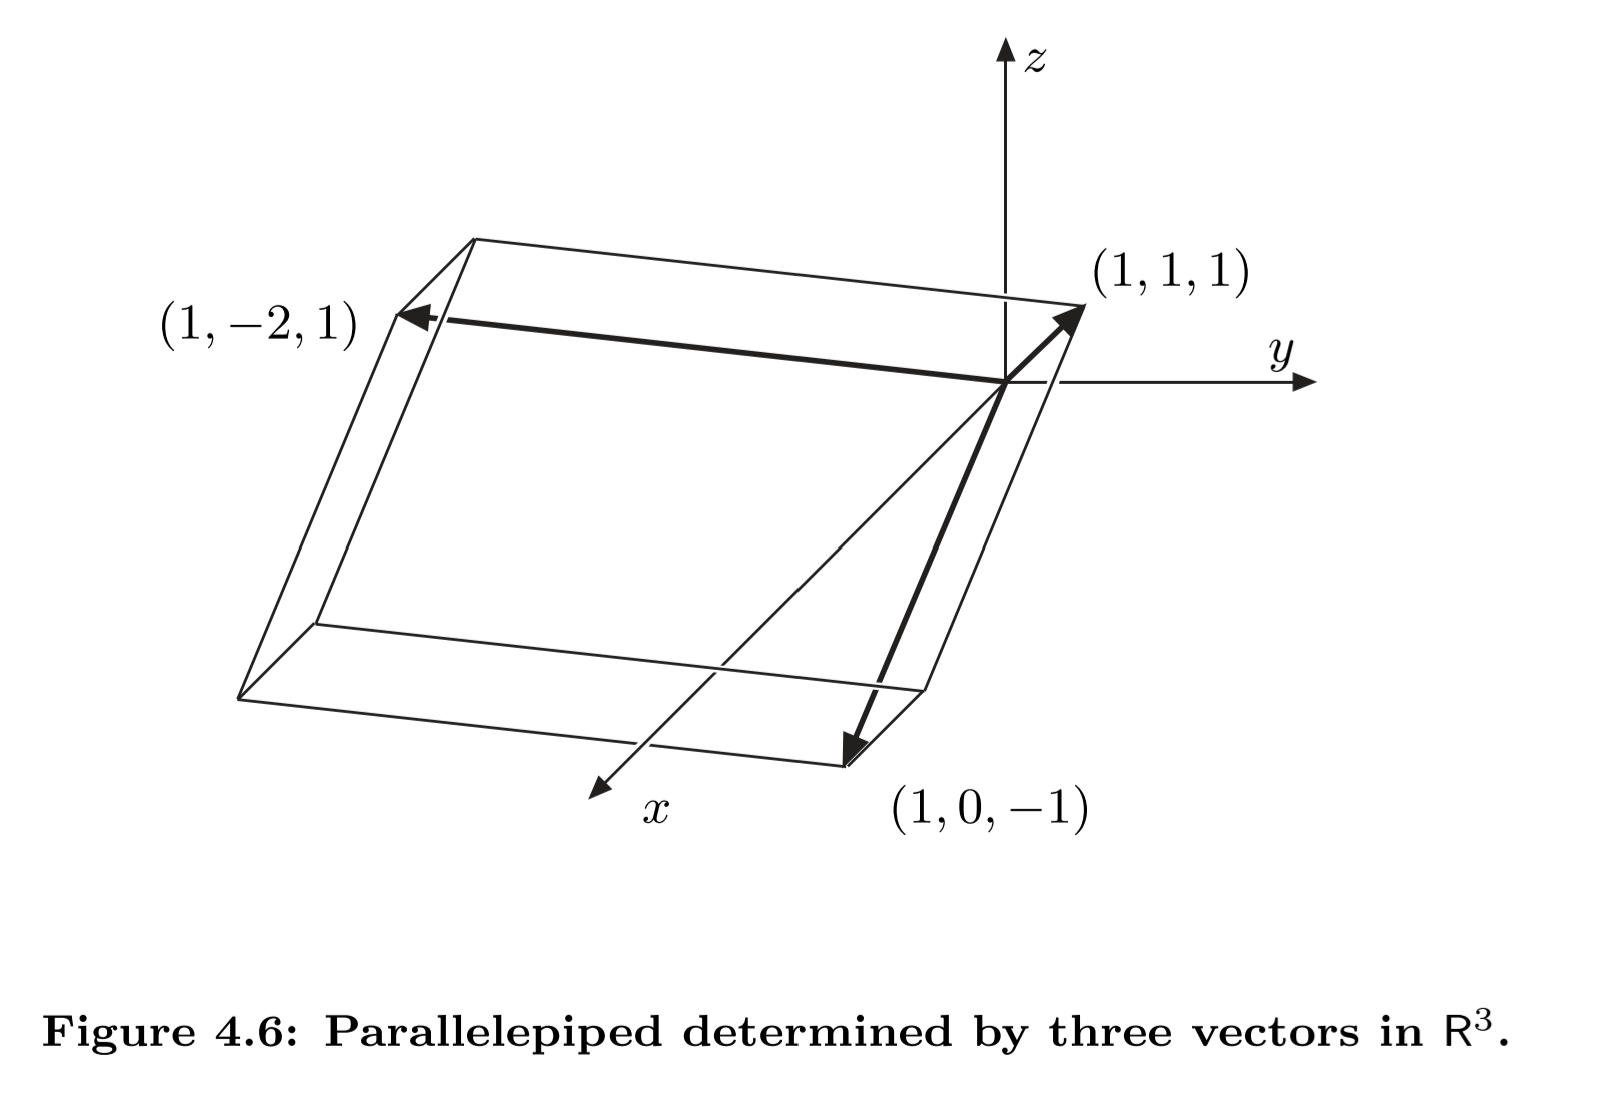
\includegraphics[width=16cm]{images/figure-4-6.png}

(BTW the figure doesn't look like a \emph{rectangular} parallelepiped.)

\begin{remark} \label{remark 4.3.4}
In our earlier discussion of the geometric significance of the determinant formed from the vectors in an ordered basis for \(\SET{R}^2\), we also saw that this determinant is positive if and only if the basis induces a \emph{right-handed coordinate system}.
(See \EXEC{4.1.13}.)
A similar statement is true in \(\SET{R}^n\).
\end{remark}

\begin{additional definition}
Specifically, if \(\gamma\) is any ordered basis for \(\SET{R}^{n}\)
and \(\beta\) is the \emph{standard} ordered basis for \(\SET{R}^n\), then \(\gamma\) induces a right-banded coordinate system if and only if \(\det(Q) > 0\), where \(Q\) is the \emph{change of coordinate matrix} that changes \(\gamma\)-coordinates into \(\beta\)-coordinates.
\end{additional definition}

Thus. for instance,
\[
    \gamma = \left\{
                \begin{pmatrix} 1 \\ 1 \\ 0 \end{pmatrix},
                \begin{pmatrix} 1 \\ -1 \\ 0 \end{pmatrix},
                \begin{pmatrix} 0 \\ 0 \\ 1 \end{pmatrix}
             \right\}
\]
induces a left-handed coordinate system in \(\SET{R}^3\) because the corresponding change of coordinate matrix (derived by \RMK{2.5.1} or \CORO{2.23.1})
\[
    \begin{pmatrix}
        1 & 1 & 0 \\
        1 & -1 & 0 \\
        0 & 0 & 1
    \end{pmatrix}
\]
has determinant \(-2 < 0\), whereas
\[
    \gamma' = \left\{
                \begin{pmatrix} 1 \\ 2 \\ 0 \end{pmatrix},
                \begin{pmatrix} -2 \\ 1 \\ 0 \end{pmatrix},
                \begin{pmatrix} 0 \\ 0 \\ 1 \end{pmatrix}
             \right\}
\]
induces a right-handed coordinate system in \(\SET{R}^3\) because the change of coordinate matrix (again derived by \RMK{2.5.1} or \CORO{2.23.1})
\[
    \begin{pmatrix}
        1 & -2 & 0 \\
        2 & 1 & 0 \\
        0 & 0 & 1
    \end{pmatrix}
\]
has determinant \(5 > 0\).

More generally, if \(\beta\) and \(\gamma\) are two ordered bases for \(\SET{R}^n\), then the coordinate systems induced by \(\beta\) and \(\alpha\) have the \emph{same orientation} (either both are right-handed or both are left-handed)
if and only if \(\det(Q) > 0\), where \(Q\) is the change of coordinate matrix that changes \(\gamma\)-coordinates into \(\beta\)-coordinates.

\exercisesection

\begin{exercise} \label{exercise 4.3.1}
Label the following statements as true or false.
\begin{enumerate}
\item If \(E\) is an elementary matrix, then \(\det(E) = \pm 1\).
\item For any \(A, B \in M_{n \X n}(F)\), \(\det(AB) = \det(A) \cdot \det(B)\).
\item A matrix \(M \in M_{n \X n}(F)\) is invertible if and only if \(\det(M) = 0\).
\item A matrix \(M \in M_{n \X n}(F)\) has rank \(n\) if and only if \(\det(M) \ne 0\).
\item For any \(A \in M_{n \X n}(F)\), \(\det(A^\top) = -\det(A)\).
\item The determinant of a square matrix can be evaluated by cofactor expansion along any \emph{column}.
\item Every system of \(n\) linear equations in \(n\) unknowns can be solved by Cramer's rule.
\item Let \(Ax = b\) be the matrix form of a system of \(n\) linear equations in \(n\) unknowns, where \(x = (x_1, x_2, ..., x_n)^\top\).
If \(\det(A) \ne 0\) and if \(M_k\) is the \(n \X n\) matrix obtained from \(A\) by replacing \RED{row} \(k\) of \(A\) by \(b^\top\), then the unique solution of \(Ax = b\) is
\[
    x_k = \cfrac{\det(M_k)}{\det(A)} \text{ for } k = 1, 2, ..., n.
\]
\end{enumerate}
\end{exercise}

\begin{proof} \ 

\begin{enumerate}
\item False. Type 2 with scalar \(c\) has determinant \(c\).
\item True by \THM{4.7}.
\item False by \CORO{4.7.1}.
\item True. \(M\) has rank \(n\), iff (by \RMK{3.2.1}) \(M\) is invertible, iff (by \CORO{4.7.1}) \(\det(M) \ne 0\).
\item False by \THM{4.8}.
\item True.
    We have \(\det(A) = \det(A^\top)\) by \THM{4.8}.
    And (by \THM{4.4}) \(\det(A^\top)\) is equal to the cofactor expansion along any \emph{row} of \(A^\top\).
    But that is equivalent to the cofactor expansion along any \(\emph{column}\) of \(A\).
\item False.
    The corresponding coefficient matrix also needs to be invertible.
\item False. By \THM{4.9}, \(M_k\) should be the \(n \X n\) matrix obtained from \(A\) by replacing \RED{column} \(k\) of \(A\) by \(b^\top\).
\end{enumerate}
\end{proof}

\begin{exercise} \label{exercise 4.3.2}
Solve the system using Cramer's rule:
\begin{align*}
    a_{11} x_1 + a_{12} x_2 & = b_1 \\
    a_{21} x_1 + a_{22} x_2 & = b_2
\end{align*}
where \(a_{11} a_{22} - a_{12} a_{21} \ne 0\).
\end{exercise}

\begin{proof}
By the given supposition, the corresponding coefficient matrix of the system
\[
    A = \begin{pmatrix} a_{11} & a_{12} \\ a_{21} & a_{22} \end{pmatrix}
\]
has nonzero determinant.
So using \THM{4.9} Cramer's rule,
\[
    M_1 = \begin{pmatrix} b_1 & a_{12} \\ b_2 & a_{22} \end{pmatrix}, \quad
    M_2 = \begin{pmatrix} a_{11} & b_1 \\ a_{21} & b_2 \end{pmatrix},
\]
and
\[
    x_1 = \cfrac{\det(M_1)}{\det(A)} = \cfrac{b_1 a_{22} - a_{12} b_2}{a_{11} a_{22} - a_{12} a_{21}},
    \quad
    x_2 = \cfrac{\det(M_2)}{\det(A)} = \cfrac{a_{11} b_2 - b_1 a_{21}}{a_{11} a_{22} - a_{12} a_{21}}
\]
\end{proof}

Exercise 3 to Exercise 7 are pure calculation problems that require solving systems using Cramer's rule. Skip.

\setcounter{exercise}{7}
\begin{exercise} \label{exercise 4.3.8}
Use \THM{4.8} to prove a result analogous to \THM{4.3}, but for columns.
\end{exercise}

\begin{proof}
Let \(A \in M_{n \X n}(F)\) such that
\[
    A = \begin{pmatrix} a_1 & a_2 & ... & a_r & ... & a_n
    \end{pmatrix},
\]
where \(a_1, ..., a_n \in F^n\) are columns of \(A\).
Now let \(a_r = u + kv\) for some \(u, v \in F^n\) and scalar \(k\), and let \(B, C\) be the same as \(A\) except for replacing row \(r\) with \(u\) and \(v\), respectively.

Then we need to show \(\det(A) = \det(B) + k \cdot \det(C)\).
Then
\begin{align*}
    \det(A) & = \det(A^\top) & \text{by \THM{4.8}} \\
            & = \det \begin{pmatrix} a_1^\top \\ \vdots \\ a_r^\top \\ \vdots \\ a_n^\top \end{pmatrix} = \det \begin{pmatrix} a_1^\top \\ \vdots \\ u^\top + k \cdot v^\top \\ \vdots \\ a_n^\top \end{pmatrix} & \text{of course} \\
            & = \det \begin{pmatrix} a_1^\top \\ \vdots \\ u^\top \\ \vdots \\ a_n^\top \end{pmatrix} + k \cdot \det \begin{pmatrix} a_1^\top \\ \vdots \\ v^\top \\ \vdots \\ a_n^\top \end{pmatrix} & \text{by \THM{4.3}} \\
            & = \det(B^\top) + k \cdot \det(C^\top) & \text{of course} \\
            & = \det(B) + k \cdot \det(C), & \text{by \THM{4.8}}
\end{align*}
as desired.
\end{proof}

\begin{exercise} \label{exercise 4.3.9}
Prove that an \emph{upper triangular} \(n \X n\) matrix is invertible if and only if all its diagonal entries are nonzero.
\end{exercise}

\begin{proof}
An \emph{upper triangular} \(n \X n\) matrix is invertible, iff (by \CORO{4.7.1}) its determinant is nonzero, iff (by \EXEC{4.2.23}) the product of its diagonal entries are nonzero, iff (of course) all its diagonal entries are nonzero.
\end{proof}

\begin{exercise} \label{exercise 4.3.10}
A matrix \(M \in M_{n \X n}(F)\) is called \href{https://www.wikiwand.com/en/Nilpotent_matrix}{nilpotent} if, for some \emph{positive} integer \(k\), \(M^k = O\), where \(O\) is the \(n \X n\) zero matrix.
Prove that if \(M\) is nilpotent, then \(\det(M) = 0\).
\end{exercise}

\begin{note}
Concept-related exercise: \EXEC{2.3.16}(b).
\end{note}

\begin{proof}
We have
\begin{align*}
             & M^k = O \\
    \implies & \det(M^k) = \det(O) = 0 & \text{of course} \\
    \implies & \det(M)^k = 0 & \text{by \THM{4.7}} \\
    \implies & \det(M) = 0 & \text{of course}
\end{align*}
\end{proof}

\begin{exercise} \label{exercise 4.3.11}
A matrix \(M \in M_{n \X n}(\SET{C})\) is called \textbf{skew-symmetric} if \(M^\top = -M\).
Prove that if \(M\) is skew-symmetric and \(n\) is odd, then \(M\) is not invertible.
What happens if \(n\) is even?
\end{exercise}

\begin{note}
The complex number has characteristic \(0 \ne 2\).
The exercise would not apply if the field of the matrix has characteristic equal to \(2\).
\end{note}

\begin{proof}
By \EXEC{4.2.25}, we have \(\det(-M) = (-1)^n \det(M)\).
And by \THM{4.8}, we have \(\det(M^\top) = \det(M)\).
And by supposition \(-M = M^\top\), so we have \((-1)^n \det(M) = \det(M)\).
If \(n\) is odd, the equation implies \(-1 \det(M) = \det(M)\).
Which implies \(\det(M) = 0 \in \SET{C}\).
If \(n\) is even, then that only implies \(\det(M) = \det(M)\), hence we cannot conclude anything.
For example, (the skew-symmetric matrix) \(\begin{pmatrix} 0 & 1 \\ -1 & 0 \end{pmatrix}\) is invertible, but (the skew-symmetric matrix) \(O_{2 \X 2}\) is not invertible.
\end{proof}

\begin{exercise} \label{exercise 4.3.12}
A matrix \(Q \in M_{n \X n}(\SET{R})\) is called \textbf{orthogonal} if \(QQ^\top = I\).
Prove that if \(Q\) is orthogonal, then \(\det(Q) = \pm 1\).
\end{exercise}

\begin{note}
This exercise should be related to \CH{6}.
\end{note}

\begin{proof}
We have
\begin{align*}
    1 = \det(I) & = \det(QQ^\top) & \text{by supposition} \\
                & = \det(Q) \det(Q^\top) & \text{by \THM{4.7}} \\
                & = \det(Q) \det(Q), & \text{by \THM{4.8}} \\
\end{align*}
which implies \(\det(Q) = \pm 1\).
\end{proof}

\begin{exercise} \label{exercise 4.3.13}
For \(M \in M_{n \X n}(\SET{C})\), let \(\conjugatet{M}\) be the matrix such that \((\conjugatet{M})_{ij} = \conjugatet{M_{ij}}\) for all \(i, j\),
where \(\conjugatet{M_{ij}}\) is the complex conjugate of \(M_{ij}\).
\begin{enumerate}
\item Prove that \(\det(\conjugatet{M}) = \conjugatet{\det(M)}\).

\item A matrix \(Q \in M_{n \X n}(\SET{C})\) is called \textbf{unitary} if \(QQ^* = I\), where \(Q^* = \conjugatet{Q^\top}\).
Prove that if \(Q\) is a \emph{unitary} matrix, then \(\left| \det(Q) \right| = 1\).
\end{enumerate}
\end{exercise}

\begin{proof} \ 

\begin{enumerate}
\item We prove by induction on \(n\).
For \(n = 1\),
\begin{align*}
    \det(\conjugatet{M}) & = (\conjugatet{M})_{11} & \text{by \DEF{4.2} for dimension \(= 1\)} \\
                         & = \conjugatet{M_{11}} & \text{by supposition} \\
                         & = \conjugatet{\det(M)} & \text{by \DEF{4.2} for dimension \(= 1\)}
\end{align*}

Suppose inductively \(\det(\conjugatet{M}) = \conjugatet{\det(M)}\) for arbitrary \(M \in M_{k \X k}(\SET{C})\) such that \((\conjugatet{M})_{ij} = \conjugatet{M_{ij}}\) for all \(i, j\).
We have to show \(\det(\conjugatet{M}) = \conjugatet{\det(M)}\) for arbitrary \(M \in M_{(k + 1) \X (k + 1)}(\SET{C})\) such that \((\conjugatet{M})_{ij} = \conjugatet{M_{ij}}\) for all \(i, j\).
Then
\begin{align*}
    \det(\conjugatet{M}) & = \sum_{j = 1}^{(k + 1)} (\conjugatet{M})_{1j} \cdot (-1)^{1 + j} \cdot \det(\widetilde{(\conjugatet{M})}_{1j}) & \text{by \DEF{4.2}} \\
                         & = \sum_{j = 1}^{(k + 1)} \RED{\conjugatet{M_{1j}}} \cdot (-1)^{1 + j} \cdot \det(\widetilde{(\conjugatet{M})}_{1j}) & \text{by supposition} \\
                         & = \sum_{j = 1}^{(k + 1)} \conjugatet{M_{1j}} \cdot (-1)^{1 + j} \cdot \RED{\conjugatet{\det(\tilde{M}_{1j})}} & \text{by inductive hypothesis} \\
                         & = \sum_{j = 1}^{(k + 1)} \conjugatet{M_{1j} \cdot (-1)^{1 + j}} \cdot \conjugatet{\det(\tilde{M}_{1j})} & \text{of course (see theorem D.2(c)(e))} \\
                         & = \sum_{j = 1}^{(k + 1)} \conjugatet{M_{1j} \cdot (-1)^{1 + j} \cdot \det(\tilde{M}_{1j})} & \text{of course (see theorem D.2)(c)} \\
                         \\
                         & = \conjugatet{\sum_{j = 1}^{(k + 1)} M_{1j} \cdot (-1)^{1 + j} \cdot \det(\tilde{M}_{1j})} & \text{of course (see theorem D.2)(b)} \\
                         & = \conjugatet{\det(M)} & \text{by \DEF{4.2}}
\end{align*}

\item We have
\begin{align*}
    1 = \det(I) & = \det(QQ^*) & \text{by supposition} \\
                & = \det(Q) \det(Q^*) & \text{by \THM{4.7}} \\
                & = \det(Q) \det(\conjugatet{Q^\top}) & \text{by definition} \\
                & = \det(Q) \conjugatet{\det(Q^\top)} & \text{by part(a)} \\
                & = \det(Q) \conjugatet{\det(Q)} & \text{by \THM{4.8}} \\
                & = \abs{\det(Q)}^2, & \text{by definition in page 551}
\end{align*}
which implies \(\abs{\det(Q)} = 1\).
\end{enumerate}
\end{proof}

\begin{exercise} \label{exercise 4.3.14}
Let \(\beta = \{ u_1, u_2, ..., u_n \}\) be a subset of \(F^n\) containing \(n\) distinct vectors, and let \(B\) be the matrix in \(M_{n \X n}(F)\) having \(u_j\) as column \(j\).
Prove that \(\beta\) is a basis for \(F^n\) if and only if \(\det(B) \ne 0\).
\end{exercise}

\begin{proof}
We have \(\beta\) is a basis for \(F^n\) iff (by \CH{3}) \(\rank(B) = n\), iff (by \EXEC{4.3.1}(d)) \(\det(B) \ne 0\).
\end{proof}

\begin{exercise} \label{exercise 4.3.15}
Prove that if \(A, B \in M_{n \X n}(F)\) are \emph{similar}, then \(\det(A) = \det(B)\).
\end{exercise}

\begin{proof}
If \(A, B \in M_{n \X n}(F)\) are similar, then by \DEF{2.16} we have \(B = Q^{-1} A Q\) for some invertible \(Q\).
And
\begin{align*}
    \det(B) & = \det(Q^{-1} A Q) \\
            & = \det(Q^{-1}) \det(A) \det(Q) & \text{by \THM{4.7}} \\
            & = \det(Q^{-1}) \det(Q) \det(A) & \text{of course} \\
            & = \det(Q^{-1} Q) \det(A) & \text{by \THM{4.7}} \\
            & = \det(I) \det(A) & \text{of course} \\
            & = 1 \cdot \det(A) = \det(A) & \text{of course}
\end{align*}
\end{proof}

\begin{exercise} \label{exercise 4.3.16}
Use determinants to prove that if \(A, B \in M_{n \X n}(F)\) are such that \(AB = I\), then \(A\) is invertible (and hence \(B = A^{-1}\)).
\end{exercise}

\begin{note}
This is related to \ATHM{2.38}.
\end{note}

\begin{proof}
We have
\begin{align*}
    1 = \det(I) & = \det(AB) & \text{by supposition} \\
                & = \det(A) \det(B), & \text{by \THM{4.7}}
\end{align*}
which implies both \(\det(A)\) and \(\det(B)\) cannot be zero.
And in particular by \CORO{4.7.1}, \(A\) is invertible.
And by \ATHM{2.38}(1), \(B = A^{-1}\).
\end{proof}

\begin{exercise} \label{exercise 4.3.17}
Let \(A, B \in M_{n \X n}(F)\) be such that \(AB = -BA\).
Prove that if \(n\) is odd and \(F\) is \emph{not} a field of characteristic two, then \(A\) or \(B\) is not invertible.
\end{exercise}

\begin{proof}
We have
\begin{align*}
    \det(A) \det(B) & = \det(AB) & \text{by \THM{4.7}} \\
                    & = \det(-BA) & \text{by supposition} \\
                    & = (-1)^n \cdot \det(BA) & \text{by \EXEC{4.2.25}} \\
                    & = (-1) \cdot \det(BA) & \text{since \(n\) is odd} \\
                    & = -1 \cdot \det(B) \det(A) & \text{by \THM{4.7}} \\
                    & = -1 \cdot \det(A) \det(B) & \text{of course} \\
    \implies 2 \cdot \det(A) \det(B) = 0.
\end{align*}
Since \(F\) is \emph{not} a field of characteristic two, that implies \(\det(A) \det(B) = 0\), so \(\det(A)\) \emph{or} \(\det(B)\) is zero, so by \CORO{4.7.1}, \(A\) or \(B\) is not invertible.
\end{proof}

\begin{exercise} \label{exercise 4.3.18}
Complete the proof of \THM{4.7} by showing that if \(A\) is an \emph{elementary matrix} of type 2 or type 3, then \(\det(AB) = \det(A) \cdot \det(B)\).
\end{exercise}

\begin{proof}
If \(A\) is type 2, then \(A\) has the form
\[
    A = \begin{pmatrix}
        e_1 \\ e_2 \\ \vdots \\ k e_i \\ \vdots \\ e_n
    \end{pmatrix}
\]
where \(k\) is nonzero scalar.
And by \THM{3.1}, \(AB\) is equal to \(B\) with row \(i\) multiplied by \(k\), so by \RMK{4.2.3}(b), \(\det(AB) = k \cdot \det(B)\) \MAROON{(1)}.
And by \RMK{4.3.1}, \(\det(A) = k\), hence by \MAROON{(1)} we have \(\det(AB) = \det(A) \cdot \det(B)\).

If \(A\) is type 3, then \(A\) has the form
\[
    A = \begin{pmatrix}
        e_1 \\ e_2 \\ \vdots \\ k e_i + e_j \\ \vdots \\ e_n
    \end{pmatrix}
\]
And by \THM{3.1}, \(AB\) is equal to \(B\) but adding \(k\) times row \(i\) to row \(j\), so by \RMK{4.2.3}(c), \(\det(AB) = \det(B)\) \MAROON{(2)}.
And by \RMK{4.3.1}, \(\det(A) = 1\), hence by \MAROON{(2)} we have \(\det(AB) = \det(B) = 1 \cdot \det(B) = \det(A) \cdot \det(B)\).
\end{proof}

\begin{exercise} \label{exercise 4.3.19}
A matrix \(A \in M_{n \X n}(F)\) is called \textbf{lower triangular} if \(A_{ij} = 0\) for \(1 \le i < j \le n\).
Suppose that \(A\) is a lower triangular matrix.
Describe \(\det(A)\) in terms of the entries of \(A\).
\end{exercise}

\begin{proof}
If \(A\) is lower triangular, then \(A^\top\) is upper triangular.
By \THM{4.8}, \(\det(A) = \det(A^\top)\).
And by \EXEC{4.2.23}, we know \(\det(A^\top)\) is equal to the product of its diagonals, so \(\det(A)\) is equal to the product of \(A^\top\)'s diagonals.
But \(A^\top\)'s diagonals are of course \(A\)'s diagonals, so \(\det(A)\) is also equal to the product of its diagonals.
\end{proof}

\begin{exercise} \label{exercise 4.3.20}
Suppose that \(M \in M_{n \X n}(F)\) can be written in the form
\[
    M = \begin{pmatrix} A & B \\ O & I \end{pmatrix},
\]
where \(A\) is a \emph{square} matrix.
Prove that \(\det(M) = \det(A)\).
\end{exercise}

\begin{proof}
Informally, if we expand the last row of \(M\), then ultimately we have
\[
    \det(M) = 1 \cdot 1 \cdot ... \cdot 1 \cdot \det(A) = \det(A).
\]
\end{proof}

\begin{exercise} \label{exercise 4.3.21}
Prove that if \(M \in M_{n \X n}(F)\) can be written in the form
\[
    M = \begin{pmatrix} A & B \\ O & C \end{pmatrix},
\]
where \(A\) and \(C\) are square matrices, then \(\det(M) = \det(A) \cdot \det(C)\).
\end{exercise}

\begin{proof}
There are two cases: \(C\) is invertible or not.

If \(C\) is not invertible, then the rows of \(C\) is \emph{not} \LID{}, and (by \CORO{4.7.1}) \(\det(C) = 0\);
and of course the rows of \((O|C)\) is not \LID{}, which implies \(M\) has rank less then \(n\), so (by \CORO{4.6.1}) \(\det(M) = 0\).
And \(\det(A) \cdot \det(C) = \det(A) \cdot 0 = 0\), hence \(\det(M) = \det(A) \cdot \det(C)\).

If \(C\) is invertible, then given the matrix
\[
    M' = \begin{pmatrix} I & O \\ O & C^{-1} \end{pmatrix},
    M'' = \begin{pmatrix} A & B \\ O & I \end{pmatrix},
\]
by (the generalization of) \ATHM{3.7},
\[
    M' M =
    \begin{pmatrix} I & O \\ O & C^{-1} \end{pmatrix}
    \begin{pmatrix} A & B \\ O & C \end{pmatrix}
    = M'',
\]
So we have \(\det(M' M) = \det(M'')\), so by \THM{4.7}, \(\det(M')\det(M) = \det(M'')\) \MAROON{(1)}.
By (similar argument of) \EXEC{4.3.20}, \(\det(M') = \det(C^{-1})\).
And by \EXEC{4.3.20}, \(\det(M'') = \det(A)\), so by \MAROON{(1)}, we have \(\det(C^{-1}) \det(M) = \det(A)\).
And by \CORO{4.7.1}, that implies
\[
    \cfrac{1}{\det(C)} \det(M) = \det(A), \text{ so } \det(M) = \det(A) \cdot \det(C).
\]
So in all cases, we have \(\det(M) = \det(A) \cdot \det(C)\).
\end{proof}

\begin{exercise} \label{exercise 4.3.22}
Let \(\T : \POLYNF \to F^{n + 1}\) be the \LTRAN{} defined in \EXEC{2.4.22} by \(\T(f) = (f(c_0), f(c_1), ..., f(c_n))\), where \(c_0, c_1, ..., c_n\) are \emph{distinct} scalars in an infinite field \(F\).
Let \(\beta\) be the \emph{standard} ordered basis for \(\POLYNF\) and \(\gamma\) be the \emph{standard} ordered basis for \(F^{n + 1}\).
\begin{enumerate}
\item Show that the \((n + 1) \X (n + 1)\) matrix \(M = [\T]_{\beta}^{\gamma}\) has the form
\[
    \begin{pmatrix}
        1 & c_0 & c_0^2 & ... & c_0^n \\\
        \vdots & \vdots & \vdots & & \vdots \\
        1 & c_{n-1} & c_{n-1}^2 & ... & c_{n-1}^n \\
        1 & c_n & c_n^2 & ... & c_n^n
    \end{pmatrix}
\]
A matrix with this form is called a \textbf{Vandermonde matrix}.
\item Use \EXEC{2.4.22} to prove that \(\det(M) \ne 0\).
\item Prove that
\[
    \det(M) = \prod_{0 \le i < j \le n} (c_j - c_i),
\]
the product of all terms of the form \(c_j - c_i\) for \(0 \le i < j \le n\).
\end{enumerate}
\end{exercise}

\begin{proof} \ 

\begin{enumerate}
\item
For the standard ordered base \(\beta = \{ 1, x, x^2, ..., x^n \}\), we have
\begin{align*}
    \T(1) & = (1, 1, ..., 1) = 1 \cdot e_1 + 1 \cdot e_2 + ... + 1 \cdot e_{n+1} \\
    \T(x) & = (c_0, c_1, ..., c_n) = c_0 \cdot e_1 + c_1 \cdot e_2 + ... + c_n \cdot e_{n+1} \\
    \T(x^2) & = (c_0^2, c_1^2, ..., c_n^2) = c_0^2 \cdot e_1 + c_1^2 \cdot e_2 + ... + c_n^2 \cdot e_{n+1} \\
    \vdots \\
    \T(x^n) & = (c_0^n, c_1^n, ..., c_n^n) = c_0^n \cdot e_1 + c_1^n \cdot e_2 + ... + c_n^n \cdot e_{n+1}
\end{align*}
So \([\T]_{\beta}^{\gamma}\) has that desired form.

\item \(\T\) is an isomorphism, so by \THM{2.18}, \(M = [\T]_{\beta}^{\gamma}\) is invertible, so by \CORO{4.7.1}, \(\det(M) \ne 0\).

\item Let
\[
    F_1 = \begin{pmatrix}
        1 & c_0 & c_0^2 & ... & c_0^n \\\
        \vdots & \vdots & \vdots & & \vdots \\
        1 & c_{n-1} & c_{n-1}^2 & ... & c_{n-1}^n \\
        1 & x & x^2 & ... & x^n
    \end{pmatrix}
    \quad \text{and } \quad
    f_1(x) = \det (F_1).
\]
Then its clear that, by expanding the last row of \(F_1\), \(f_1(x)\) is a polynomial of degree \(n\).
And in particular,
\[
    f_1(c_n) = \det(M) \quad \quad \MAROON{(1.1)}.
\]
Furthermore, \(c_0, c_1, ..., c_{n-1}\) are the \(n\) roots of this polynomial, since from the structure of \(F_1\), if we replace \(x\) with \(c_0, ..., c_{n - 1}\), then \(F_1\) has two identical rows, so (by \CORO{4.4.1}) the determinant is equal to zero.
So \(f_1(x)\) has the form
\[
    f_1(x) = \alpha_1 (x - c_0)(x - c_1) ... (x - c_{n - 1}), \quad \quad \MAROON{(1.2)}
\]
where \(\alpha_1\) is a nonzero scalar.
\textbf{But again}, from the structure of \(F_1\), \(\alpha_1\) is in fact equal to the cofactor of the row \(n + 1\), column \(n + 1\).
That is,
\[
    \alpha_1 = (-1)^{(n + 1) + (n + 1)} \det \left( \widetilde{F_1}_{(n+1)(n+1)} \right) = \det\left( \widetilde{F_1}_{(n+1)(n+1)} \right).
\]
\emph{That is},
\[
    \alpha_1 = \det \begin{pmatrix}
        1 & c_0 & c_0^2 & ... & c_0^{n \RED{- 1}} \\\
        \vdots & \vdots & \vdots & & \vdots \\
        1 & c_{n \RED{-1}} & c_{n \RED{-1}}^2 & ... & c_{n \RED{-1}}^{n \RED{- 1}}
    \end{pmatrix}. \quad \quad \MAROON{(1.3)}
\]
Now if we \textbf{use the same argument again}, then we let
\[
    F_2 = \begin{pmatrix}
        1 & c_0 & c_0^2 & ... & c_0^{n - 1} \\\
        \vdots & \vdots & \vdots & & \vdots \\
        1 & c_{n-2} & c_{n-2}^2 & ... & c_{n-2}^{n - 1} \\
        1 & x & x^2 & ... & x^{n-1}
    \end{pmatrix}
    \quad \text{and} \quad
    f_2(x) = \det(F_2).
\]
Then in particular, by observation,
\[
    f_2(c_{n - 1}) = \alpha_1 \quad \quad \MAROON{(2.1)}.
\]
Using the same argument, we have
\[
    f_2(x) = \alpha_2 (x - c_0)(x - c_1) ... (x - c_{n - 2}), \quad \quad \MAROON{(2.2)}
\]
where
\[
    \alpha_2 = \det \begin{pmatrix}
        1 & c_0 & c_0^2 & ... & c_0^{n \RED{- 2}} \\\
        \vdots & \vdots & \vdots & & \vdots \\
        1 & c_{n \RED{-2}} & c_{n \RED{-2}}^2 & ... & c_{n \RED{-2}}^{n \RED{- 2}}
    \end{pmatrix}. \quad \quad \MAROON{(2.3)}
\]

Continue this process \emph{inductively}, we have
\begin{align*}
    \det(M) & = f_1(c_n) & \text{by \MAROON{(1.1)}} \\
            & = \alpha_1 \cdot (c_n - c_0) (c_n - c_1) ... (c_n - c_{n - 1}) & \text{by \MAROON{(1.2)}} \\
            & = f_2(c_{n - 1}) \cdot [(c_n - c_0) (c_n - c_1) ... (c_n - c_{n - 1})] & \text{by \MAROON{(2.1)}} \\
            & = \big[ \alpha_2 (c_{n - 1} - c_0) (c_{n - 1} - c_1) ... (c_{n - 1} - c_{n - 2}) \big] \\
            & \quad \quad \cdot \big[ (c_n - c_0) (c_n - c_1) ... (c_n - c_{n - 1}) \big] & \text{by \MAROON{(2.2)}} \\
            & \quad \vdots \\
            & = \big[(c_1 - c_0)] \big[(c_2 - c_0) (c_2 - c_1) ] \\
            & \quad \quad \cdot ... \\
            & \quad \quad \cdot \big[ (c_{n - 1} - c_0) (c_{n - 1} - c_1) ... (c_{n - 1} - c_{n - 2}) \big] \\
            & \quad \quad \cdot \big[ (c_n - c_0) (c_n - c_1) ... (c_n - c_{n - 1}) \big] & \text{expand inductively} \\
            & = \prod_{0 \le i < j \le n} (c_j - c_i).
\end{align*}
\end{enumerate}
\end{proof}

\begin{exercise} \label{exercise 4.3.23}
Let \(A \in M_{n \X n}(F)\) be nonzero.
For any \(m\) (\(1 \le m \le n\)), an \(m \X m\) \textbf{submatrix} is obtained by deleting \emph{any} \(n - m\) rows and any \(n - m\) columns of \(A\).
(The concept is similar to a \emph{subsequence} of a sequence.)
\begin{enumerate}
\item Let \(k\) (\(1 \le k \le n\)) denote the \emph{largest} integer such that some \(k \X k\) submatrix has a nonzero determinant.
Prove that \(\rank(A) = k\).
\item Conversely, suppose that \(\rank(A) = k\).
Prove that there exists a \(k \X k\) submatrix with a nonzero determinant.
\end{enumerate}
\end{exercise}

\begin{proof} \ 

\begin{enumerate}
\item
If \(\rank(A) = n\), that means \(A\) is invertible, and by \CORO{4.7.1}, \(\det(A) \ne 0\).
So the largest submatrix with a nonzero determinant is \(A\) itself, which has size \(n \X n\), so in this case, \(k = n\), which is equal to \(\rank(A)\).

Now suppose \(\rank(A) < n\).
We will show that \(\rank(A) < k\) and \(\rank(A) > k\) lead to contradiction.

So for the sake of contradiction, suppose
\[
    \rank(A) < k. \quad \quad \BLUE{(1)}
\]
First let \(B\) be the \(k \X k\) submatrix of \(A\) with nonzero determinant.
Then by \CORO{4.7.1}, \(B\) is invertible, and the columns \(S = \{ v_1, v_2, ..., v_k \}\) of \(B\) are \LID{}.
Now consider the \(k \X \RED{n}\) submatrix \(C\) of \(A\) obtained by deleting those rows who were deleted when we construct \(B\).
Then \(S\) is a \emph{subset} of the columns of \(C\).
This means \(\rank(C) \ge \#S = k\).
But by \THM{3.6}, \(\rank(C) \le \min(k, n) = k\).
Hence \(\rank(C) = k\), which implies the \(k\) rows of \(C\) are also \LID{}.
And thus the matrix \(A\) contains these \(k\) \LID{} rows and hence \(\rank(A) \ge k\), which contradicts \BLUE{(1)}.

Now, for the sake of contradiction, suppose
\[
    \rank(A) > k. \quad \quad \BLUE{(2)}
\]
Let \(\rank(A) = r\).
Then we can pick \(r\) \LID{} rows of \(A\), say \(u_1, ..., u_r\), to construct a \(r \X n\) submatrix \(D\) of \(A\).
Then \(D\) has \(\rank(D) \ge r\).
And by \THM{3.6}, \(\rank(D) \le \min(r, n) = r\), hence \(\rank(D) = r\).
Now we can also pick \(r\) \LID{} \emph{columns}, say \(v_1, ..., v_r\), of \(D\), to construct an \(r \X r\) submatrix \(D'\) of \(D\).
Note that \(D'\) is also a submatrix of \(A\).
Then \(\rank(D') \ge r\), and again by \THM{3.6}, \(\rank(D') \le min(r, r) = r\), hence \(\rank(D') = r\).
This implies \(D'\) is invertible, and by \CORO{4.7.1}, \(\det(D') \ne 0\).
So we have found a \(r \X r\) submatrix of \(A\) with nonzero determinant and \(r > k\), which contradicts the property of \(k\) that \(k\) is the size of the ``largest'' nonzero determinant submatrix of \(A\).

So \(\rank(A)\) must be equal to \(k\).

\item This is similar to the second part of the proof in part(a),
We just pick \(k\) \LID{} rows of \(A\) to construct a \(k \X n\) submatrix, and pick \LID{} \(k\) columns of that submatrix to construct a \(k \X k\) submatrix.
Then such \(k \X k\) matrix is a submatrix of \(A\) and has nonzero determinant.
\end{enumerate}
\end{proof}

\begin{exercise} \label{exercise 4.3.24}
Let \(A \in M_{n \X n}(F)\) have the form
\[
    A = \left(\begin{array}{rrcccc}
        0 & 0 & 0 & \cdots & 0 & a_{0} \\
        -1 & 0 & 0 & \cdots & 0 & a_{1} \\
        0 & -1 & 0 & \cdots & 0 & a_{2} \\
        \vdots & \vdots & \vdots & \ddots & \vdots & \vdots \\
        0 & 0 & 0 & \cdots & 0 & a_{n-2} \\
        0 & 0 & 0 & \cdots & -1 & a_{n-1}
    \end{array}\right)
\]
Compute \(\det(A + tI)\), where \(I\) is the \(n \X n\) identity matrix.
\end{exercise}

\begin{proof}
\(A + tI\) has the form
\[
    \begin{pmatrix}
        t      & 0      & 0      & \cdots & 0      & a_{0} \\
        -1     & t      & 0      & \cdots & 0      & a_{1} \\
        0      & -1     & t      & \cdots & 0      & a_{2} \\
        \vdots & \vdots & \vdots & \ddots & \vdots & \vdots \\
        0      & 0      & 0      & \cdots & t      & a_{n-2} \\
        0      & 0      & 0      & \cdots & -1     & t + a_{n-1}
    \end{pmatrix}
\]
We perform type 3 elementary row operations:
\begin{align*}
    \begin{pmatrix}
        t      & 0      & 0      & \cdots & 0      & a_{0} \\
        -1     & t      & 0      & \cdots & 0      & a_{1} \\
        0      & -1     & t      & \cdots & 0      & a_{2} \\
        \vdots & \vdots & \vdots & \ddots & \vdots & \vdots \\
        0      & 0      & 0      & \cdots & t      & a_{n-2} \\
        0      & 0      & 0      & \cdots & -1     & t + a_{n-1}  
    \end{pmatrix}
    \to
    \begin{pmatrix}
        t       & 0      & 0      & \cdots & 0      & a_{0} \\
        \RED{0} & t      & 0      & \cdots & 0      & \RED{a_{1} + \cfrac{a_0}{t}} \\
        0       & -1     & t      & \cdots & 0      & a_{2} \\
        \vdots  & \vdots & \vdots & \ddots & \vdots & \vdots \\
        0      & 0      & 0      & \cdots & t      & a_{n-2} \\
        0       & 0      & 0      & \cdots & -1     & t + a_{n-1}  
    \end{pmatrix} \\
    \to
    \begin{pmatrix}
        t       & 0       & 0      & \cdots & 0      & a_{0} \\
        0       & t       & 0      & \cdots & 0      & a_{1} + \cfrac{a_0}{t} \\
        0       & \RED{0} & t      & \cdots & 0      & \RED{a_{2} + \cfrac{a_{1}}{t} + \cfrac{a_0}{t^2}} \\
        \vdots  & \vdots  & \vdots & \ddots & \vdots & \vdots \\
        0       & 0       & 0      & \cdots & t      & a_{n-2} \\
        0       & 0       & 0      & \cdots & -1     & t + a_{n-1}   
    \end{pmatrix}
    \to ... \to
    \begin{pmatrix}
        t       & 0       & 0      & \cdots & 0       & a_{0} \\
        0       & t       & 0      & \cdots & 0       & a_{1} + \cfrac{a_0}{t} \\
        0       & 0       & t      & \cdots & 0       & a_{2} + \cfrac{a_{1}}{t} + \cfrac{a_0}{t^2} \\
        \vdots  & \vdots  & \vdots & \ddots & \vdots  & \vdots \\
        0       & 0       & 0      & \cdots & t       & \vdots \\
        0       & 0       & 0      & \cdots & \RED{0} & \RED{t + a_{n-1} + \cfrac{a_{n-2}}{t} + ... + \cfrac{a_0}{t^{n-1}}}
    \end{pmatrix}
\end{align*}
which is upper triangular.
So by \EXEC{4.2.23}, the determinant is equal to the product of the diagonal entries, that is
\[
    t^{n - 1} (t + a_{n-1} + \cfrac{a_{n-2}}{t} + ... + \cfrac{a_0}{t^{n-1}})
    = t^n + t^{n - 1} a_{n - 1} + t^{n - 2} a_{n - 2} + ... + t a_1 + a_0.
\]
So \(\det(A) = t^n + t^{n - 1} a_{n - 1} + t^{n - 2} a_{n - 2} + ... + t a_1 + a_0\).
\end{proof}

\begin{exercise} \label{exercise 4.3.25}
Let \(c_{jk}\) denote the cofactor (see \DEF{4.2}) of the row \(j\), column \(k\) entry of the matrix \(A \in M_{n \X n}(F)\).
\begin{enumerate}
\item Prove that if \(B\) is the matrix obtained from \(A\) by replacing \emph{column} \(k\) by \(e_j\), then \(\det(B) = c_{jk}\).

\item Show that for \(1 \le j \le n\), we have
\[
    A \begin{pmatrix} c_{j1} \\ c_{j2} \\ \vdots \\ c_{jn} \end{pmatrix}
    = \det(A) \cdot e_j.
\]
Hint: Apply Cramer's rule to \(Ax = e_j\).

\item Deduce that if \(C\) is the \(n \X n\) matrix such that \(C_{ij} = c_{\RED{ji}}\), then \(AC = [\det(A)]I\).
(Notice the order of the suffix.)

\item Show that if \(\det(A) \ne 0\), then \(A^{-1} = [\det(A)]^{-1}C\).
\end{enumerate}
\end{exercise}

\begin{proof} \ 

\begin{enumerate}
\item Just expanding the column \(k\) of \(B\):
\begin{align*}
    \det(B) & = \sum_{i = 1}^n B_{ik} \cdot (-1)^{i + k} \det(\tilde{B}_{ik}) \\
            & = \sum_{i = 1}^n A_{ik} \cdot (-1)^{i + k} \det(\tilde{B}_{ik}) & \text{since \(A, B\) only differ in column \(k\)} \\
            & = \sum_{i = 1}^n B_{ik} \cdot c_{ik} & \text{by def of cofactor} \\
            & = 0 \cdot c_{1k} + ... + 1 \cdot c_{jk} + ... + 0 \cdot c_{nk} & \text{since column \(k\) of \(B = e_j\)} \\
            & = c_{jk}.
\end{align*}

\item We just check each entry of the product.
The product is
\begin{equation} \label{exec.4.3.25.eq}
    A \begin{pmatrix} c_{j1} \\ c_{j2} \\ \vdots \\ c_{jn} \end{pmatrix}
    = \begin{pmatrix}
        A_{11} c_{j1} + ... + A_{1n} c_{jn} \\
        A_{21} c_{j1} + ... + A_{2n} c_{jn} \\
        \vdots \\
        \RED{A_{j1} c_{j1} + ... + A_{jn} c_{jn}} \\
        \vdots \\
        A_{n1} c_{j1} + ... + A_{nn} c_{jn}
    \end{pmatrix}
    = \begin{pmatrix}
        \sum_{k = 1}^n A_{1k} c_{jk} \\
        \sum_{k = 1}^n A_{2k} c_{jk} \\
        \vdots \\
        \RED{\det(A)} \\
        \vdots \\
        \sum_{k = 1}^n A_{nk} c_{jk}
    \end{pmatrix}
\end{equation}
For the \(i\)th entry of the product where \(i \ne j\), it can be seen as the cofactor expansion of \(B_i\) that is obtained by replacing the \(j\)th row of \(A\) with the \(i\)th row of \(A\);
that is,
\[
    B_i = \begin{blockarray}{cccc}
        \begin{block}{(ccc)c}
        A_{11} & ... & A_{1n} & \\
        \vdots &     & \vdots & \\
        A_{i1} & ... & A_{in} & \RED{i} \\
        \vdots &     & \vdots & \\
        \RED{A_{i1}} & \RED{...} & \RED{A_{in}} & \RED{j}\\
        \vdots &     & \vdots & \\
        A_{n1} & ... & A_{nn} & \\
        \end{block}
    \end{blockarray}
\]
Since \(B_i\) has two identical rows, by \CORO{4.4.1}, \(\det(B_i) = 0\);
that is, the \(i\)th entry, where \(i \ne j\), of the product in \ref{exec.4.3.25.eq} is zero.
Hence
\[
    A \begin{pmatrix} c_{j1} \\ c_{j2} \\ \vdots \\ c_{jn} \end{pmatrix} = \begin{pmatrix}
        0 \\ \vdots \\ \det(A) \\ \vdots \\ 0
    \end{pmatrix} = \det(A) \cdot e_j.
\]

\item By the previous exercise
\begin{align*}
    AC & = A \begin{pmatrix}
            c_{11} & c_{21} & ... & c_{n1} \\
            c_{12} & c_{22} & ... & c_{n2} \\
            \vdots & \vdots &     & \vdots \\
            c_{1n} & c_{2n} & ... & c_{nn}
           \end{pmatrix} \\
       & = \begin{pmatrix}
           A \begin{pmatrix} c_{11} \\ c_{12} \\ \vdots \\ c_{1n} \end{pmatrix}
           & A \begin{pmatrix} c_{21} \\ c_{22} \\ \vdots \\ c_{2n} \end{pmatrix}
           & ...
           & A \begin{pmatrix} c_{n1} \\ c_{n2} \\ \vdots \\ c_{nn} \end{pmatrix}
       \end{pmatrix} & \text{by \THM{2.13}(a)} \\
       & = \begin{pmatrix}
           \det(A) e_1 & \det(A) e_2 & ... & \det(A) e_n
       \end{pmatrix} & \text{by part(b)} \\
       & = \det(A) \begin{pmatrix} e_1 & e_2 & ... & e_n \end{pmatrix} = \det(A) \cdot I & \text{of course}
\end{align*}
In fact the matrix \(C\) is called the classical adjoint matrix of \(A\), see \ADEF{4.4} below.

\item If \(\det(A) \ne 0\), then by \CORO{4.7.1}, \(A\) is invertible.
And
\begin{align*}
             & AC = \det(A) \cdot I & \text{by part(c)} \\
    \implies & A^{-1} AC = A^{-1} (\det(A) \cdot I) \\
    \implies & C = \det(A) \cdot A^{-1} I \\
    \implies & C = \det(A) \cdot A^{-1} \\
    \implies & [\det(A)]^{-1} C = A^{-1}
\end{align*}
\end{enumerate}
\end{proof}

\begin{additional definition} \label{adef 4.4}
The \textbf{classical adjoint} of a square matrix \(A\) is the \emph{transpose} of the matrix whose \(ij\)-entry is the \(ij\)-cofactor of \(A\).
That is, the \(ij\)-entry of the classical adjoint is the \(ji\)-cofactor of \(A\).
\end{additional definition}

\begin{exercise} \label{exercise 4.3.26}
Find the classical adjoint of each of the following matrices.

(a) \(\left(\begin{array}{ll}A_{11} & A_{12} \\ A_{21} & A_{22}\end{array}\right)\)
(b) \(\left(\begin{array}{lll}4 & 0 & 0 \\ 0 & 4 & 0 \\ 0 & 0 & 4\end{array}\right)\)

(c) \(\left(\begin{array}{rrr}-4 & 0 & 0 \\ 0 & 2 & 0 \\ 0 & 0 & 5\end{array}\right)\)
(d) \(\left(\begin{array}{lll}3 & 6 & 7 \\ 0 & 4 & 8 \\ 0 & 0 & 5\end{array}\right)\)

(e) \(\left(\begin{array}{ccc}1-i & 0 & 0 \\ 4 & 3 i & 0 \\ 2 i & 1+4 i & -1\end{array}\right)\)
(f) \(\left(\begin{array}{rrr}7 & 1 & 4 \\ 6 & -3 & 0 \\ -3 & 5 & -2\end{array}\right)\)

(g) \(\left(\begin{array}{rrr}-1 & 2 & 5 \\ 8 & 0 & -3 \\ 4 & 6 & 1\end{array}\right)\)
(h) \(\left(\begin{array}{ccc}3 & 2+i & 0 \\ -1+i & 0 & i \\ 0 & 1 & 3-2 i\end{array}\right)\)
\end{exercise}

\begin{proof} \ 

\begin{enumerate}
\item The adjoint matrix is
\begin{align*}
    \begin{pmatrix} c_{11} & c_{12} \\ c_{21} & c_{22} \end{pmatrix}^\top
        & = \begin{pmatrix} A_{22} & -A_{21} \\ -A_{12} & A_{11} \end{pmatrix}^\top \\
        & = \begin{pmatrix} A_{22} & -A_{12} \\ -A_{21} & A_{11} \end{pmatrix}
\end{align*}

\item The adjoint matrix is
\begin{align*}
    \begin{pmatrix} c_{11} & c_{12} & c_{13} \\ c_{21} & c_{22} & c_{23} \\ c_{31} & c_{32} & c_{33} \end{pmatrix}^\top
        & = \begin{pmatrix} 16 & 0 & 0 \\ 0 & 16 & 0 \\ 0 & 0 & 16 \end{pmatrix}^\top \\
        & = \begin{pmatrix} 16 & 0 & 0 \\ 0 & 16 & 0 \\ 0 & 0 & 16 \end{pmatrix}
\end{align*}
\end{enumerate}

Skip the remaining items.
\end{proof}

\begin{exercise} \label{exercise 4.3.27}
Let \(C\) be the classical adjoint of \(A \in M_{n \X n}(F)\).
Prove the following statements.
\begin{enumerate}
\item \(\det(C) = [\det(A)]^{n-1}\).
\item \(C^\top\) is the classical adjoint of \(A^\top\).
\item If \(A\) is an invertible upper triangular matrix, then \(C\) and \(A^{-1}\) are both upper triangular matrices.
\end{enumerate}
\end{exercise}

\begin{note}
It seems that \(n\) should be at least \(\ge 2\), otherwise the classical adjoint matrix is not well-defined.
\end{note}

\begin{proof}
If \(A = O_{n \X n}\), then it's trivial to prove (a)(b) and (c) does not apply.
So suppose \(A \ne O_{n \X n}\).

\begin{enumerate}
\item If \(A\) is not invertible, then
\begin{align*}
    AC & = [\det(A)] I & \text{by \EXEC{4.3.25}(c)} \\
       & = 0 \cdot I = O_{n \X n}.
\end{align*}
Then \(C\) cannot be invertible, otherwise we have \(AC C^{-1} = O_{n \X n} C^{-1} = O_{n \X n} \implies A = O_{n \X n}\).
So \(\det(C) = 0\).
Then clearly \(\det(C) = 0 = 0^{n - 1} = [\det(A)]^{n - 1}\).

If \(A\) is invertible, then
\begin{align*}
             & \det(AC) = \det([\det(A)]I) & \text{by \EXEC{4.3.25}(c)} \\
    \implies & \det(A)\det(C) = \det([\det(A)]I) & \text{by \THM{4.7}} \\
    \implies & \det(A)\det(C) = [\det(A)]^n \cdot \det(I) & \text{by \EXEC{4.2.25}} \\
    \implies & \det(C) = \det(A)^{n - 1} & \text{of course}
\end{align*}
So in all cases we have \(\det(C) = \det(A)^{n - 1}\).

\item
Let \(c_{ij}\) be the \(ij\)-cofactor of \(A\).

First, by \ADEF{4.4}, since \(C\) is the \emph{transpose} of the matrix whose \(ij\)-entry is the \(ij\)-cofactor of \(A\), that implies the \(ij\)-entry of \(C^\top\) is just the \(ij\)-cofactor of \(A\).
That is,
\[
    (C^\top)_{ij} = c_{ij} = (-1)^{i + j} \det(\tilde{A}_{ij}).
\]
But by \THM{4.8}, \(\det(\tilde{A}_{ij}) = \det((\widetilde{A}_{ij})^\top)\), which is equal to \(\det((\widetilde{A^\top})_{ji} )\).
(Removing row \(i\), column \(j\) then taking transpose is equal to taking transpose then remove row \(j\) and column \(i\).)
So
\[
    (C^\top)_{ij} = (-1)^{i + j} \det( (\widetilde{A^\top})_{ji} ) = (-1)^{\RED{j + i}} \det( (\widetilde{A^\top})_{ji} ).
\]
That is, the \(ij\)-entry of \(C^\top\) is equal to the \(ji\)-cofactor of \(A^\top\).
Hence by \ADEF{4.4} again, \(C^\top = A^\top\).

\item
\TODOREF{(This ``proof'' is very informal)}.
First, its trivial that the product of upper triangular matrices is also upper triangular.
Second, given an upper triangular \emph{invertible} matrix \(A\), we can use type 2 e.r.o.s to make the diagonals equal to 1, and type 3 e.r.o.s to eliminate the non-diagonal entries of \(A\), and hence transforming \(A\) into \(I\).
Note that all these operations correspond to \emph{upper triangular} elementary matrices, and the product of these elementary matrices, by \CH{3}, is equal to \(A^{-1}\).
Hence \(A^{-1}\) is the product of upper triangular matrices, hence is also upper-triangular.

Now we need to show \(C\) is also upper triangular.
It suffices to show \(C_{ij} = 0\) for \(1 \le j < i \le n\).
That is, (by \ADEF{4.4}) \(c_{ji} = 0\) for \(1 \le j < i \le n\) where \(c_{ji}\) is the \(ji\)-cofactor of \(A\).

But the \(ji\)-cofactor matrix of \(A\), \(\tilde{A}_{ji}\), is also an upper triangular matrix, \textbf{with the diagonal entries \((j,j), (j+1, j+1), ..., (i - 1, i - 1)\) equal to zero.}

(Some example:
\[
    \begin{bmatrix}
  1 & 1 & 1 & 1 & 1 & 1 & \RED{1} & 1 \\
  \RED{0} & \RED{1} & \RED{1} & \RED{1} & \RED{1} & \RED{1} & \RED{1} & \RED{1} \\
  0 & \BLUE{0} & 1 & 1 & 1 & 1 & \RED{1} & 1 \\
  0 & 0 & \BLUE{0} & 1 & 1 & 1 & \RED{1} & 1 \\
  0 & 0 & 0 & \BLUE{0} & 1 & 1 & \RED{1} & 1 \\
  0 & 0 & 0 & 0 & \BLUE{0} & 1 & \RED{1} & 1 \\
  0 & 0 & 0 & 0 & 0 & \BLUE{0} & \RED{1} & 1 \\
  0 & 0 & 0 & 0 & 0 & 0 & \RED{0} & 1
\end{bmatrix}
\to
\begin{bmatrix}
  1 & 1 & 1 & 1 & 1 & 1 & 1 \\
  0 & \BLUE{0} & 1 & 1 & 1 & 1 & 1 \\
  0 & 0 & \BLUE{0} & 1 & 1 & 1 & 1 \\
  0 & 0 & 0 & \BLUE{0} & 1 & 1 & 1 \\
  0 & 0 & 0 & 0 & \BLUE{0} & 1 & 1 \\
  0 & 0 & 0 & 0 & 0 & \BLUE{0} & 1 \\
  0 & 0 & 0 & 0 & 0 & 0 & 1
\end{bmatrix}.
\]
\TODOREF{I need to find some way more formal to prove this fact.})

So (by \EXEC{4.2.23}) \(\det(\tilde{A})_{ji} = 0\), which implies the \(ji\)-cofactor must be zero.
So \(C_{ij} = c_{ji} = 0\) for \(1 \le j < i \le n\), as desired.
\end{enumerate}
\end{proof}

\begin{exercise} \label{exercise 4.3.28}
Related to \SEC{2.7}, skip.
\end{exercise}

\begin{proof}
\end{proof}

\section{Summary - Important Facts about Determinants} \label{sec 4.4}

This section is a summary of \SEC{4.1} to \SEC{4.3}.
Skip the text.

\exercisesection

\begin{exercise} \label{exercise 4.4.1}
Label the following statements as true or false.
\begin{enumerate}
\item The determinant of a square matrix may be computed by expanding the matrix along any row or column.
\item In evaluating the determinant of a matrix, it is wise to expand along a row or column containing the largest number of zero entries.
\item If two rows or columns of \(A\) are identical, then \(\det(A) = 0\).
\item If \(B\) is a matrix obtained by interchanging two rows or two columns of \(A\), then \(\det(B) = \det(A)\).
\item If \(B\) is a matrix obtained by multiplying each entry of some row or column of \(A\) by a scalar \(k\), then \(\det(B) = \det(A)\).
\item If \(B\) is a matrix obtained from \(A\) by adding a multiple of some row to a different row, then \(\det(B) = \det(A)\).
\item The determinant of an upper triangular \(n \X n\) matrix is the product of its diagonal entries.
\item For every \(A \in M_{n \X n}(F)\), \(\det(A^\top) = -\det(A)\).
\item If \(A, B \in M_{n \X n}(F)\), then \(\det(AB) = \det(A) \cdot \det(B)\).
\item If \(Q\) is an invertible matrix, then \(\det(Q^{-1}) = [\det(Q)]^{-1}\).
\item A matrix \(Q\) is invertible if and only if \(\det(Q) \ne 0\).
\end{enumerate}
\end{exercise}

\begin{proof} \ 

\begin{enumerate}
\item True.
\item True.
\item True.
\item False, \(\det(B) = -\det(A)\).
\item False. The scalar \(k\) need to be nonzero, and if that is true, then \(\det(B) = k \cdot \det(A)\).
\item True.
\item True.
\item False. \(\det(A^\top) = \det(A)\).
\item True.
\item True.
\item True.
\end{enumerate}
\end{proof}

Exercise 2 to Exercise 4 are calculation problems. Skip.

Exercise 5 and Exercise 6 are the same as \EXEC{4.3.20}, \EXEC{4.3.21}, respectively.
\section{A Characterization of the Determinant} \label{sec 4.5}

In \SEC{4.2} and \SEC{4.3}, we showed that the determinant \emph{possesses} three properties.
In this section, we show that \textbf{three of these properties completely characterize the determinant};
that is: the only function \(\delta: M_{n \X n}(F) \to F\) having these three properties is the determinant.
This characterization of the determinant is the one used in \SEC{4.1} (in particular, using \EXEC{4.1.11},)
to establish the relationship between \(\det \begin{pmatrix} u \\ v \end{pmatrix}\) and the area of the parallelogram determined by \(u\) and \(v\).
The first of these properties that characterize the determinant is the one
described in \THM{4.3}.

\begin{definition} \label{def 4.3}
A function \(\delta: M_{n \X n}(F) \to F\) is called an \textbf{\(n\)-linear} function if it is a linear function of each row of an \(n \X n\) matrix when the remaining \(n - 1\) rows are held fixed,
that is, \(\delta\) is \(n\)-linear if, for every \(r = 1, 2, ..., n\), we have
\[
    \delta\left(\begin{array}{c} a_1 \\ \vdots \\ a_{r - 1} \\ \RED{u + kv} \\ a_{r + 1} \\ \vdots \\ a_n \end{array}\right)
    = \delta\left(\begin{array}{c} a_{1} \\ \vdots \\ a_{r - 1} \\ \RED{u} \\ a_{r + 1} \\ \vdots \\ a_n \end{array}\right)
    + \RED{k} \delta\left(\begin{array}{c} a_1 \\ \vdots \\ a_{r - 1} \\ \RED{v} \\ a_{r + 1} \\ \vdots \\ a_n \end{array}\right)
\]
whenever \(k\) is a scalar and \(u, v\), and each \(a_i\) are vectors in \(F^n\).
\end{definition}

\begin{example} \label{example 4.5.1}
The function \(\delta: M_{n \X n}(F) \to F\) defined by \(\delta(A) = 0\) for each \(A \in M_{n \X n}(F)\) is an \(n\)-linear function.
(That is, the zero function (from matrix to field) is \(n\)-linear).
\end{example}

\begin{example} \label{example 4.5.2}
For \(1 \le j \le n\), define \(\delta_{\RED{j}}: M_{n \X n}(F) \to F\) by \(\delta_j(A) = A_{1\RED{j}} A_{2\RED{j}} ... A_{n\RED{j}}\) for each \(A \in M_{n \X n}(F)\);
that is, \(\delta_j(A)\) equals the product of the entries of column \(j\) of \(A\).
Let \(A \in M_{n \X n}(F), a_i = (A_{i1}, A_{i2}, ..., A_{in})\), and \(v = (b_1, b_2, ..., b_n) \in F^n\).
Then each \(\delta_j\) \emph{is} an \(n\)-linear function because, for any scalar \(k\), we have
\begin{align*}
    \delta_j \begin{pmatrix} a_1 \\ \vdots \\ a_{r - 1} \\ a_r + kv \\ a_{r + 1} \\ \vdots \\ a_n \end{pmatrix}
        & = A_{1j} ... A_{(r-1)j} \RED{(A_{rj} + k b_j)} A_{(r+1)j} ... A_{nj} \\
        & = A_{1j} ... A_{(r-1)j} \RED{A_{rj}} A_{(r+1)j} ... A_{nj} + A_{1j} ... A_{(r-1)j} \RED{(k b_j)} A_{(r+1)j} ... A_{nj} \\
        & = A_{1j} ... A_{(r-1)j} \RED{A_{rj}} A_{(r+1)j} ... A_{nj} + \RED{k}(A_{1j} ... A_{(r-1)j} \RED{b_j} A_{(r+1)j} ... A_{nj}) \\
        & = \delta_j \begin{pmatrix} a_1 \\ \vdots \\ a_{r - 1} \\ a_r \\ a_{r + 1} \\ \vdots \\ a_n \end{pmatrix}
          + k \delta_j \begin{pmatrix} a_1 \\ \vdots \\ a_{r - 1} \\ v \\ a_{r + 1} \\ \vdots \\ a_n \end{pmatrix}.
\end{align*}
\end{example}

\begin{example} \label{example 4.5.3}
Similar to the previous example, the function \(\delta: M_{n \X n}(F) \to F\) defined for each \(A \in M_{n \X n}(F)\) by \(\delta(A) = A_{11}A_{22} ... A_{nn}\) (i.e., \(\delta(A)\) equals the product of the diagonal entries of \(A\)) is an \(n\)-linear function.
\end{example}

\begin{example} \label{example 4.5.4}
The function \(\delta: M_{n \X n}(\SET{R}) \to \SET{R}\) defined for each \(A \in M_{n \X n}(\SET{R})\) by \(\delta(A) = \TRACE(A)\) is \textbf{not} an \(n\)-linear function for \(n \ge 2\).
For if \(I\) is the \(n \X n\) identity matrix and \(A\) is the matrix obtained by multiplying the first row of \(I\) by \(2\), then \(\delta(A) = n + 1 \ne 2n = 2 \cdot \delta(I)\).
\end{example}

From \THM{4.3} we know that the determinant is an \(n\)-linear function.
For our purposes this is the \emph{most important} example of an \(n\)-linear function.
Now we introduce the second of the properties used in the characterization of the determinant.

\begin{definition} \label{def 4.4}
An \(n\)-linear function \(\delta: M_{n \X n}(F) \to F\) is called \textbf{alternating} if, for each \(A \in M_{n \X n}(F)\), we have \(\delta(A) = 0\) whenever two \textbf{adjacent} rows of A are identical.
\end{definition}

\begin{theorem} \label{thm 4.10}
Let \(\delta: M_{n \X n}(F) \to F\) be an \emph{alternating} \(n\)-linear function.
Then
\begin{enumerate}
\item If \(A \in M_{n \X n}(F)\) and \(B\) is a matrix obtained from \(A\) by \emph{interchanging any two rows} of \(A\), then \(\delta(B) = -\delta(A)\).
\item If \(A \in M_{n \X n}(F)\) has two identical rows(\emph{not necessarily adjacent}), then \(\delta(A) = 0\).
\end{enumerate}
\end{theorem}

\begin{note}
We just show \THM{4.10} at this point, which implies \THM{4.10} only requires the \emph{first two properties} of the determinant.
That is, currently we do not care the corresponding value of the identity matrix.
\end{note}

\begin{proof} \ 

\begin{enumerate}
\item Let \(A \in M_{n \X n}(F)\), and let \(B\) be the matrix obtained from \(A\) by interchanging rows \(r\) and \(s\), where WLOG \(r < s\).
We first establish the result in the case that \(s = r + 1\) (i.e. adjacent).
Because \(\delta: M_{n \X n}(F) \to F\) is \(n-linear\) and alternating, we have
\begin{align*}
    0 & = \delta\left(\begin{array}{c} a_{1} \\ \vdots \\ a_{r}+a_{r+1} \\ a_{r}+a_{r+1} \\ \vdots \\ a_{n} \end{array}\right) & \text{since \(\delta\) is adjacent} \\
      & = \delta\left(\begin{array}{c} a_{1} \\ \vdots \\ a_{r} \\ a_{r} + a_{r+1} \\ \vdots \\ a_{n} \end{array}\right)
        + \delta\left(\begin{array}{c} a_{1} \\ \vdots \\ a_{r+1} \\ a_{r} + a_{r+1} \\ \vdots \\ a_{n} \end{array}\right) & \text{\(n\)-linear, changing row \(r\)} \\
      & = \delta\left(\begin{array}{c} a_{1} \\ \vdots \\ a_{r} \\ a_{r} \\ \vdots \\ a_{n} \end{array}\right)
        + \delta\left(\begin{array}{c} a_{1} \\ \vdots \\ a_{r} \\ a_{r+1} \\ \vdots \\ a_{n} \end{array}\right)
        + \delta\left(\begin{array}{c} a_{1} \\ \vdots \\ a_{r+1} \\ a_{r} \\ \vdots \\ a_{n} \end{array}\right)
        + \delta\left(\begin{array}{c} a_{1} \\ \vdots \\ a_{r+1} \\ a_{r+1} \\ \vdots \\ a_{n} \end{array}\right) & \text{\(n\)-linear, changing row \(r+1\)} \\
      & = 0 + \delta(A) + \delta(B) + 0 & \text{since \(\delta\) is adjacent}.
\end{align*}
Thus \(\delta(B) = -\delta(A)\).
Next suppose that \(s > r + 1\)(i.e. the two identical rows are \emph{not} adjacent),
and let the rows of \(A\) be \(a_1, a_2, ..., a_n\).
Beginning with \(a_r\) and \(a_{r + 1}\), \textbf{successively interchange} (which is ok by induction) \(a_r\) with the row that follows it until the rows are in the sequence
\[
    a_1, a_2, ..., \RED{a_{r - 1}}, a_{r + 1}, ..., \BLUE{a_s}, \GREEN{a_r}, a_{s + 1}, ..., a_n.
\]
Now \(\RED{a_{r - 1}}\) is in row \(r\), \(\BLUE{a_s}\) is in row \(s - 1\), and \(\GREEN{a_r}\) is in row \(s\).
In all, \(s - r\) interchanges of adjacent rows are needed to produce this sequence.
Then successively interchange \(a_s\) with the row that \emph{precedes} it until the rows
are in the order
\[
    a_1, a_2, ..., a_{r-1}, \RED{a_s}, a_{r + 1}, ..., a_{s-1}, \RED{a_r}, a_{s+1}, ..., a_n.
\]
This process requires an additional \(s - r \RED{- 1}\) interchanges of adjacent rows and produces the matrix \(B\).
It follows from the preceding paragraph that
\[
    \delta(B) = (-1)^{(s-r)+(s-r-1)}\delta(A) = -\delta(A).
\]

\item Suppose that rows \(r\) and \(s\) of \(A \in M_{n \X n}(F)\) are identical, where WLOG \(r < s\).
If \(s = r + 1\), that is, \(r\) and \(s\) are adjacent, then \(\delta(A) = 0\) because \(\delta\) is alternating and two adjacent rows of \(A\) are identical.

If \(s > r + 1\), let \(B\) be the matrix obtained from \(A\) by interchanging rows \(r + 1\) and \(s\).
Then the row \(r\), row \(r+1\) of \(B\) are identical, so by definition of alternating function, \(\delta(B) = 0\).
But by part(a), \(\delta(B ) = -\delta(A)\). Hence \(\delta(A) = 0\).
\end{enumerate}
\end{proof}

\begin{corollary} \label{corollary 4.10.1}
Let \(\delta: M_{n \X n}(F) \to F\) be an alternating \(n\)-linear function.
If \(B\) is a matrix obtained from \(A \in M_{n \X n}(F)\) by adding a multiple of some row of \(A\) to another row, then \(\delta(B) = \delta(A)\).
\end{corollary}

\begin{proof}
Let \(B\) be obtained from \(A \in M_{n \X n}(F)\) by adding \(k\) times row \(i\) of \(A\) to row \(j\), where \(i \ne j\), and let \(C\) be obtained from \(A\) by replacing row \(j\) of \(A\) by row \(i\) of \(A\).
That is (in the case of \(i < j\)),
\[
    A = \left(\begin{array}{c} a_1 \\ \vdots \\ a_i \\ \vdots \\ a_j \\ \vdots \\ a_n \end{array}\right), \quad
    B = \left(\begin{array}{c} a_1 \\ \vdots \\ a_i \\ \vdots \\ \RED{k a_i + a_j} \\ \vdots \\ a_n \end{array}\right), \quad
    C = \left(\begin{array}{c} a_1 \\ \vdots \\ a_i \\ \vdots \\ \RED{a_i} \\ \vdots \\ a_n \end{array}\right)
\]
Then the rows of \(A, B\), and \(C\) are identical except for row \(j\).
Moreover, row \(j\) of \(B\) is the sum of row \(j\) of \(A\) and \(k\) times row \(j\) of \(C\).
Since \(\delta\) is an \(n\)-linear function and \(C\) has two identical rows, it follows that
\begin{align*}
    \delta(B) & = \delta(A) + k \cdot \delta(C) & \text{since \(\delta\) is \(n\)-linear} \\
              & = \delta(A) + k \cdot 0 & \text{by \THM{4.10}(b)} \\
              & = \delta(A).
\end{align*}
\end{proof}

The next result now follows as in the proof of \CORO{4.6.1}. (See \EXEC{4.5.11}.)

\begin{corollary} \label{corollary 4.10.2}
Let \(\delta: M_{n \X n}(F) \to F\) be an alternating \(n\)-linear function.
If \(A \in M_{n \X n}(F)\) has rank less than \(n\), then \(\delta(A) = 0\).
\end{corollary}

\begin{proof}
First, if \(\delta\) is \(n\)-linear, then given a matrix \(M\) with a zero row, \(\delta(M) = 0\);
the proof is exactly the same as \CORO{4.3.1}.

Now, if the rank of \(A\) is less than \(n\), then the rows \(a_1, a_2, ..., a_n\) of \(A\) are \LDP{}.
Then of course, some row of \(A\), say, row \(r\), is a linear combination of the other rows.
So there exist scalars \(c_i\) such that
\[
    a_r = c_1 a_1 + ... + c_{r - 1} a_{r - 1} + c_{r + 1} a_{r + 1} + ... + c_n a_n.
\]
Let \(B\) be the matrix obtained from \(A\) by adding \(-c_i\) times row \(i\) to row \(r\) \textbf{for each} \(i \ne r\).
Then row \(r\) of \(B\) consists entirely of zeros, so \(\det(B) = 0\).
But by \CORO{4.10.1}, \(\det(B) = \det(A)\).
Hence \(\det(A) = 0\).
\end{proof}

\begin{corollary} \label{corollary 4.10.3}
Let \(\delta: M_{n \X n}(F) \to F\) be an alternating \(n\)-linear function,
and let \(E_1, E_2\), and \(E_3\) in \(M_{n \X n}(F)\) be arbitrary elementary matrices of types 1, 2, and 3, respectively.
Suppose that \(E_2\) is obtained by multiplying some row of \(I\) by the nonzero scalar \(k\).
Then \(\delta(E_1) = -\delta(I), \delta(E_2) = k \cdot \delta(I)\), and
\(\delta(E_3) = \delta(I)\).
\end{corollary}

\begin{proof}
For type 1 matrix, the statement \(\delta(E_1) = -\delta(I)\) follows directly from \THM{4.10}(a).
For type 2 matrix, the statement \(\delta(E_2) = k \cdot \delta(I)\) follows directly from \DEF{4.3}.
For type 3 matrix, the statement \(\delta(E_3) = \delta(I)\) follows directly from \CORO{4.10.1}.
\end{proof}

\begin{remark} \label{remark 4.5.1}
Again, up to this point, we have \emph{not} specified the value of the function for the identity matrix.
\end{remark}

We wish to show that under certain circumstances, the only alternating \(n\)-linear function \(\delta: M_{n \X n}(F) \to F\) \emph{is} the determinant,
that is, \(\delta(A) = \det(A)\) for all \(A \in M_{n \X n}(F)\).
Because (it's of course that) any \emph{scalar multiple} of an alternating \(n\)-linear function is also an alternating \(n\)-linear function, we need a condition that distinguishes the determinant among its scalar multiples.

Hence \textbf{the third condition} that is used in the characterization of the determinant is that \textbf{the determinant of the \(n \X n\) identity matrix is \(1\)}.
Before we can establish the desired characterization of the determinant, we must first prove a result similar to \THM{4.7}.
The proof of this result is also similar to that of \THM{4.7}. and so it is omitted.
(See \EXEC{4.5.12}.)

\begin{theorem} \label{thm 4.11}
Let \(\delta: M_{n \X n}(F) \to F\) be an alternating \(n\)-linear function \textbf{such that} \(\delta(I) = 1\).
Then for any \(A, B \in M_{n \X n}(F)\), we have \(\delta(AB) = \RED{\det(A)} \cdot \delta(B)\).
\end{theorem}

\begin{proof}
See \EXEC{4.5.12}.
\end{proof}

\begin{note}
Notice that we say the product equals to \(\RED{\det(A)} \cdot \delta(B)\), not \(\delta(A) \cdot \delta(B)\).
The fourth edition in fact wrote the product as \(\delta(A) \cdot \delta(B)\).
This is intentional by the author.
\end{note}

\begin{theorem} \label{thm 4.12}
If \(\delta: M_{n \X n}(F) \to F\) is an alternating \(n\)-linear function \emph{such that} \(\delta(I) = 1\), then \(\delta(A) = \det(A)\) for every \(A \in M_{n \X n}(F)\).
\end{theorem}

\begin{proof}
Well,
\begin{align*}
    \delta(A) & = \delta(AI) & \text{of course} \\
              & = \RED{\det}(A) \cdot \delta(I) & \text{by \THM{4.11}} \\
              & = \det(A) \cdot 1 & \text{by supposition} \\
              & = \det(A).
\end{align*}
\end{proof}

\begin{remark} \label{remark 4.5.2}
\THM{4.12} provides the desired \emph{characterization} of the determinant, instead of the (recursive and tedious) formula given in \DEF{4.2}:
It is the \textbf{unique function} \(\delta: M_{n \X n}(F) \to F\) that is \(n\)-linear, is alternating, and has the property that \(\delta(I) = 1\).
\end{remark}

\exercisesection

\begin{exercise} \label{exercise 4.5.1}
Label the following statements as true or false.
\begin{enumerate}
\item Any \(n\)-linear function \(\delta: M_{n \X n}(F) \to F\) is a linear transformation.
\item Any \(n\)-linear function \(\delta: M_{n \X n}(F) \to F\) is a linear function of each row of an \(n \X n\) matrix when the other \(n - 1\) rows are held fixed.
\item If \(\delta: M_{n \X n}(F) \to F\) is an alternating \(n\)-linear function and the matrix \(A \in M_{n \X n}(F)\) has two identical rows, then \(\delta(A) = 0\).
\item If \(\delta: M_{n \X n}(F) \to F\) is an alternating \(n\)-linear function and \(B\) is obtained from \(A \in M_{n \X n}(F)\) by interchanging two rows of \(A\), then \(\delta(B) = \delta(A)\).
\item There is a \emph{unique} alternating \(n\)-linear function \(\delta: M_{n \X n}(F) \to F\).
\item The function \(\delta: M_{n \X n}(F ) \to F\) defined by \(\det(A) = 0\) for every \(A \in M_{n \X n}(F)\) is an alternating \(n\)-linear function.
\end{enumerate}
\end{exercise}

\begin{proof} \ 

\begin{enumerate}
\item False, the determinant is a counterexample.
\item True by \DEF{4.3}.
\item True by \THM{4.10}(b).
\item False by \THM{4.10}(a).
\item False. Given any alternating \(n\)-linear functions, its scalar multiple is also alternating \(n\)-linear.
\item True. Trivially true.
\end{enumerate}
\end{proof}

\begin{exercise} \label{exercise 4.5.2}
Determine \emph{all} the \(1\)-linear functions \(\delta: M_{1 \X 1}(F) \to F\).
\end{exercise}

\begin{proof}
We claim that all functions \(\delta: M_{1 \X 1}(F) \to F\) where \(\delta(M) = c \cdot M_{11}\) for some scalar \(c \in F\) are all \(1\)-linear functions,
since \emph{any \(1\)-linear function is actually a \LTRAN{}}.
\end{proof}

Determine which of the functions \(\delta : M_{3 \X 3}(F) \to F\) in Exercises 3 to Exercise 10 are \(3\)-linear functions.
Justify each answer.

\begin{exercise} \label{exercise 4.5.3}
\(\delta(A) = k\), where \(k\) is any nonzero scalar.
\end{exercise}

\begin{proof}
\(\delta\) is not \(3\)-linear. Example:
\[
    \delta \begin{pmatrix}
        \MAROON{2} & 0 & 0 \\
        0 & 1 & 0 \\
        0 & 0 & 1
    \end{pmatrix} = k \ne 2 \cdot k
    = \MAROON{2} \cdot \delta \begin{pmatrix}
        1 & 0 & 0 \\
        0 & 1 & 0 \\
        0 & 0 & 1
    \end{pmatrix}
\]
\end{proof}

\begin{exercise} \label{exercise 4.5.4}
\(\delta(A)= A_{22}\).
\end{exercise}

\begin{proof}
\(\delta\) is not \(3\)-linear. Example:
\[
    \delta \begin{pmatrix}
        \MAROON{2} & 0 & 0 \\
        0 & \RED{1} & 0 \\
        0 & 0 & 1
    \end{pmatrix} = \RED{1} \ne 2 \cdot \RED{1} = 2 \cdot \delta
    \begin{pmatrix}
        \MAROON{1} & 0 & 0 \\
        0 & \RED{1} & 0 \\
        0 & 0 & 1
    \end{pmatrix}
\]
\end{proof}

\begin{exercise} \label{exercise 4.5.5}
\(\delta(A)= A_{11}A_{23}A_{32}\).
\end{exercise}

\begin{proof}
To show \(\delta\) is \(3\)-linear, we need to show that \(\delta\) is a linear function of each row when the remaining \(2\) rows are held fixed.

\begin{itemize}
\item The first row: When the second and third rows are held fixed, we have
\begin{align*}
    \delta\begin{pmatrix}
        A_{11}+c B_{11} & A_{12}+c B_{12} & A_{13}+c B_{13} \\
        A_{21} & A_{22} & A_{23} \\
        A_{31} & A_{32} & A_{33}
    \end{pmatrix}
    & = \left(A_{11}+c B_{11}\right) \cdot A_{23} \cdot A_{32} \\
    & = A_{11} \cdot A_{23} \cdot A_{32} + c \cdot B_{11} \cdot A_{23} \cdot A_{32} \\
    & = \delta\begin{pmatrix}
        A_{11} & A_{12} & A_{13} \\
        A_{21} & A_{22} & A_{23} \\
        A_{31} & A_{32} & A_{33}
    \end{pmatrix}
    + c \cdot \delta\begin{pmatrix}
        B_{11} & B_{12} & B_{13} \\
        A_{21} & A_{22} & A_{23} \\
        A_{31} & A_{32} & A_{33}
    \end{pmatrix}
\end{align*}

\item The second row: When the first and third rows are held fixed, we have
\begin{align*}
    \delta\begin{pmatrix}
        A_{11} & A_{12} & A_{13} \\
        A_{21}+c B_{21} & A_{22}+c B_{22} & A_{23}+c B_{23} \\
        A_{31} & A_{32} & A_{33}
    \end{pmatrix}
    & = A_{11} \cdot \left( A_{23} + c B_{23} \right) \cdot A_{32} \\
    & = A_{11} \cdot A_{23} \cdot A_{32} + c \cdot A_{11} \cdot B_{23} \cdot A_{32} \\
    & = \delta\begin{pmatrix}
        A_{11} & A_{12} & A_{13} \\
        A_{21} & A_{22} & A_{23} \\
        A_{31} & A_{32} & A_{33}
    \end{pmatrix}
    + c \cdot \delta\begin{pmatrix}
        A_{11} & A_{12} & A_{13} \\
        B_{21} & B_{22} & B_{23} \\
        A_{31} & A_{32} & A_{33}
    \end{pmatrix}
\end{align*}

\item The third row: When the first and second rows are held fixed, we have
\begin{align*}
    \delta\begin{pmatrix}
        A_{11} & A_{12} & A_{13} \\
        A_{21} & A_{22} & A_{23} \\
        A_{31}+c B_{31} & A_{32}+c B_{32} & A_{33}+c B_{33}
    \end{pmatrix}
    & = A_{11} \cdot A_{23} \cdot \left( A_{32} + c B_{32} \right) \\
    & = A_{11} \cdot A_{23} \cdot A_{32} + c \cdot A_{11} \cdot A_{23} \cdot B_{32} \\
    & = \delta\begin{pmatrix}
        A_{11} & A_{12} & A_{13} \\
        A_{21} & A_{22} & A_{23} \\
        A_{31} & A_{32} & A_{33}
    \end{pmatrix}
    + c \cdot \delta\begin{pmatrix}
        A_{11} & A_{12} & A_{13} \\
        A_{21} & A_{22} & A_{23} \\
        B_{31} & B_{32} & B_{33}
    \end{pmatrix}
\end{align*}
\end{itemize}
Hence \(\delta\) is \(3\)-linear.
\end{proof}

\begin{exercise} \label{exercise 4.5.6}
\(\delta(A) = A_{11} + A_{23} + A_{32}\).
\end{exercise}

\begin{proof}
\(\delta\) is not \(3\)-linear. Example:
\begin{align*}
    \delta \begin{pmatrix}
        \RED{1} & 0 & 0 \\
        0 & \MAROON{5} & \RED{0} \\
        0 & \RED{0} & 1
    \end{pmatrix}
        & = 1 + 0 + 0 = 1 \\
        & \neq 5 = 5 \cdot 1 = 5 \cdot (1 + 0 + 0) \\
        & = \MAROON{5} \cdot \delta \begin{pmatrix}
            \RED{1} & 0 & 0 \\
            0 & 1 & \RED{0} \\
            0 & \RED{0} & 1
        \end{pmatrix}
\end{align*}
\end{proof}

\begin{exercise} \label{exercise 4.5.7}
\(\delta(A) = A_{11} A_{21} A_{32}\).
\end{exercise}

\begin{proof}
To show \(\delta\) is \(3\)-linear, we need to show that \(\delta\) is a linear function of each row when the remaining \(2\) rows are held fixed.

\begin{itemize}
\item The first row: When the second and third rows are held fixed, we have
\begin{align*}
    \delta\begin{pmatrix}
        A_{11}+c B_{11} & A_{12}+c B_{12} & A_{13}+c B_{13} \\
        A_{21} & A_{22} & A_{23} \\
        A_{31} & A_{32} & A_{33}
    \end{pmatrix}
    & = \left(A_{11}+c B_{11}\right) \cdot A_{21} \cdot A_{32} \\
    & = A_{11} \cdot A_{21} \cdot A_{32} + c \cdot B_{11} \cdot A_{21} \cdot A_{32} \\
    & = \delta\begin{pmatrix}
        A_{11} & A_{12} & A_{13} \\
        A_{21} & A_{22} & A_{23} \\
        A_{31} & A_{32} & A_{33}
    \end{pmatrix}
    + c \cdot \delta\begin{pmatrix}
        B_{11} & B_{12} & B_{13} \\
        A_{21} & A_{22} & A_{23} \\
        A_{31} & A_{32} & A_{33}
    \end{pmatrix}
\end{align*}

\item The second row: When the first and third rows are held fixed, we have
\begin{align*}
    \delta\begin{pmatrix}
        A_{11} & A_{12} & A_{13} \\
        A_{21}+c B_{21} & A_{22}+c B_{22} & A_{23}+c B_{23} \\
        A_{31} & A_{32} & A_{33}
    \end{pmatrix}
    & = A_{11} \cdot \left( A_{21} + c B_{21} \right) \cdot A_{32} \\
    & = A_{11} \cdot A_{21} \cdot A_{32} + c \cdot A_{11} \cdot B_{21} \cdot A_{32} \\
    & = \delta\begin{pmatrix}
        A_{11} & A_{12} & A_{13} \\
        A_{21} & A_{22} & A_{23} \\
        A_{31} & A_{32} & A_{33}
    \end{pmatrix}
    + c \cdot \delta\begin{pmatrix}
        A_{11} & A_{12} & A_{13} \\
        B_{21} & B_{22} & B_{23} \\
        A_{31} & A_{32} & A_{33}
    \end{pmatrix}
\end{align*}

\item The third row: When the first and second rows are held fixed, we have
\begin{align*}
    \delta\begin{pmatrix}
        A_{11} & A_{12} & A_{13} \\
        A_{21} & A_{22} & A_{23} \\
        A_{31}+c B_{31} & A_{32}+c B_{32} & A_{33}+c B_{33}
    \end{pmatrix}
    & = A_{11} \cdot A_{21} \cdot \left( A_{32} + c B_{32} \right) \\
    & = A_{11} \cdot A_{21} \cdot A_{32} + c \cdot A_{11} \cdot A_{21} \cdot B_{32} \\
    & = \delta\begin{pmatrix}
        A_{11} & A_{12} & A_{13} \\
        A_{21} & A_{22} & A_{23} \\
        A_{31} & A_{32} & A_{33}
    \end{pmatrix}
    + c \cdot \delta\begin{pmatrix}
        A_{11} & A_{12} & A_{13} \\
        A_{21} & A_{22} & A_{23} \\
        B_{31} & B_{32} & B_{33}
    \end{pmatrix}
\end{align*}
\end{itemize}
Hence \(\delta\) is \(3\)-linear.
\end{proof}

\begin{exercise} \label{exercise 4.5.8}
\(\delta(A)= A_{11}A_{31}A_{32}\).
\end{exercise}

\begin{proof}
\(\delta\) is not \(3\)-linear. Example:
\begin{align*}
    \delta \begin{pmatrix}
        \RED{1} & 0 & 0 \\
        0 & \MAROON{2} & 0 \\
        \RED{1} & \RED{1} & 1
    \end{pmatrix}
        & = 1 \cdot 1 \cdot 1 = 1 \\
        & \neq 2 = 2 \cdot 1 = 2 \cdot (1 \cdot 1 \cdot 1) \\
        & = \MAROON{2} \cdot \delta \begin{pmatrix}
            \RED{1} & 0 & 0 \\
            0 & 1 & 0 \\
            \RED{1} & \RED{1} & 1
        \end{pmatrix}
\end{align*}
\end{proof}

\begin{note}
\EXEC{4.5.5}, \EXEC{4.5.7} and \EXEC{4.5.8} have similar form, but \emph{not} all of them are \(n\)-linear.
The necessary and sufficient condition is in \EXEC{4.5.15}, although it's for \(2\X2\) matrices.
\end{note}

\begin{exercise} \label{exercise 4.5.9}
\(\delta(A)= A^2_{11} A^2_{22} A^2_{33}\).
\end{exercise}

\begin{proof}
\(\delta\) is not a \(3\)-linear function. Example:
\[
    \delta\begin{pmatrix}
        2 & 0 & 0 \\
        0 & 1 & 0 \\
        0 & 0 & 1
    \end{pmatrix}
    = 2^2 \cdot 1 \cdot 1 = 4 \neq 2 = 2 \cdot (1^2 \cdot 1 \cdot 1)
    = 2 \cdot \delta \begin{pmatrix}
        1 & 0 & 0 \\
        0 & 1 & 0 \\
        0 & 0 & 1
    \end{pmatrix}
\]
\end{proof}

\begin{exercise} \label{exercise 4.5.10}
\(\delta(A) = A_{11}A_{22}A_{33} - A_{11}A_{21}A_{32}\).
\end{exercise}

\begin{proof}
It's a \(3\)-linear function. The (tedious) proof is similar to \EXEC{4.5.8}. Skip.
\end{proof}

\begin{exercise} \label{exercise 4.5.11}
Prove \CORO{4.10.2} and \CORO{4.10.3}.
\end{exercise}

\begin{proof}
See the corresponding corollaries.
\end{proof}

\begin{exercise} \label{exercise 4.5.12}
Prove \THM{4.11}.
\end{exercise}

\begin{proof}
If \(A\) is not full rank, then:
\begin{itemize}
\item By \CORO{4.10.2}, \(\delta(A) = 0\).
\item By \CORO{4.6.1}, \(\det(A) = 0\).
\item By \THM{3.7}(c), \(AB\) is also not full rank, so \(\delta(AB) = 0\).
\end{itemize}
Then we have \(\delta(AB) = 0 = 0 \cdot \delta(B) = \det(A) \cdot \delta(B)\).


Now suppose \(A\) is full rank.
(By \CORO{3.6.3}) We can write
\[
    A = E_m \cdot ... \cdot E_2 \cdot E_1. \quad \quad \MAROON{(1)}
\]

Now from \CORO{4.10.3} and the supposition that \(\delta(I) = 1\), we have \(\delta(E) = \RED{\det}(E)\) for any elementary matrix \(E\).

Now we prove that \(\delta(EA) = \RED{\det}(E) \cdot \delta(A)\) for any elementary matrix \(E\):
\begin{itemize}
\item If \(E\) is type 1, then \(EA\) is obtained by interchanging two rows of \(A\).
By \THM{4.10}(a), \(\delta(EA) = -\delta(A)\).
But by \RMK{4.3.1}(a), \(\det(E) = -1\), so we have \(\delta(EA) = -\delta(A) = -1 \cdot \delta(A) = \det(E) \cdot \delta(A)\).

\item If \(E\) is type 2, then \(EA\) is obtained by multiplying row \(i\) of \(A\) by scalar \(k\).
By \DEF{4.3}, \(n\)-linear, \(\delta(EA) = k \cdot \delta(A)\).
But by \RMK{4.3.1}(b), \(\det(E) = k\), so we have \(\delta(EA) = k \cdot \delta(A) = \det(E) \cdot \delta(A)\).

\item If \(E\) is type 3, then \(EA\) is obtained by adding \(k\) times row \(i\) of \(A\) to row \(j\).
By \CORO{4.10.1}, \(\delta(EA) = \delta(A)\).
But by \RMK{4.3.1}(c), \(\det(E) = 1\), so we have \(\delta(EA) = \delta(A) = 1 \cdot \delta(A) = \det(E) \cdot \delta(A)\).
\end{itemize}

So we have
\begin{align*}
    \delta(AB) & = \delta(E_m \cdot ... \cdot E_2 \cdot E_1 B) & \text{by \MAROON{(1)}} \\
               & = \RED{\det}(E_m) \cdot \delta(E_{m - 1} \cdot ... \cdot E_1 B) & \text{by what have shown} \\
               & = ... \\
               & = \det(E_m) \cdot \det(E_{m - 1}) \cdot ... \cdot \det(E_1) \cdot \delta(B) & \text{inductively applying what have shown} \\
               & = \det(E_m \cdot ... \cdot E_1) \cdot \delta(B) & \text{by \THM{4.7}} \\
               & = \RED{\det}(A) \cdot \delta(B) & \text{by \MAROON{(1)}}
\end{align*}

So in all cases, we have \(\delta(AB) = \RED{\det(A)} \cdot \delta(B)\), as desired.
\end{proof}

\begin{exercise} \label{exercise 4.5.13}
Prove that \(\det: M_{2 \X 2}(F) \to F\) is a \(2\)-linear function of the \emph{columns} of a matrix.
\end{exercise}

\begin{proof}
This was proved in \EXEC{4.3.8}.
\end{proof}

\begin{exercise} \label{exercise 4.5.14}
Let \(a, b, c, d \in F\).
Prove that the function \(\delta: M_{2 \X 2}(F) \to F\) defined by \(\delta(A) = A_{11}A_{22}a + A_{11}A_{21}b + A_{12}A_{22}c + A_{12}A_{21}d\) is a \(2\)-linear function.
\end{exercise}

\begin{proof}
\begin{align*}
    & \delta \begin{pmatrix}
        A_{11} + k B_{11} & A_{12} + k B_{12} \\
        A_{21} & A_{22}
    \end{pmatrix} \\
    & = (A_{11} + k B_{11}) A_{22} a + (A_{11} + k B_{11}) A_{21} b + (A_{12} + k B_{12}) A_{22} c + (A_{12} + k B_{12}) A_{21} d \\
    & = A_{11} A_{22} a + k B_{11} A_{22} a
      + A_{11} A_{21} b + k B_{11} A_{21} b
      + A_{12} A_{22} c + k B_{12} A_{22} c
      + A_{12} A_{21} d + k B_{12} A_{21} d \\
    & = A_{11} A_{12} a + A_{11} A_{21} b + A_{12} A_{22} c + A_{12} A_{21} d + k \left( B_{11} A_{22} a + B_{11} A_{21} b + B_{12} A_{22} c + B_{12} A_{21} d \right) \\
    & = \delta \begin{pmatrix}
        A_{11} & A_{12} \\
        A_{21} & A_{22}
    \end{pmatrix}
      + k \delta \begin{pmatrix}
        B_{11} & B_{12} \\
        A_{21} & A_{22}
    \end{pmatrix}
\end{align*}
The second row is similar.
So \(\delta\) is \(2\)-linear.
\end{proof}

\begin{exercise} \label{exercise 4.5.15}
Prove that \(\delta: M_{2 \X 2}(F) \to F\) is a \(2\)-linear function if and only if it \emph{has the form}
\[
    \delta(A) = A_{11}A_{22}a + A_{11}A_{21}b + A_{12}A_{22}c + A_{12}A_{21}d
\]
for some scalars \(a, b, c, d \in F\).
\end{exercise}

\begin{proof} \ 

\(\Longleftarrow\): This is \EXEC{4.5.14}.

\(\Longrightarrow\): Suppose \(\delta\) is \(2\)-linear.
Now let
\[
    a = \delta \begin{pmatrix}
        1 & 0 \\
        0 & 1
    \end{pmatrix}, \quad
    b = \delta \begin{pmatrix}
        1 & 0 \\
        1 & 0
    \end{pmatrix}, \quad
    c = \delta \begin{pmatrix}
        0 & 1 \\
        0 & 1
    \end{pmatrix}, \quad
    d = \delta \begin{pmatrix}
        0 & 1 \\
        1 & 0
    \end{pmatrix}.
\]
Then given arbitrary \(2 \X 2\) matrix \(A\),
\begin{align*}
    \delta \begin{pmatrix}
        A_{11} & A_{12} \\
        A_{21} & A_{22}
    \end{pmatrix}
    & = \delta \begin{pmatrix}
        A_{11} & 0 \\
        A_{21} & A_{22}
    \end{pmatrix}
    + \delta \begin{pmatrix}
        0 & A_{12} \\
        A_{21} & A_{22}
    \end{pmatrix} \\
    & = \delta \begin{pmatrix}
        A_{11} & 0 \\
        0 & A_{22}
    \end{pmatrix}
    + \delta \begin{pmatrix}
        A_{11} & 0 \\
        A_{21} & 0
    \end{pmatrix}
    + \delta \begin{pmatrix}
        0 & A_{12} \\
        0 & A_{22}
    \end{pmatrix}
    + \delta \begin{pmatrix}
        0 & A_{12} \\
        A_{21} & 0
    \end{pmatrix} \\
    & = A_{11} A_{22} \cdot \delta \begin{pmatrix}
        1 & 0 \\
        0 & 1
    \end{pmatrix}
    + A_{11} A_{21} \cdot \delta \begin{pmatrix}
        1 & 0 \\
        1 & 0
    \end{pmatrix}
    + A_{12} A_{22} \delta \begin{pmatrix}
        0 & 1 \\
        0 & 1
    \end{pmatrix}
    + A_{12} A_{21} \delta \begin{pmatrix}
        0 & 1 \\
        1 & 0
    \end{pmatrix} \\
    & = A_{11} A_{22} a + A_{11} A_{21} b + A_{12} A_{22} c + A_{12} A_{21} d,
\end{align*}
where each step except the last is guaranteed by the \(2\)-linear property.
Hence \(\delta\) has the desired form.
\end{proof}

\begin{exercise} \label{exercise 4.5.16}
Prove that if \(\delta: M_{n \X n}(F) \to F\) is an alternating \(n\)-linear function, then there \emph{exists} a scalar \(k\) such that \(\delta(A) = k \cdot \RED{\det}(A)\) for all \(A \in M_{n \X n}(F)\).
\end{exercise}

\begin{proof}
We can WLOG assume \(A\) is invertible, otherwise both \(\delta(A)\) and \(\det(A)\) are equal to zero, and \(k\) could be any scalar.

So suppose \(A\) is invertible.
We claim that \(k = \delta(I)\), since
\begin{align*}
    \delta(A) & = \delta(AI) & \text{of course} \\
              & = \RED{\det}(A) \delta(I) & \text{by \THM{4.11}} \\
              & = \det(A) \cdot k.
\end{align*}
\end{proof}

\begin{exercise} \label{exercise 4.5.17}
Prove that a linear combination of two \(n\)-linear functions is an \(n\)-linear function, where the sum and scalar product of \(n\)-linear functions are as \EXAMPLE{1.2.3}.
\end{exercise}

\begin{proof}
Let \(f, g\) be 2 \(n\)-linear functions, and \(c\) be scalar.
Then
\begin{align*}
    & (f + c \cdot g) \begin{pmatrix}
        \vdots \\
        u + kv \\
        \vdots
    \end{pmatrix} = f \begin{pmatrix}
        \vdots \\
        u + kv \\
        \vdots
    \end{pmatrix} + (c \cdot g) \begin{pmatrix}
        \vdots \\
        u + kv \\
        \vdots
    \end{pmatrix} & \text{by def of function \(+\)} \\
    & = f \begin{pmatrix}
        \vdots \\
        u \\
        \vdots
    \end{pmatrix} + k \cdot f \begin{pmatrix}
        \vdots \\
        v \\
        \vdots
    \end{pmatrix} + (c \cdot g) \begin{pmatrix}
        \vdots \\
        u \\
        \vdots
    \end{pmatrix} +
    k \cdot (c \cdot g) \begin{pmatrix}
        \vdots \\
        v \\
        \vdots
    \end{pmatrix} & \text{since \(f, g\) are \(n\)-linear} \\
    & = f \begin{pmatrix}
        \vdots \\
        u \\
        \vdots
    \end{pmatrix} + (c \cdot g) \begin{pmatrix}
        \vdots \\
        u \\
        \vdots
    \end{pmatrix} + k \cdot \left( f \begin{pmatrix}
        \vdots \\
        v \\
        \vdots
    \end{pmatrix} +
    (c \cdot g) \begin{pmatrix}
        \vdots \\
        v \\
        \vdots
    \end{pmatrix} \right) & \text{of course} \\
    & = (f + c \cdot g) \begin{pmatrix}
        \vdots \\
        u \\
        \vdots
    \end{pmatrix} + k \cdot (f + c \cdot g) \begin{pmatrix}
        \vdots \\
        v \\
        \vdots
    \end{pmatrix} & \text{by def of function \(+\)}
\end{align*}
Hence \(f + c \cdot g\) is also \(n\)-linear.
\end{proof}

\begin{exercise} \label{exercise 4.5.18}
Prove that the set of all \(n\)-linear functions over a field \(F\) \emph{is a vector space over \(F\)} under the operations of function addition and scalar multiplication as defined in \EXAMPLE{1.2.3}.
\end{exercise}

\begin{proof}
First, the set of all ``functions'' from \(M_{n \X n}(F)\) to \(F\), with function \(+, \cdot\), is of course a vector space.
Now, the zero vector (zero function) \(\det : M_{n \X n}(F) \to F\) is \(n\)-linear by \EXAMPLE{4.5.1}.
And by \EXEC{4.5.17}, the the set of all \(n\)-linear functions over a field \(F\) is closed under function addition and scalar multiplication.
Hence by \THM{1.3}, the set of all \(n\)-linear function is a \emph{subspace} of the set of all function from \(M_{n \X n}(F)\) to \(F\),
hence in particular is a vector space over \(F\).
\end{proof}

\begin{exercise} \label{exercise 4.5.19}
Let \(\delta: M_{n \X n}(F) \to F\) be an \(n\)-linear function and \(F\) a field that does \textbf{not} have characteristic two.
Prove that \emph{if} \(\delta(B) = -\delta(A)\) whenever \(B\) is obtained from \(A \in M_{n \X n}(F)\) by interchanging any two rows of \(A\), \emph{then}
\(\delta(M) = 0\) whenever \(M \in M_{n \X n}(F)\) has two identical rows.
\end{exercise}

\begin{proof}
By ``interchanging'' that two identical rows of \(M\), since the resulting matrix is \(M\) itself, we have \(\det(M) = -\det(M)\) or \(2 \det(M) = 0\) by the assumption.
Since \(F\) does not have characteristic two, we have \(\det(M) = 0\).
\end{proof}

\begin{exercise} \label{exercise 4.5.20}
Give an example to show that the implication in \EXEC{4.5.19} \emph{need not hold} if \(F\) has characteristic two.
\end{exercise}

\begin{proof}
Let \(\delta : M_{2 \X 2}(F) \to F\) where \(F\) has characteristic \(2\) such that
\[
    \delta \begin{pmatrix}
        a & b \\
        c & d
    \end{pmatrix}
    = ac + ad + bc + bd.
\]
By \EXEC{4.5.15}, \(\delta\) is a \(2\)-linear function since it has the desired form.

But we also have
\[
    ac + ad + bc + bd = ca + cb + da + db = \delta \begin{pmatrix}
        c & d \\
        a & b
    \end{pmatrix}
\]
Hence
\[
    \delta \begin{pmatrix}
        a & b \\
        c & d
    \end{pmatrix}
    = \begin{pmatrix}
        c & d \\
        a & b
    \end{pmatrix}.
\]
But \emph{since \(F\) has characteristic \(2\)},
\[
    \det \begin{pmatrix}
        c & d \\
        a & b
    \end{pmatrix}
    = - \det \begin{pmatrix}
        c & d \\
        a & b
    \end{pmatrix}
\]
All in all, we have
\[
    \det \begin{pmatrix}
        a & b \\
        c & d
    \end{pmatrix}
    = - \det \begin{pmatrix}
        c & d \\
        a & b
    \end{pmatrix},
\]
so \(\delta\) is a \(2\)-linear function that satisfies the condition in \EXEC{4.5.19}.

But in particular we have
\[
    \det \begin{pmatrix}
        \RED{1} & \BLUE{0} \\
        \MAROON{1} & \GREEN{0}
    \end{pmatrix}
    = \RED{1} \cdot \MAROON{1} + \RED{1} \cdot \GREEN{0} + \BLUE{0} \cdot \MAROON{1} + \BLUE{0} \cdot \GREEN{0}
    = 1 \ne 0,
\]
even though the matrix has two identical rows.
So \EXEC{4.5.19} does \emph{not} apply.
\end{proof}
